\documentclass[twoside,english]{uiofysmaster}

\usepackage{float}	% figurer der man plasserer dem
\usepackage{caption}
\usepackage{verbatim}	% \begin{comment}
\usepackage{subcaption}
\usepackage{siunitx}
\usepackage[toc,page]{appendix}
\usepackage{minted}
\usepackage{xcolor}
\usepackage{amssymb}
\usepackage{mdframed}

\sisetup{range-phrase=-}

\usemintedstyle{borland}

%\definecolor{box}{RGB}{218, 218, 218}
\definecolor{LightGray}{gray}{0.9}

\setminted{ %
 %frame=lines, 
 fontsize=\footnotesize 
 %bgcolor=LightGray,
}

\surroundwithmdframed{minted}
\mdfsetup{backgroundcolor=LightGray}

% define lammps code listing
\lstdefinestyle{lammps}
{
  frame=single,
  keywordstyle=\ttfamily,
  keepspaces=true,
  columns=fixed,
  commentstyle=\color{black},
  stringstyle=\color{black},
  tabsize=4,
}

\lstset%
{%
 morekeywords={as},% 
 basicstyle=\footnotesize%
}%

%\bibliography{references}

\author{John-Anders Stende}
\title{Constructing high-dimensional neural network potentials for molecular dynamics}
\date{May 2017}

\begin{document}

\maketitle

\begin{abstract}
This is an abstract text.
\end{abstract}

\begin{acknowledgements}
  I acknowledge my acknowledgements.
\end{acknowledgements}

\tableofcontents

\chapter{Introduction}
***Motivate the reader, outline structure of report and what we have done***

\section{Goals}
The main goal of this thesis is to use artificial neural networks to
construct many-body potential energy surfaces (PES) to be used in molecular dyanmics (MD) simulations.  
This goal can be split into the following intermediate objecives:
\begin{itemize}
 \item Train an one-dimensional ANN with the machine learning library TensorFlow (TF) 
 to reproduce the shifted Lennard-Jones (LJ) potential.
 As a first test case, we will train the NN on random data and investigate
 how different NN architectures and activation functions influence the quality of the potential fit. 
 \item Train a many-body NN to reproduce the Stillinger-Weber (SW) potential for Si. 
 Training data (configurations of particles and energies) will be sampled from SW LAMMPS simulations. 
 The resulting NNP will then be used to simulate Si with LAMMPS. 
 We therefor need to extend the LAMMPS library with our own neural network potential.
 \item Construct a many-body NNP that will be able to simulate a system consisting of several atom types. 
 The method will be tested on the Vashishta potential for SiO2.
\end{itemize}


\part{Theory}
***Theory needed to understand the results and implementations***

\chapter{Molecular dynamics}
Molecular dynamics (MD) is a method to simulate the physical movements of atoms and molecules in gases, liquids and solids. 
It is thus a type of $N$-body simulation. The atoms are modelled as point-like particles with interactions described
by force fields. Their time-evolution is governed by Newton's equations of motion. MD allows us to study the microscopic
movement of thousands or millions of atoms, enabling the sampling of macroscopic properties such at temperature, pressure, 
diffusion, heat capacity and so on. 

The dynamics of an ensemble of particles is governed by their interactions. 
In MD, the interactions are described
by a force field $\vec{F}$, which is defined as the negative gradient of a 
potential energy surface (PES) $V(\vec{r})$,
\begin{equation}
 \vec{F} = -\nabla V(\vec{r})
 \label{forcePES}
\end{equation}
The PES describes the potential energy of a system for any configuration of atoms 
$\vec{r} = (\vec{r}_1, \vec{r}_2, \dots, \vec{r}_N)$, and thereby the forces, thus
controlling the behaviour of the system. In other words, the PES is clearly the most important
factor for a MD simulation to be physically plausible. 

In this chapter, we will start out with a discussion on different ways to construct an adequate PES, followed 
by details about time-integration and functions that are commonly used to define a PES. 

\section{Potential energy surfaces} \label{sec:potentialEnergySurfaces}
We know that atomic interactions are governed by the laws of quantum mechanics (QM). 
In principle, we can solve the time-dependent Schr\"{o}dinger equation to obtain the trajectories of 
an ensemble of atoms. This is however a very computationally expensive task, and is not feasible except for
small systems and time scales. Numerical methods for this purpose scales non-linearly with system size, while
MD simulations scale linearly, if implemented in a certain way. 

An alternative is to solve the time-\textit{independent} Schr\"{o}dinger equation for each time step in a simulation. 
The resulting PES is differentiated to obtain the forces on all atoms, and the new positions and velocities are calculated
by employing Newton's laws. This method is called \textit{ab inito} molecular dynamics. Although this is the most accurate
approach to MD, it also suffers from bad scalability when the system size grows. 

In \textit{classical} MD, the PES is represented by a predefined, mathematical function, i.e. we do not have to 
update the PES during the simulation, resulting in better performance. The cost is a loss of accuracy, but for many 
systems it is fully possible to construct a predefined PES that yields the correct thermodynamics properties. 
In this thesis, we present a method to construct potential energy surfaces for classical MD.  

\subsection{From quantum mechanics to classical potentials} \label{sec:bornOppenheimer}
It it not obvious how an ensemble of atoms, which is a quantum mechanical system, can be simulated using 
laws from classical mechanics. To be able to do this,
we must make the assumption that the motion of atomic nuclei and electrons in a molecule
can be seperated, known as the Born-Oppenheimer approximation. 
Under this assumption, we can solve the electronic Schr\"{o}dinger equation with the nucleonic degrees of freedom as parameters.
The resulting wavefunction serves as a potential in a \textit{nucleonic} Schr\"{o}dinger equation, yielding a PES 
for the nuclear motion. In this way, the positions and velocities of the electrons are baked into the PES, 
allowing us to model the atomic nuclei as point particles that follow Newtonian dynamics. 


\subsection{Constructing potential energy surfaces} \label{sec:constructingPES}
As mentioned above, we represent the PES by a predefined functional form in classical MD. We assume that this
function can be constructed as a sum of $n$-body terms $V_n$,
\begin{equation}
 V(\vec{r}) \approx \sum_i^N V_1(\vec{r}_i) + \sum_{i,j}^N V_2(\vec{r}_i, \vec{r}_j) + 
 \sum_{i,j,k}^N V_3(\vec{r}_i, \vec{r}_j, \vec{r}_k) + \dots
 \label{generalPotential}
\end{equation}
where the sums are over all single atoms $i$, all pairs $(i,j)$, all triplets $(i,j,k)$ and so on. 
Each term is determined by empirical knowledge of the system, by quantum mechanical calculations or a combination of both. 
The resulting PES is called an empirical, quantum mechanical or semi-empirical potential respectively. 

When constructing empirical potentials, we typically start out with a functional form that captures some of the known, basic properties
of the system under investigation. The function has a set of parameters that are fitted to experimental data, hence the name.
Empirical potentials are often quite simple and only have a few parameters, making their computatioal performance superior. 
However, their
accuracy is limited by the choice of functional form; there is always a risk that not all the physics of a system
is captured. Further, the parameters need to be fitted specifically for a given system and are typically not transferable 
from one system to another. Also, the fitting process can be difficult and time-consuming. 

For QM potentials, electronic structure calculations are performed for a number of atomic configurations, yielding a data set
of configurations and corresponding potential energies. A very flexible functional form, often containing many parameters, 
are then fitted to this data set. Potentials of this type can in principle be fitted to arbitrary accuracy, and may thus 
be treated as \textit{ab inito} potentials. QM potentials are purely mathematical,
in the sense that no physics can be extracted from their functional form. Therefore, the construction of the potential
has to be done with great care, i.e. the data set must contain all relevant configurations for the intended application
of the PES. However, the unbiased nature of QM potentials make them more general than their empirical counterparts,
and the methodology can be applied to any system. 

Semi-empirical potentials are constructed as a combination of the two schemes above. Their general functional form
are based on methods from computational QM, but many approximations are made and some parameters are obtained from empirical data. 

\subsubsection{Truncation and configuration space}
Determining how many terms in \eqref{generalPotential} that is sufficient to 
describe a system adequately is not trivial. Noble gases like argon have weak interactions and 
may be well described by a two-body potential $V_2$, while molecules with strong angular dependencies on their bond, like
silicon (Si), will need more terms. We note that the one-body term $V_1$ is only included if the system 
is experiencing an external force. 

Another challenge is to identify the
configuration space of the system. For three-body potentials and more the set of probable configurations is large, and 
running electronic structure calculations for each configuration is expensive. The problem of identifying the configuration
space is described in \autoref{sec:selectingTrainingData}. 

\subsubsection{Fitting procedure}
In this thesis we present a method to construct many-body QM potentials for MD simulations.
An important step in this process is the fitting of the data set of atomic configurations and energies by 
a suitable functional form. Several methods have been proposed, like different types of splines, 
interpolating moving least squares \cite{Dawes08} and modified Sheppard interpolation \cite{Ischtwan94}. 
We will use \textit{artificial neural networks} (ANNs) for this purpose. 
The basic theory of ANNs 
is presented in chapter 2, while chapter 3 deales with physical symmetries that has to be considered. 
Finally, in the implementation part, the details of constructing and applying an AAN potential in MD simulations are described. 


\section{Common empirical potentials}
Although the method described in this thesis is for the construction of QM potentials, empirical potentials
are useful as test cases and validations of the method. We can define two types of empirical potentials based on how they 
relate to groups of atoms. \textit{Bonded} potentials compute the energy of each (covalent) bond for a predefined set 
of atoms or molecules, while \textit{non-bonded} potentials depend on the spatial configuration of \textit{each possible set}
of particles of a specific kind, e.g. all pairs of Ar atoms or all triplets of Si atoms. The total potential 
is the sum of the contributions from these potentials,
\begin{equation}
 V_{\mathrm{tot}} = V_{\mathrm{bonded}} + V_{\mathrm{non-bonded}}
\end{equation}
We will only work with non-bonded potentials in this thesis. In the following we will discuss three such potentials
that are common in the literature, and which we have employed to validate our PES construction method. 

\subsection{Lennard-Jones}
The Lennard-Jones (LJ) potential \cite{Jones24} is one of the simplest and most widely used potentials. 
It has a simple functional form which is inexpensive to compute, and is able to reproduce weakly interacting systems 
like noble gases well. It is a two-body potential that only depends on the distance $r_{ij}$ between pairs of atoms $i$ and $j$. 
The general form is (\autoref{fig:LJ})
\begin{equation}
 V_{LJ}(r_{ij}) = 4\epsilon \left[\left(\frac{\sigma}{r_{ij}}\right)^{12} - \left(\frac{\sigma}{r_{ij}}\right)^6\right]
 \label{Lennard-Jones}
\end{equation}
where the two parameters $\epsilon$ and $\sigma$ are the depth of the potential well and the zero-point of the potential respectively.
The Lennard-Jones potential captures a basic, phyiscal property of many atomic systems: atoms repulse each other at short distances
and are attracted to each other at long distances. The first term describes the Pauli repulsion due to overlapping electron orbitals, 
while the second term is the attraction due to the so-called van der Waals force. 
The functional form of the repulsive term has, in contrast to the attractive one, no theoretical justification other than that
it approximates the Pauli repulsion well. 
\begin{figure}
\begin{center}
 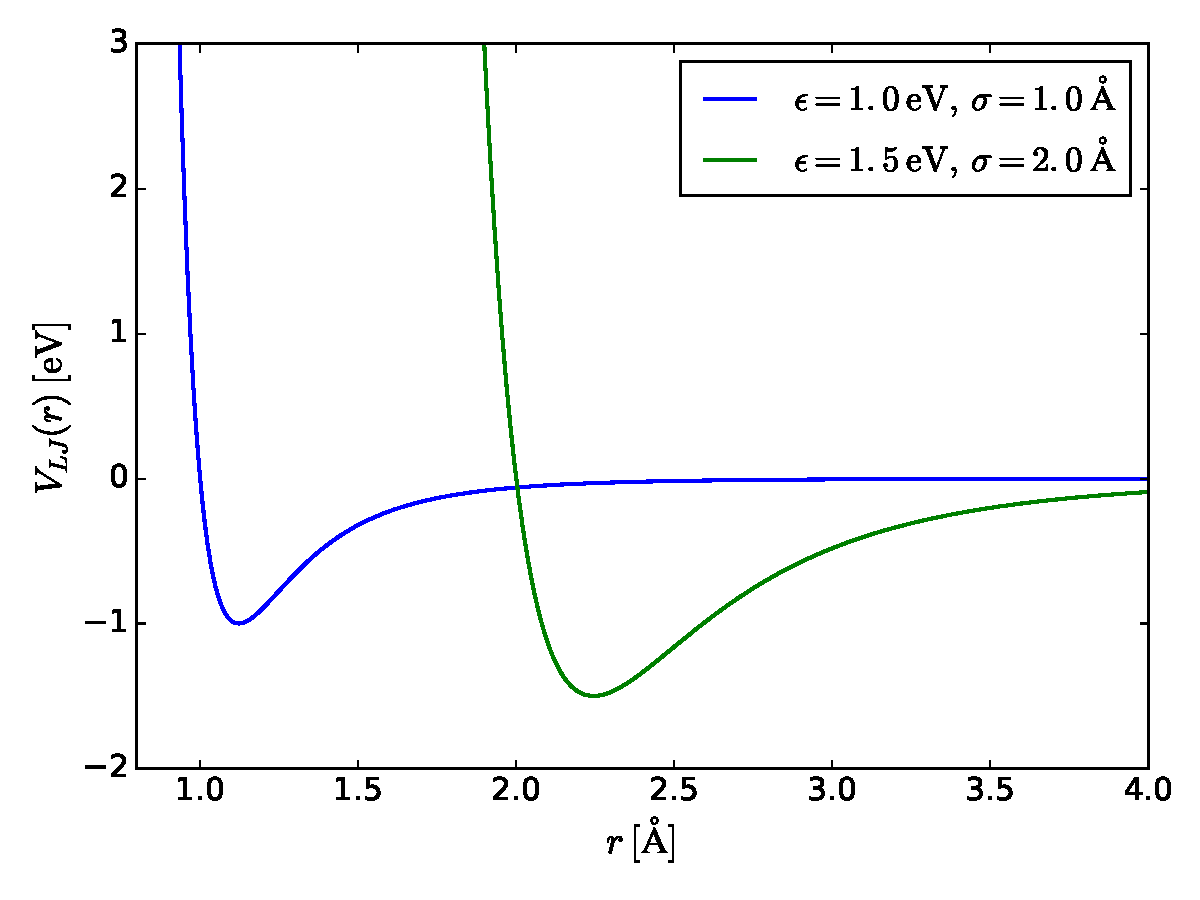
\includegraphics[width = 0.8\linewidth]{Figures/Theory/LJ.pdf}
 \caption{The Lennard-Jones potential \eqref{Lennard-Jones} as a function of inter-atomic distance for two different parameter sets. 
 The depth of the potential well (potential
 strength) is given by $\epsilon$, while $\sigma$ is the inter-atomic distance for which the potential is zero.}
 \label{fig:LJ}
\end{center}
\end{figure}




\subsubsection{Calculating total potential energy}
Before we move on to three-body potentials, we will briefly explain how the total potential energy of a system is calculated. 
For a two-body potential like LJ, each unique pair of atoms is only counted once, so that
\begin{equation}
 V_{\mathrm{tot}} = \sum_{i<j} V_2(r_{ij}) = \frac{1}{2}\sum_{i\neq j} V_2(r_{ij})
 \label{twoBodyPotentialEnergy}
\end{equation}
In the second expression we count all pairs twice, thus a factor $1/2$ is required. 
For the three-body case, the counting is a bit more complicated. An atomic triplet is defined by the three
variables $(r_{ij}, r_{ik}, \theta_{jik}$), where $r_{ij}$ and $r_{ik}$ are the 
two inter-atomic distances to the central atom $i$, and $\theta_{jik}$ is the angle between the lines from $i$ to $j$ and 
from $i$ to $k$. Note that there are only two \textit{independent} variables, since
\begin{equation}
 \theta_{jik} = \frac{\vec{r}_{ij} \cdot \vec{r}_{ik}}{r_{ij}^2r_{ik}^2}
\end{equation}
\autoref{fig:triplets} illustrates that three atoms $(i, j, k)$ define three different triplets depending
on which atom that is the central one. All three triplets have different energies, and must therefore be tallied individually.
If we assume that the potential form is such that it is symmetric with respect to exchange of the $j$ and $k$
indicies (which is not always the case for multielemental systems), we have
\begin{equation}
 \sum_{i<j<k}\left[V_3^{(1)}(r_{ij}, r_{ik}, \theta_{jik}) + V_3^{(2)}(r_{ij}, r_{jk}, \theta_{ijk}) + 
 V_3^{(3)}(r_{ik}, r_{jk}, \theta_{ikj})\right]
 \label{threeBodyPotentialEnergy1}
\end{equation}
\begin{figure}
\begin{center}
 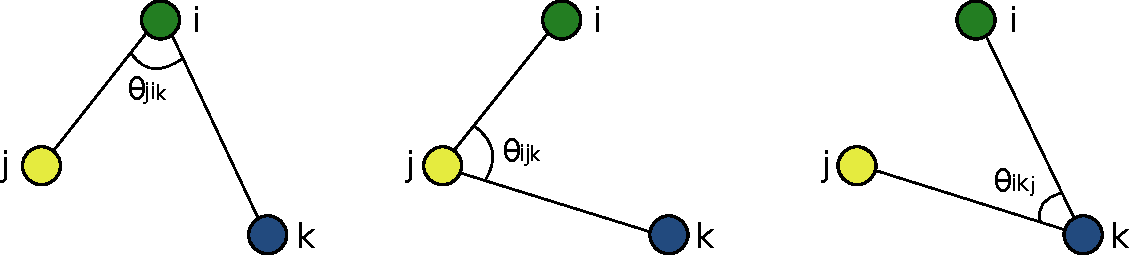
\includegraphics[width = 0.9\linewidth]{Figures/Theory/triplets.pdf}
 \caption{}
 \label{fig:triplets}
\end{center}
\end{figure}
where $V_3^{(i)}$ is one of the triplets in \autoref{fig:triplets}. Alternatively, we can calculate the energy of one triplet 
at a time and instead sum over all $j$,
\begin{equation}
 \sum_{i}\sum_{j\neq i}\sum_{k>j} V_3 (r_{ij}, r_{ik}, \theta_{jik}) 
 \label{threeBodyPotentialEnergy2}
\end{equation}
This is the strategy we are going to adopt in the following. 
The total energy is now written,
\begin{equation}
 V_{\mathrm{tot}} = \sum_i\sum_{j>i} V_2(r_{ij}) + \sum_{i}\sum_{j\neq i}\sum_{k>j} V_3 (r_{ij}, r_{ik}, \theta_{jik}) 
 \label{totalPotentialEnergy}
\end{equation}


\subsection{Stillinger-Weber}
The Stillinger-Weber (SW) potential was proposed in 1985 \cite{Stillinger85} for simulating Si atoms. It has a two-body
and a three-body term, and is thus written on the form \eqref{totalPotentialEnergy}. 
The two-body part consists of a Lennard-Jones factor with variable exponents, together with an exponential decay factor
that ensures zeroing out of the potential at a \textit{cutoff} $a\sigma$,
\begin{equation}
 V_2(r_{ij}) = A\epsilon\left[B\left(\frac{\sigma}{r_{ij}}\right)^p - 
 \left(\frac{\sigma}{r_{ij}}\right)^q\right] \exp\left(\frac{\sigma}{r_{ij} - a\sigma}\right)
\end{equation}
Silicon forms 4-coordinated
tetrahedral bonded structures, and the purpose of the three-body component is to enforce the tetrahedral bond angle
$\theta_0 \approx 109^\circ$, 
\begin{equation}
 V_3(r_{ij}, r_{ik}, \theta_{jik}) = \lambda\epsilon[\cos\theta_{jik} - \cos\theta_0]^2
 \exp\left(\frac{\gamma\sigma}{r_{ij} - a\sigma}\right)\exp\left(\frac{\gamma\sigma}{r_{ik} - a\sigma}\right)
\end{equation}
We observe that for $\theta_{jik} = \theta_0$, the three-body term is zeroed out, making this configuration energetically 
favourable. The expression also contains two exponential decay factors to ensure that the potential goes 
to zero once $r_{ij}$ and/or $r_{ik}$ approach the cutoff. 

SW simulations of solid and liquid silicon agree reasonably well with experimental data \cite{Stillinger85}
The potential has also been used on other systems than silicon, for instance in monatomic water models \cite{Molinero08}. 

\subsection{Vashishta}
In 1990, Vashishta et al. \cite{Vashishta90} suggested a three-body interaction potential for $\mathrm{SiO}_2$. 
The three-body term is of similar form to that of Stillinger-Weber, 
\begin{equation}
\begin{aligned}
 V_3(r_{ij}, r_{ik}, \theta_{jik}) \: = \:
 &B_{jik}\frac{[\cos\theta_{jik} - \cos\theta_{0jik}]^2}{1 + C[\cos\theta_{jik} - \cos\theta_{0jik}]^2} \: \cdot \\
 &\exp\left(\frac{\gamma_{ij}}{r_{ij} - r_{0ij}}\right)
 \exp\left(\frac{\gamma_{ik}}{r_{ik} - r_{0ik}}\right)
\end{aligned}
\end{equation}
We note that indicies are included for the parameters, as they are generally different for each pair and triplet combination
of elements; the parameter set must be fitted to e.g. Si-Si-Si and Si-O-O seperately. The angle $\theta_{0jik}$ has 
the same purpose as for SW, while $r_{0ij}$ is the cutoff distance for each pair of elements. 

\noindent The two-body part is more complex,
\begin{equation}
 V_2(r_{ij}) = \frac{H_{ij}}{r^{\eta_{ij}}} - \frac{W_{ij}}{r^6} + \frac{Z_iZ_j}{r}\exp(-r/\lambda_{1,ij}) - 
 \frac{D_{ij}}{r^4}\exp(-r/\lambda_{4,ij}) 
\end{equation}
where we recognize the two first terms as typical LJ repulsive and attractive components. The other two describe
electrostatic interactions, the third being a so-called screened Coulomb potential for charges $Z_i$ and $Z_j$. 
We will not expand upon the physical justification of these terms here. 

The Vashishta potential has also been succesfully employed on other multi-component systems like SiC \cite{Vashishta07}. 


\section{Time integration}
To evolve the system forward in time, we need a numerical method to integrate Newton's equations of motion,
\begin{align}
 \vec{v}(t) = \vec{v}(0) + \int_0^t\vec{a}(t)dt \label{equationsOfMotion1} \\
 \vec{r}(t) = \vec{r}(0) + \int_0^t\vec{v}(t)dt
 \label{equationsOfMotion2}
\end{align}
Various finite different schemes can be used for this purpose, and the choice of algorithm is 
of vital importance to the quality of the simulation. The most important property of an integrator
for use in MD, is long-term energy conservation. MD simulations are often run for millions of time steps, 
and a significant energy drift may cause useless results. Further, all integration schemes approximate 
derivatives as finite differences, introducing truncation errors. Finally, numerical stability is
important to prevent unphysical behaviour on large time scales. 

A good choice is the Velocity-Verlet algorithm, which is
a \textit{symplectic} integrator. Put simply, this means that it preserves the form of Hamilton's equations, thereby
conserving energy. \footnote{Strictly speaking, Velocity-Verlet only conserves a pseudo-Hamiltonian
approaching the true Hamiltonian in the limit of infinitesimal time steps. \cite{Frenkel01}}
Employing Velocity-Verlet
allows us to sample the phase space of the microcanonical (NVE) ensemble, and collect 
thermodynamic properties like temperature and pressure.
The steps of the algorithm are,
\begin{align}
 \vec{v}(t + \Delta t/2) &= \vec{v}(t) + \frac{\vec{F}(t)}{m}\frac{\Delta t}{2} \\
 \vec{r}(t + \Delta t) &= \vec{r}(t) + \vec{v}(t + \Delta t/2)\Delta t \\
 \vec{v}(t + \Delta t) &= \vec{v}(t + \Delta t) + \frac{\vec{F}(t + \Delta t)}{m}\frac{\Delta t}{2}
\end{align}
First, the velocity at half the time step forward $\vec{v}(t + \Delta t/2)$ is computed. 
This half-velocity is used to obtain the new positions $\vec{r}(t + \Delta t)$. 
Then we calculate the new accelerations $\vec{F}(t+\Delta t)/m$ based on the new positions, which is used
to compute the velocities at a whole time step forward $\vec{v}(t + \Delta t)$. 

In addition to being symplectic, Velocity-Verlet is time-reversible \cite{Frenkel01}, which it should be considering that we 
are solving time-reversible equations \eqref{equationsOfMotion1} \eqref{equationsOfMotion2}. 
It is also computationally inexpensive; the only 
additional computation compared to the primitive Euler method is the half-velocity. 
The global error in position and velocity is $O(\Delta t^2)$, which may not seem very impressive. However, 
this is good enough for collecting statistical properties, 
our goal is not to reproduce the exact trajectories of the particles. 

Velocity-Verlet is the integrator of choice in LAMMPS (\autoref{sec:lammps}), and thus the 
only scheme used in this work. 

\section{Force calculations and cutoff radius} \label{sec:forceCutoff}
We need the force on each atom to compute the acceleration that is integrated in the equations of motion
\eqref{equationsOfMotion1}\eqref{equationsOfMotion2}. 
Using the Lennard-Jones potential as an example, 
the force on atom $i$ from atom $j$ is \eqref{forcePES} \eqref{Lennard-Jones},
\begin{equation}
 F_{\mathrm{LJ}}(r_{ij}) = -\nabla V_{\mathrm{LJ}}(r_{ij}) = 
 -24\epsilon\left[2\left(\frac{\sigma^{12}}{r_{ij}^{13}}\right) - \left(\frac{\sigma^6}{r_{ij}^7}\right)\right] 
\end{equation}
The force is of the same shape 
as the potential in \autoref{fig:LJ}, which means it rapidly goes to zero. If we choose units so that
$\sigma=\epsilon=1.0$, the force at a distance $r_{ij} = 3\sigma$ is
\begin{equation}
 F_{\mathrm{LJ}}(r_{ij} = 3.0\sigma) \approx 0.01
\end{equation}
This is a general property of systems where only van der Waal-interactions are present: atoms that 
are far apart do not effectively interact. This can be exploited in MD simulations by introducing 
a cutoff radius $r_{\mathrm{cut}}$, and only compute forces for atoms displaced by a distance smaller than this cutoff. 
In principle, we have to sum over all pairs of atoms in the system to compute the energy and forces, which 
scales like $O(N^2)$. With a cutoff, this is reduced to $O(N)$, and the force is now written,
\begin{equation}
 F_{\mathrm{LJ}}(r_{ij}) = 
 \begin{cases}
  -24\epsilon\left[2\left(\frac{\sigma^{12}}{r_{ij}^{13}}\right) - \left(\frac{\sigma^6}{r_{ij}^7}\right)\right] ,
  & r_{ij} \leq r_{\mathrm{cut}} \\
  0, & r_{ij} > r_{\mathrm{cut}} 
 \end{cases}
 \label{forceCutoff}
\end{equation}
and similar for the potential energy \eqref{Lennard-Jones}. 
This greatly increases the computational performance of MD simulations. In fact, simulations with non-bonded potentials
not including a cutoff is unfeasible except for small systems. 



\chapter{Machine learning} \label{sec:machineLearning}
Machine learning is the science of giving computers the ability to learn without being explicitly programmed. 
The idea is that there exist generic algorithms which can be used to find patterns in a broad class of data sets without 
having to write code specifically for each problem. The algorithm will build its own logic based on the data.  

Machine learning is a subfield of computer science, and is closely related to computational statistics. 
It evolved from the study of pattern recognition in artificial intelligence research (AI), and has made contributions to
AI tasks like computer vision, natural language processing and speech recognition. It has also, especially in later years, 
found applications in a wide variety of other areas, including bioinformatics, economy, physics, finance and marketing. 
(SHOULD I HAVE REFERENCES HERE??)

The approaches to machine learning are many, but are often split into two main categories. 
In \textit{supervised learning} we know the answer to a problem,
and let the computer deduce the logic behind it. On the other hand, \textit{unsupervised learning}
is a method for finding patterns and relationship in data sets withouth any prior knowledge of the system.
Some authours also operate with a third category, namely \textit{reinforcement learning}. This is a paradigm 
of learning inspired by behavioural psychology, where learning is achieved by trial-and-error, 
solely from rewards and punishment.

Another way to categorize machine learning tasks is to consider the desired output of a system.
Some of the most common tasks are:
\begin{itemize}
 \item Classification: Outputs are divided into two or more classes. The goal is to 
 produce a model that assigns inputs into one of these classes. An example is to identify
 digits based on pictures of hand-written ones. Classification is typically supervised learning.  
 \item Regression: Finding a functional relationship between an input data set and a reference data set. 
 The goal is to construct a function that maps input data to continous output values. 
 \item Clustering: Data are divided into groups with certain common traits, without knowing the different groups beforehand.
 It is thus a form of unsupervised learning.  
\end{itemize} 
\autoref{fig:machineLearningDiagram} gives an (incomplete) overview of machine learning methods with some selected applications.
We will not go into further detail on all these approaches to machine learning, as this work only concerns
one specific area of ML: artificial neural networks. The rest of this chapter concerns the ideas behind this machine learning
approach. 
\begin{figure}
\begin{center}
 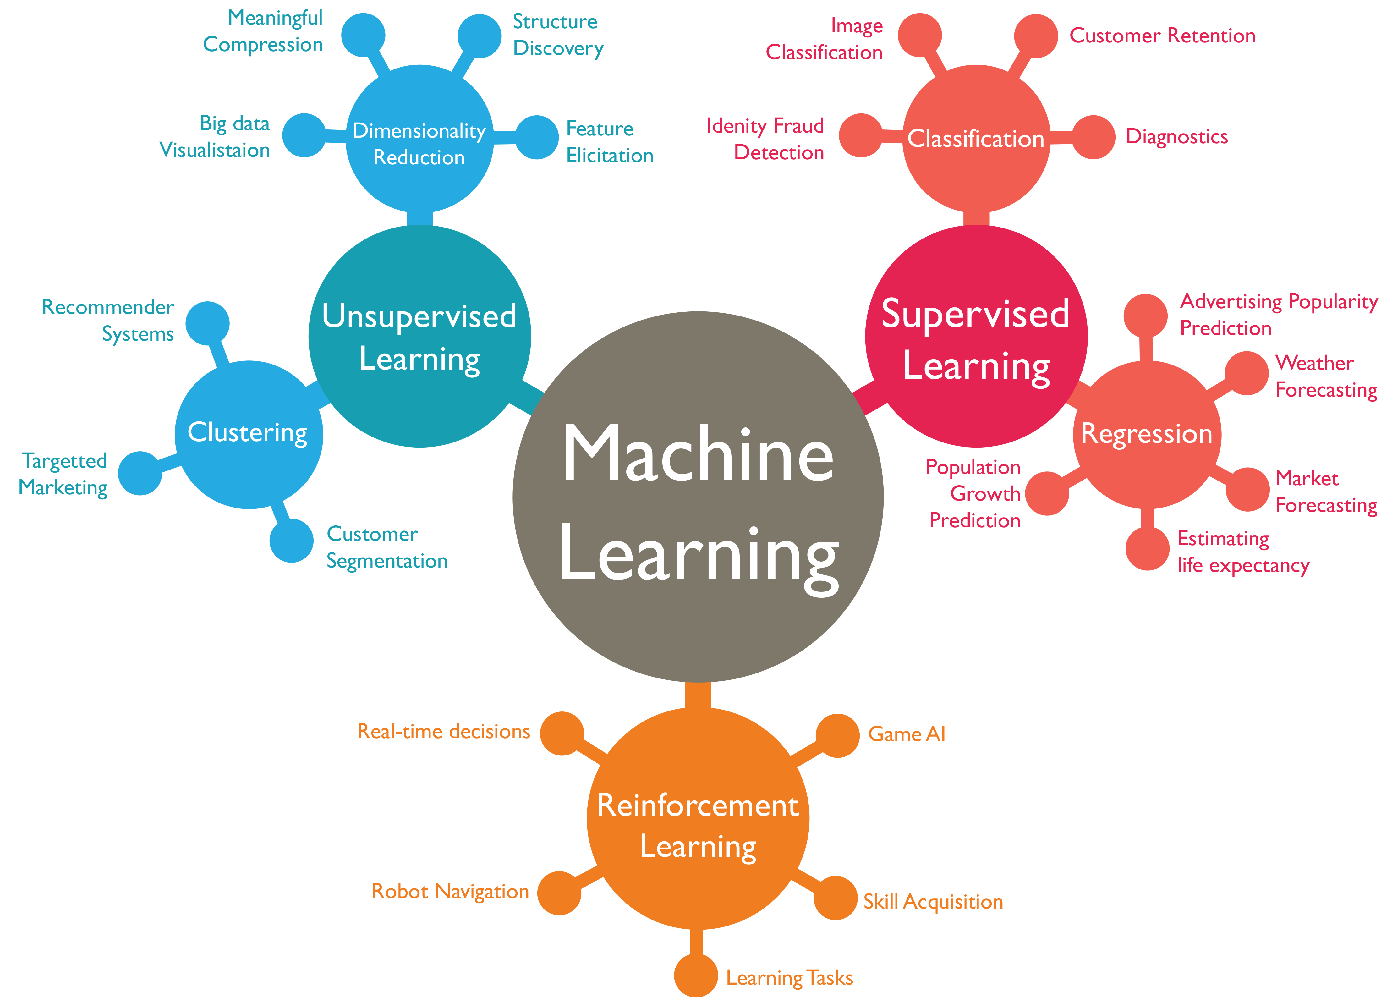
\includegraphics[width = \linewidth]{Figures/Theory/MachineLearningDiagram.png}
 \caption{Machine learning, taken from from http://www.isaziconsulting.co.za/machinelearning.html.}
 \label{fig:machineLearningDiagram}
\end{center}
\end{figure}

\section{Artificial neurons} \label{sec:ANN}
The field of artificial neural networks has a long history of development, and is closely connected with 
the advancement of computer science and computers in general. A model of artificial neurons 
was first developed by McCulloch and Pitts in 1943 \cite{McCulloch43} to study signal processing in the brain and 
has later been refined by others. The general idea is to the mimic neural networks in the human brain, which
is composed of billions of neurons that communicate with each other by sending electrical signals. 
Each neuron accumulates its incoming signals, 
which must exceed an activation threshold to yield an output of one. If the threshold is not overcome, the neuron
remains inactive, i.e. has zero output.  

This behaviour has inspired a simple mathematical model for an artificial neuron \cite{Rojas96},
\begin{equation}
 y = f\left(\sum_{i=1}^n w_ix_i\right) = f(u)
 \label{artificialNeuron}
\end{equation}
Here, the output $y$ of the neuron is the value of its activation function, which have as input
a weighted sum of signals $x_i, \dots ,x_n$ received by $n$ other neurons.
The model is illustrated in \autoref{fig:neuronModel}. We will now take a closer look at if and how 
this mathematical model is biologically plausible.
\begin{figure}
 \begin{center}
  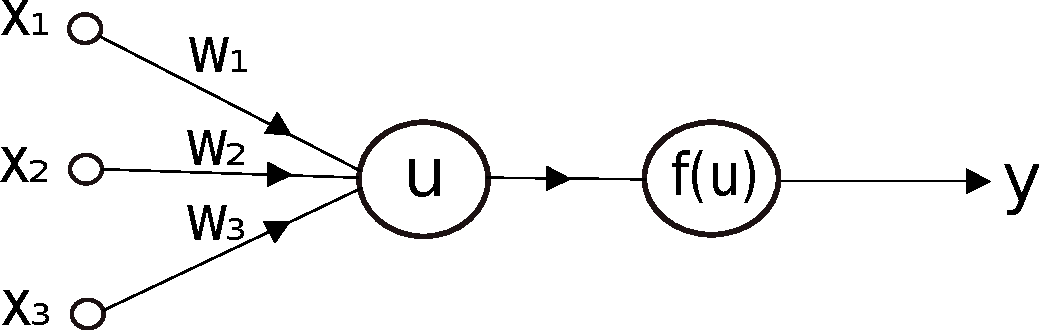
\includegraphics[width=\linewidth]{Figures/Theory/neuron.pdf}
  \caption{Mathematical model of an artificial neuron. The neuron receives input signals $x_i,\dots,x_n$ from
	   $n$ other neurons. Each signal $x_i$ is associated with a weight $w_i$, and the neuron accumulates
	   all input signals as a weighted sum $u$. This sum is then used as input to its activation function
	   $f$, which serves as the neuron's output signal.}
  \label{fig:neuronModel}
 \end{center}
\end{figure}

\subsection*{Biological model}
Artificial neurons are designed to mimic certain aspects of their biological counterparts \cite{Kriesel07}. 
A schematic model of a biological nervous cell is depicted in \autoref{fig:neuronBiological}.
The \textit{dendrites} in a neuron acts as the input vector, and allow the cell to receive signals from a large number
of neighbouring neurons. As in the mathematical model, each dendrite is associated with the multiplication of a
''weight value'', which is achieved by an increase or decrease of chemical neurotransmitters that amplifies or
weakens the input signals. The cell can also transmit signal inhibitors (oppositely charged ions) to 
accomplish ''negative'' weight values. 

The positive and negative ions arriving from the dendrites are mixed together in the solution inside the \textit{soma}. 
which corresponds to the summation in \eqref{artificialNeuron}. Finally, the \textit{axon} serves
as the activation function by sampling the electrical potential of this solution. If the potential 
reaches a certain strength, the axon transmits a signal pulse down its own length. The axon is connected 
to another neuron's dendrites (or other parts of the cell), enabling the neurons to communicate. 
\begin{figure}
 \begin{center}
  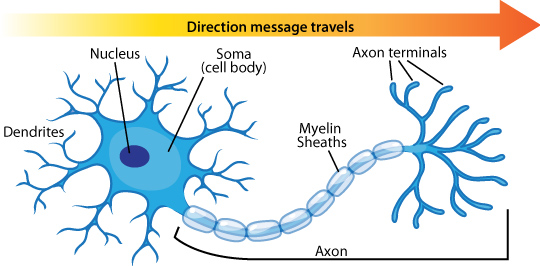
\includegraphics[width=\linewidth]{Figures/Theory/neuron_anatomy.jpg}
  \caption{Biological model of a neuron. 
	   Source: \href{https://askabiologist.asu.edu/neuron-anatomy}{https://askabiologist.asu.edu/neuron-anatomy}}
  \label{fig:neuronBiological}
 \end{center}
\end{figure}

This discussion of nervous cells helps, to a certain degree, to validate the mathematical form \eqref{artificialNeuron}
of artifical neurons. However, we note that the above description is a highly simplified picture of the great complexity
of biological neurons, which is not yet fully understood. Our mathematical neurons are thus only caricatures of nature. 
Next, we will look at how networks of these mathematical objects can be formed to emulate the neural networks
in the brain.

\section{Neural network types}
An artificial neural network (ANN), is a computational model that consists of layers of connected neurons, or \textit{nodes}. 
It is supposed to mimic a biological nervous system by letting each neuron interact with other neurons
by sending signals in the form of mathematical functions between layers. 
Each node is modelled according to \eqref{artificialNeuron}. 
A wide variety of different ANNs have
been developed, but most of them consist of an input layer, an output layer and eventual layers in-between, called
\textit{hidden layers}. All layers can contain an arbitrary number of nodes, and each connection between two nodes
is associated with a weight variable. 

The main factor that seperates the different types are how the neurons are \textit{connected}. 
This section contains a short presentation of some of the most common types of ANNs, before we move on to 
a more detailed description of the ANN architecture used in this thesis. In the following we will refer to artificial 
neural networks simply as neural networks (NNs), i.e. not referring to its biological counterpart.  

\subsection{Feed-forward neural networks}
The feed-forward neural network (FFNN) was the first and simplest type of NN devised. In this network, 
the information moves in only one direction - forward through the layers. An example FFNN is shown
in \autoref{fig:networkGeneral}, which consists of an input layer, two hidden layers and an output layer. 
Nodes are represented by circles, while the arrows display the connections between the nodes, including the 
direction of information flow. Additionaly, each arrow corresponds to a weight variable, not displayed here. 
We observe that each node in a layer is connected to \textit{all} nodes in the subsequent layer, 
making this a so-called \textit{fully-connected} FFNN. 
This is the type of NN that is used in the present work, 
and will be further investigated in chapter (REF TO CHAPTER).
\begin{figure}
 \begin{center}
  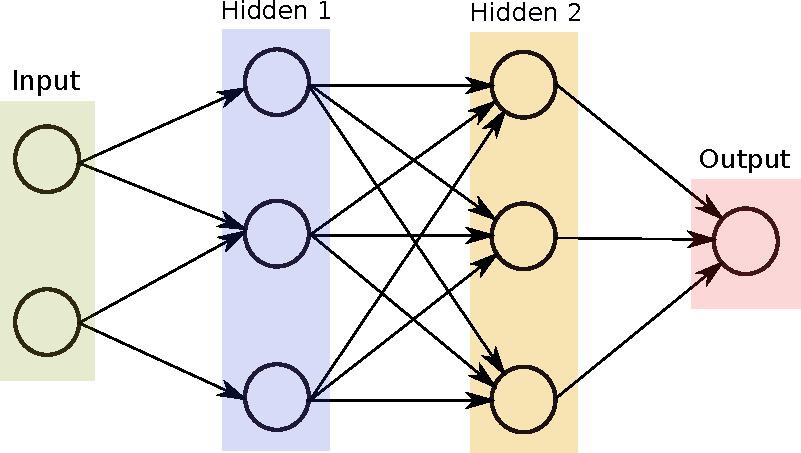
\includegraphics[width=\linewidth]{Figures/Theory/networkGeneral.pdf}
  \caption{Example of a fully-connected feed-forward neural network with an input layer, two hidden layers
	   and an output layer. Each node in a layer is connected to \textit{all} nodes in the subsequent layer, 
	   and information only flows forward through the layers, hence the name.}
  \label{fig:networkGeneral}
 \end{center}
\end{figure}

A different variant of FFNNs are \textit{convolutional neural networks} (CNNs) \cite{LeCun99}, which have a connectivity pattern
inspired by the animal visual cortex. Individual neurons in the visual cortex only respond to stimuli from
small sub-regions of the visual field, called a receptive field. This makes the neurons well-suited to exploit the strong
spatially local correlation present in natural images. The response of each neuron can be approximated mathematically 
as a convolution operation. 

CNNs emulate the behaviour of neurons in the visual cortex by enforcing a \textit{local} connectivity pattern
between nodes of adjacent layers: Each node
in a convolutional layer is connected to a subset of the nodes in the previous layer, 
in contrast to the fully-connected FFNN in \autoref{fig:networkGeneral}.
Often, CNNs 
consist of several convolutional layers that learn local features of the input, with a fully-connected layer at the end, 
which gathers all the local data and produces the outputs. They have wide applications in image and video recognition. 

\subsection{Recurrent neural networks}
So far we have only mentioned NNs where information flows in one direction: forward. \textit{Recurrent neural networks} on
the other hand, have connections between nodes that form directed \textit{cycles}. This creates a form of 
internal memory which are able to capture information on what has been calculated before; the output is dependent 
on the previous computations. Recurrent NNs make use of sequential information by performing the same task for 
every element in a sequence, where each element depends on previous elements. An example of such information is 
sentences, making recurrent NNs especially well-suited for handwriting and speech recognition.

\subsection{Other types of networks}
There are many other kinds of NNs that have been developed. One type that is specifically designed for interpolation
in multidimensional space is the radial basis function (RBF) network. RBFs are typically made up of three layers: 
an input layer, a hidden layer with non-linear radial symmetric activation functions and a linear output layer (''linear'' here
means that each node in the output layer has a linear activation function). The layers are normally fully-connected and 
there are no cycles, thus RBFs can be viewed as a type of fully-connected FFNN. They are however usually treated as
a seperate type of NN due the unusual activation functions (common activation functions are presented in chapter
(REF TO CHAPTER)) 
and a different training algorithm, that we will not expand upon 
here. 

Other types of NNs could also be mentioned, but are outside the scope of this work. Now we will move on to a detailed description
of how a fully-connected FFNN functions, and how it can be trained to interpolate data. 

\section{Multilayer perceptron}
In this thesis we use fully-connected feed-forward neural networks with three
or more layers (an input layer, one or more hidden layers and an output layer), mainly
consisting of neurons that have non-linear activation functions.
Such networks are often called \textit{multilayer perceptrons} (MLPs). 
\footnote{The terms ''feed-forward neural network'' and ''multilayer perceptron'' are used interchangeably in the 
literature, although the MLP is just one type of FFNN, namely a fully-connected one with mainly non-linear neurons.}
The \textit{perceptron} was first introduced by Rosenblatt in 1958 \cite{Rosenblatt58}, and was a FFNN made up of an input layer
and an ouput layer only. It served as a \textit{binary classifier}, i.e. a function that maps a real-valued vector $\vec{x}$ 
to a single binary value $f(\vec{x})$, employing a linear activation function. The addition of hidden layers and 
non-linear activation functions led to the MLP, which could produce an arbitrary number of continous output values. 

\subsection{Why multilayer perceptrons?} \label{sec:whyMLP}
We have chosen to use MLPs to interpolate data sets for the construction of inter-atomic potentials. 
Other NN types could also have been used, but our choice is well justified. According to the
\textit{Universal approximation theorem} \cite{Hornik89}, a feed-forward neural network with just a single hidden layer containing 
a finite number of neurons can approximate a continous multidimensional function to arbitrary accuracy, 
assuming the activation function for the hidden layer is a ''non-constant, bounded and monotonically-increasing continous function''.
Note that the requirements on the activation function only applies to the hidden layer, the output nodes are always
assumed to be linear, so as to not restrict the range of output values. 
The only requirement on the NN information flow is that it must be feed-forward, thus recurrent NNs are out of the picture. 
Also, we might as well use the simplest multilayer FFNN available, the MLP, as 
adding complicating factors like local connectivity is unnecessary for our purposes. 

We note that this theorem is only applicable to a NN with \textit{one} hidden layer. Therefore, we can easily construct a NN 
which employs activation functions that do not satisfy the above requirements, as long as we have at least one layer
with activation functions that \textit{do}. Furthermore, although the universal approximation theorem
lays the theoretical foundation for regression with neural networks, it does not say anything about how things work in practice: 
a NN can still be able to approximate a given function reasonably well without having the flexibility to fit \textit{all other}
functions. 

\subsection{Mathematical model} \label{sec:MLPmodel}
In an MLP, each node (neuron) is modelled according to \eqref{artificialNeuron}. To increase the flexibility of the NN,
we also add a \textit{bias} to this model, resulting in 
\begin{equation}
 y = f\left(\sum_{i=1}^n w_ix_i + b_i\right) = f(u)
 \label{artificialNeuron2}
\end{equation}
In a FFNN of such neurons, the \textit{inputs} $x_i$
are the \textit{outputs} of the neurons in the preceding layer. Furthermore, a MLP is fully-connected, 
which means that each neuron receives a weighted sum of the outputs of \textit{all} neurons in the previous layer. 

\autoref{fig:networkNotation} displays the same NN as in \autoref{fig:networkGeneral}, now with all nodes labeled by their
output $y$, except for the input nodes, which are labeled with $x$. The input nodes are strictly speaking not 
artifical neurons, as they have no activation function. Their only purpose is to forward the NN inputs to the 
first hidden layer. A few weights $w$ (blue) and biases $b$ (green) are also included, next to the connections and nodes
which they belong to respectively. 
\begin{figure}
 \begin{center}
  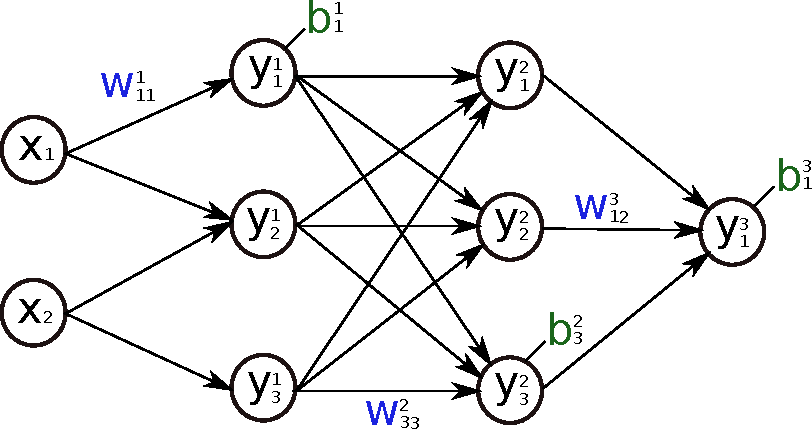
\includegraphics[width=\linewidth]{Figures/Theory/networkWithNotation.pdf}
  \caption{Example of a fully-connected feed-forward neural network with an input layer, two hidden layers
	   and an output layer. Nodes are depicted as circles, while the arrows shows the connections between neurons, 
	   including their directions. Each connection has a weight $w$ (blue), where the notation explained in the
	   text is applied. Every node is marked with its output $y$ and its associated bias $b$ (green), while all input nodes
	   are labeled with an $x$. Only a few weights and biases are listed.}
  \label{fig:networkNotation}
 \end{center}
\end{figure}
The following notation is introduced: $y_i^l$ is the output of the $i$-th node in layer $l$, where $l=0$ is the input layer, 
$l=1$ is the first hidden layer and so on. The same notation applies to the biases. For the weights, we have that
$w_{ij}^l$ is the weight connecting node $j$ in layer $l-1$ with node $i$ in layer $l$. 
\footnote{This order of indicies $i$ and $j$ may seem illogical, but will become useful when converting
the equations below to matrix equations.}
All weights and biases are real-valued numbers.

The MLP in \autoref{fig:networkNotation} maps the inputs $x_i$ to the output $y_1^3$ via two hidden layers
with an (arbitrary) number of hidden nodes. The hidden neurons have no physical meaning, but have the purpose
of defining the functional form of the NN. In the following we describe how to calculate the output of this MLP. The description
is also valid for a NN with several outputs; the result applies to each ouput node individually. 

First, for each node $i$ in the first hidden layer, we calculate a weighted sum $u_i^1$ of the input coordinates $x_m$,
\begin{equation}
 u_i^1 = \sum_{j=1}^2 w_{ij}^1 x_j  + b_i^1 
\end{equation}
This value is the argument to the activation function $f^1$ of each neuron,
producing the output $y_i^1$ of all neurons in layer 1,
\begin{equation}
 y_i^1 = f^1(u_i^1) = f^1\left(\sum_{j=1}^2 w_{ij}^1 x_j  + b_i^1\right)
 \label{outputLayer1}
\end{equation}
where we assume that all nodes in the same layer have identical activation functions, hence the notation $f^l$. 
For an arbitrary node $i$ in layer $l$ this generalizes to
\begin{equation}
 y_i^l = f^l(u_i^l) = f^l\left(\sum_{j=1}^{N_{l-1}} w_{ij}^l y_j^{l-1} + b_i^l\right)
 \label{generalLayer}
\end{equation}
where $N_l$ is the number of nodes in layer $l$. When the output of all the nodes in the first hidden layer are computed,
the values of the subsequent layer can be calculated and so forth until the output is obtained. 
The output of neuron $i$ in layer 2 is thus,
\begin{align}
 y_i^2 &= f^2\left(\sum_{j=1}^3 w_{ij}^2 y_j^1 + b_i^2\right) \\
 &= f^2\left[\sum_{j=1}^3 w_{ij}^2f^1\left(\sum_{k=1}^2 w_{jk}^1 x_k + b_j^1\right) + b_i^2\right]
 \label{outputLayer2}
\end{align}
where we have substituted $y_m^1$ with \eqref{outputLayer1}. Finally, the NN output yields,
\begin{align}
 y_1^3 &= f^3\left(\sum_{j=1}^3 w_{1m}^3 y_j^2 + b_1^3\right) \\
 &= f^3\left[\sum_{j=1}^3 w_{1j}^3 f^2\left(\sum_{k=1}^3 w_{jk}^2 f^1\left(\sum_{m=1}^2 w_{km}^1 x_m + b_k^1\right) + b_j^2\right)
  + b_1^3\right]
\end{align}
We can generalize this expression to a MLP with $l$ hidden layers. The complete functional form
is,
\begin{equation}
 y^{l+1}_1 = f^{l+1}\left[\sum_{j=1}^{N_l} w_{1j}^3 f^l\left(\sum_{k=1}^{N_{l-1}} w_{jk}^2 f^{l-1}\left(
 \cdots f^1\left(\sum_{n=1}^{N_0} w_{mn}^1 x_n + b_m^1\right)
 \cdots \right) + b_k^2\right)
 + b_1^3\right]
 \label{completeNN}
\end{equation}
which illustrates a basic property of MLPs: the only independent variables are the input values $x_j$. 
This confirms that a MLP,
despite its quite convoluted mathematical form, is nothing more than an analytic function, specifically a 
mapping of real-valued vectors $\vec{x} \in \mathbb{R}^n \rightarrow \vec{y} \in \mathbb{R}^m$. 
In our example (\autoref{fig:networkNotation}), $n=2$ and $m=1$. Consequentially, 
the number of input and output values of the function we want to fit must be equal to the number of inputs and outputs of our MLP.  

Furthermore, the flexibility and universality of a MLP can be illustrated by realizing that 
the expression \eqref{completeNN} is essentially a nested sum of scaled activation functions of the form
\begin{equation}
 h(x) = c_1 f(c_2 x + c_3) + c_4
\end{equation}
where the parameters $c_i$ are weights and biases. By adjusting these parameters, the activation functions
can be shifted up and down or left and right, change slope or be rescaled (\autoref{fig:activationsFlex}), 
which is the key to the flexibility of a NN. 
\begin{figure}
\begin{center}
  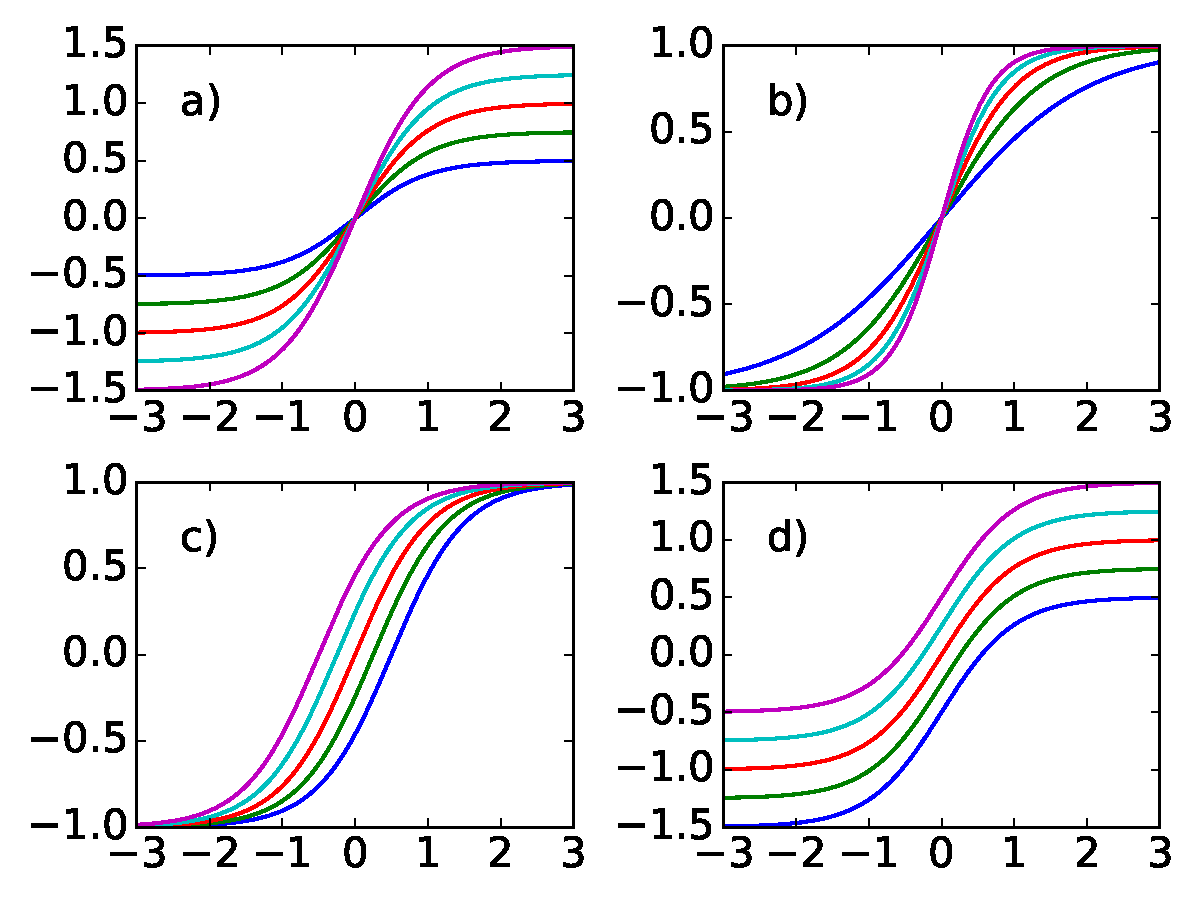
\includegraphics[width = 0.9\linewidth]{Figures/Theory/activationFlex.pdf}
  \caption{The mathematical expression for a MLP consists of nested terms of the form $h(x) = c_1 f(c_2 x + c_3) + c_4$, 
	   where $f$ is the activation function
	    and $c_i$ are NN parameters. The flexibility of the MLP is shown by adjusting $c_1$, $c_2$, $c_3$ and $c_4$ such that
	    $h(x)$
	    a) is scaled, b) has a change of slope, c) is shifted left and right, d) is shifted up and down, respectively.}
  \label{fig:activationsFlex}
  \end{center}
\end{figure}

\subsubsection{Activation function of output neuron}
We stated in \autoref{sec:whyMLP} that the output neuron always have a linear activation function for regression to avoid
restricting the output values. This is a requirement for a MLP to operate as a mapping 
$\vec{x} \in \mathbb{R}^n \rightarrow \vec{y} \in \mathbb{R}^m$. In this thesis, we will exclusively use a
specific linear activation function for the output neuron $o$, namely the identity function $f(x) = x$,
\begin{equation}
 f_o = f(u_o) = u_o
 \label{outputActivation}
\end{equation}



\subsubsection{Matrix representation}
We can introduce a more convenient notation for the activations in a NN. 
If we look at the structure of the NN in \autoref{fig:networkNotation}, we realize that all the weights connecting 
two adjacent layers can be represented as a matrix $W$, where $w_{ij} = w^l_{ij}$ is the weight connecting connecting node $j$
in layer $l-1$ with node $i$ in layer $l$. Additionaly, we can represent the biases and activations
as layer-wise column vectors $\vec{b}$ and $\vec{y}$, so that $b_i = b_i^l$ is the bias of node $i$ in layer $l$. 
We have that $W_l$ is a $N_{l-1} \times N_l$ matrix, while $\vec{b}_l$ and $\vec{y}_l$ are $N_l \times 1$ column vectors. 

With this notation, the sum in \eqref{outputLayer2} becomes a matrix-vector multiplication, and we can write
the equation for the activations of hidden layer 2 in \autoref{fig:networkNotation} as
\begin{equation}
 \vec{y}_2 = f(W_2 \vec{y}_{1} + \vec{b}_{2}) = 
 f\left(\left[\begin{array}{ccc}
    w^2_{11} &w^2_{12} &w^2_{13} \\
    w^2_{21} &w^2_{22} &w^2_{23} \\
    w^2_{31} &w^2_{32} &w^2_{33} \\
    \end{array} \right] \cdot
    \left[\begin{array}{c}
           y^1_1 \\
           y^1_2 \\
           y^1_3 \\
          \end{array}\right] + 
    \left[\begin{array}{c}
           b^2_1 \\
           b^2_2 \\
           b^2_3 \\
          \end{array}\right]\right)
\end{equation}
and we see that the activation of node $i$ in layer 2 is
\begin{equation}
 y^2_i = w^2_{i1}y^1_1 + w^2_{i2}y^1_2 + w^2_{i3}y^1_3 + b^2_i = 
 \sum_{j=1}^3 w^2_{ij} y_j^1 + b^2_i
\end{equation} 
which is in accordance with \eqref{outputLayer2}. This is not just a nice and compact notation, but also 
a useful and intuitive way to think about MLPs: the output is calculated by a series of matrix-vector multiplications
and vector additions that are used as input to the activation functions. For each operation 
$W^l \vec{y}^{l-1}$ we move forward one layer. Furthermore, it is the easiest way to implement NNs with 
TensorFlow, which is discussed in \autoref{sec:TensorFlowCreatingNN}. 



\section{Activation functions}
A property that characterizes a NN, other than its connectivity, is the choice of activation function(s). 
As described in \autoref{sec:whyMLP}, the following restrictions are imposed on an activation function for a FFNN
to fulfill the universal approximation theorem \cite{Hornik89}:
\begin{enumerate}
 \item Non-constant
 \item Bounded
 \item Monotonically-increasing
 \item Continous
\end{enumerate}
We realize that the second requirement excludes all linear functions. Furthermore, in a MLP with only linear activation functions, each 
layer simply performs a linear transformation of its inputs. Consequentially, regardless of the number of layers, 
the output of the NN will be nothing but a linear function of the inputs. Thus we need to introduce some kind of 
non-linearity to the NN to be able to fit non-linear functions. 

A group of non-linear functions that meet the above requirements are the \textit{sigmoid} functions. 
The two sigmoid functions that are most commonly used as activation functions \cite{Rojas96} in 
neural networks are the logistic function
\begin{equation}
 f(x) = \frac{1}{1 + e^{-x}}
 \label{sigmoidActivationFunction}
\end{equation}
and the hyperbolic tangent
\begin{equation}
 f(x) = \tanh(x)
 \label{tanhActivationFunction}
\end{equation}
The logistic functon is often referred to as ''the sigmoid'', which is the naming convention we will use 
in the following. Both functions are depicted in \autoref{fig:SigmoidActivationFunctions}. We observe that they
are bounded above by 1, while the lower bound is -1 and 0 for the hyperbolic tangent and sigmoid respectively. This property 
keeps the activations from blowing up. 
\begin{figure}
\begin{center}
  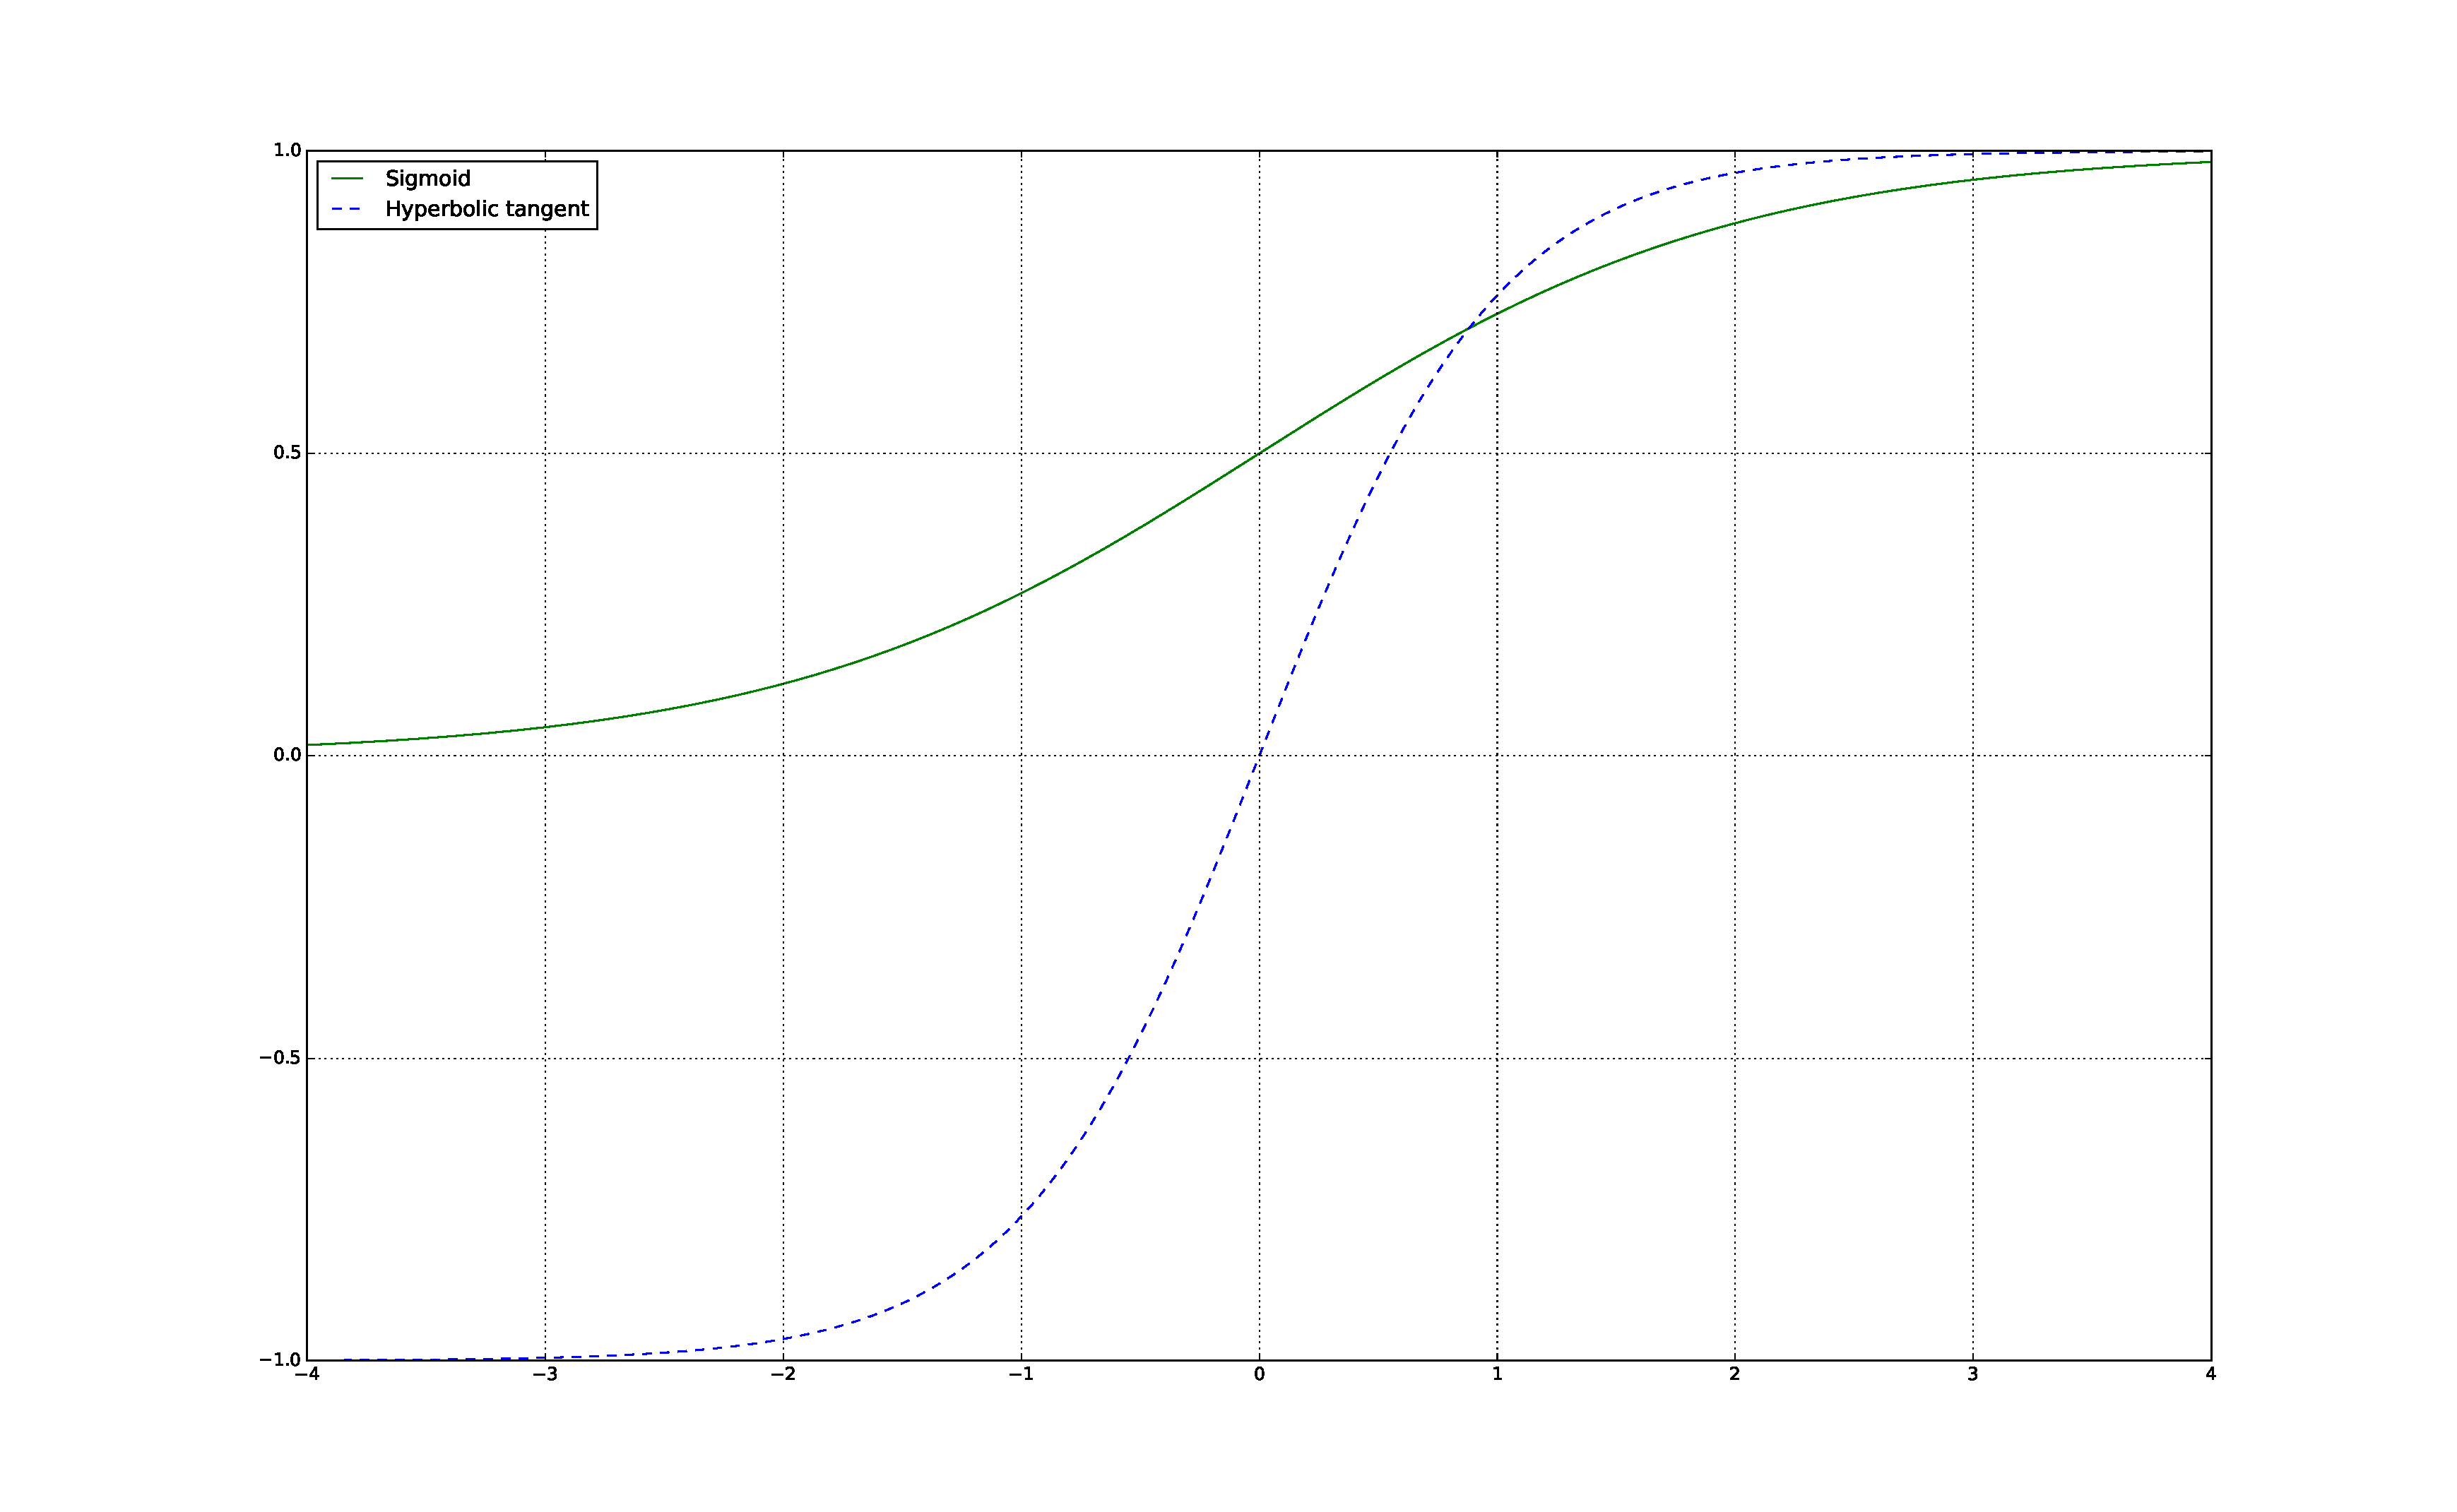
\includegraphics[width = 0.7\linewidth]{Figures/Theory/activationFunctions.pdf}
  \caption{Two of the most common activation functions for neural networks. Both meet the requirements
	   of the universal approximation theorem.}
  \label{fig:SigmoidActivationFunctions}
  \end{center}
\end{figure}
The sigmoid are more bilogically plausible because 
the output of inactive neurons are zero. Such activation function are called \textit{one-sided}. However,
it has been shown \cite{Karlik11} that the hyperbolic tangent 
performs better than the sigmoid for training MLPs. This will be further discussed in section (REF TO SECTION). 
Nevertheless, one should assess the problem 
at hand when deciding what activation function to use; the performance can vary from problem to problem. 

In later years, the rectifier function (\autoref{fig:reluActivationFunction})
\begin{equation}
 f(x) = \max(0,x)
\end{equation}
has become the most popular \cite{LeCun15} for \textit{deep neural networks}, i.e. NNs with a large number of hidden layers.
It has been argued to be even more biologically plausible than the sigmoid and also perform better
than the hyperbolic tangent, especially for deep, convolutional NNs \cite{Glorot11}. Even though the rectifier is a
piecewise \textit{linear} function, it effectively behaves as a non-linearity. However, it does not have an upper bound, and
therefore does not satisfy the universal approximator requirements. Further, the function values can potentially blow up. 
These problems are solved in practice by employing various teqhniques, illustrating that the universal approximation theorem
should not be used as an absolute guideline for the construction of activation functions. 
\begin{figure}
\begin{center}
 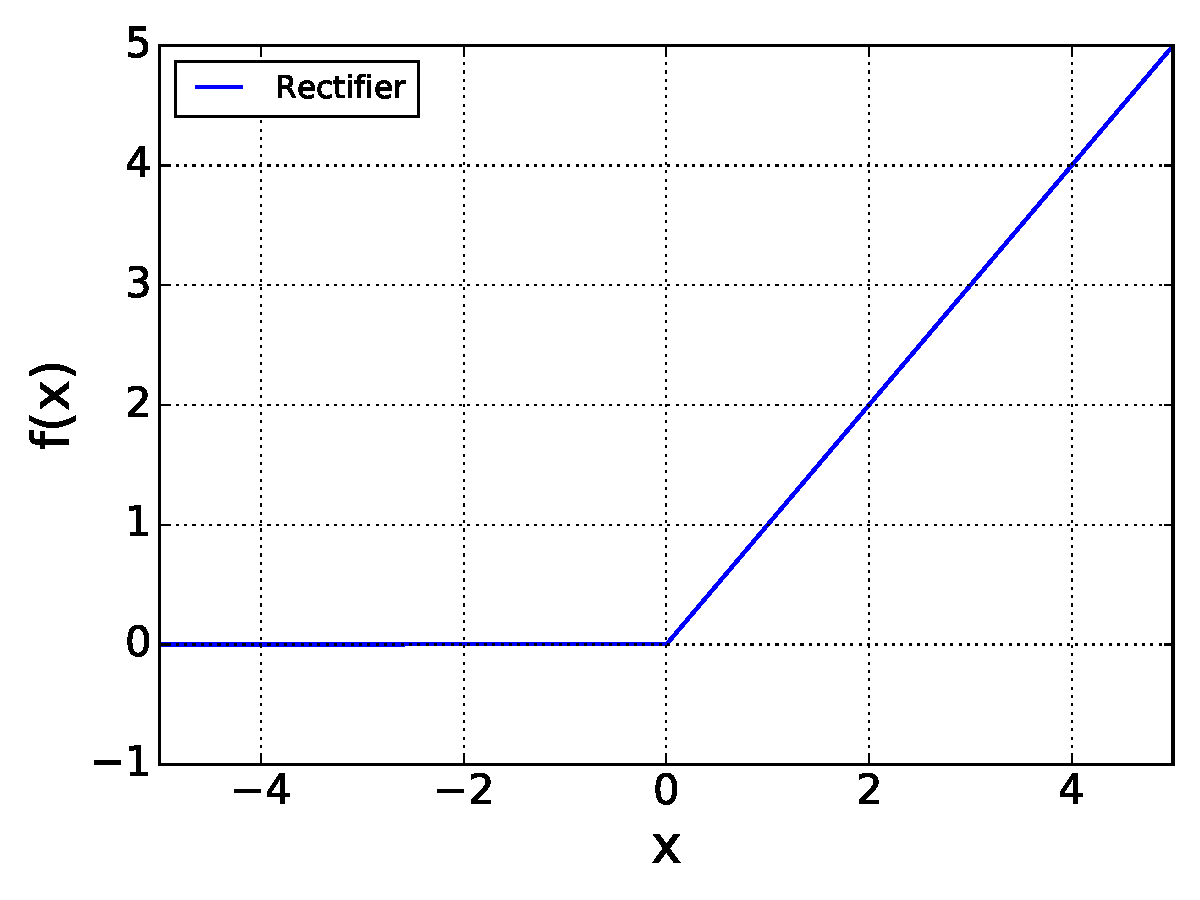
\includegraphics[width = 0.7\linewidth]{Figures/Theory/reluActivation.pdf}
  \caption{Two of the most common activation functions for neural networks. Both meet the requirements
	   of the universal approximation theorem.}
  \label{fig:reluActivationFunction}
  \end{center}
\end{figure}


\section{Training} \label{sec:training}
In the beginning of this chapter we defined machine learning as the ''science of giving computers the ability to learn without
being explicitly programmed.'' In the neural network case, this learning is achieved by iteratively adjusting 
the parameters, i.e. the weights and biases (in the following, ''weights'' will often be equivalent to all 
the NN parameters, including the biases).
The procedure depends on what learning paradigm we work with
(unsupervised or supervised learning), and the type of NN we use. 

In this thesis we employ NNs for regression: we want to interpolate data sets og atomic coordinates and energies.
The goal is to adjust the weights of a MLP so that it accurately represents a function that maps
atomic coordinates to the corresponding energies. Interpolation with NNs is essentialy an optimization problem:
the weights are typically initialized as random numbers, and then modified iteratively to minimize the error
to a set of expected output values, in our case energies. 
This procedure is called \textit{training}. 

The input values to the function that we want to fit
are called the \textit{training set}, while the output values are called the \textit{reference set} or the \textit{target values}.
The training set $X$ and reference set $Y$ are represented as matrices, where the $i$-th row of $X$ and $Y$, 
denoted $X_{i*}$ and $Y_{i*}$ respectively, 
together form a \textit{training example}. The combined data set consists of $N$ such training examples. 
Note that the number of columns of $X$ and $Y$ are equal to the number of inputs and outputs of our MLP respectively. 
This is a restatement of the observation made in \autoref{sec:MLPmodel}: the number of inputs and outputs of our MLP must be equal 
to the number of input and output values of the function we are trying to fit. 


\subsection{Cost functions} \label{costFunctions}
To minimize the error, we need a way to \textit{define} it. 
As in mathematical optimization, the error is represented by an objective function, also called \textit{loss} function
or \textit{cost} function. Training a NN therefore amounts to the minimization of this function, which can be written in the 
following general way,
\begin{equation}
 \Gamma = \Gamma(W, B, X, Y)
 \label{generalCost}
\end{equation}
where $W$ and $B$ are the NN's weights and biases respectively. 
The value of this function is a measure of how well the NN is able to map $X \rightarrow Y$. 
By adjusting $W$ and $B$, we try to minimize the value of this function.  

The standard cost function used in regression with NNs is the mean-square error,
\begin{equation}
 \Gamma = \frac{1}{2N}\sum_{i=1}^N (Y_i - y_i)^2
 \label{quadraticCost}
\end{equation}
where $y_i = y_i(W, B, X_{i*})$ is the value predicted by the NN for traing example $X_{i*}$. 
For a MLP with more than one output, $Y_i$ and $y_i$ are vectors. 
The constant $1/2$ is included to cancel out the exponent when this function is differentiated in \autoref{sec:backprop}.

A variety of other cost functions are used for other machine learning tasks. In classificiation the output is often binary, 
hence the mean-square error function is inadequate. We will not go into further detail on other cost functions here. 


\section{Optimization} \label{sec:optimization}
There are a large number of algorithms that can be used to determine the set of weights minimizing the 
cost function \eqref{quadraticCost}. 
Different kinds of gradient descent-based methods are widely used, while higher order methods like
the conjugate gradient algorithm or Newton's method are rarely seen in the literature because they are 
too computationally expensive for large NNs and data sets. Therefore, only first-order methods will be discussed here. 

The idea behind gradient descent methods is to minimize a function by 
iteratively taking steps in the direction of steepest descent towards a minima in parameter space. 
This direction is defined as the negative gradient of the function w.r.t. 
all its parameters. If we define $\vec{\theta} \in \mathbb{R}^d$ as a vector containing all the weights and biases
of a MLP, we get the following iterative scheme,
\begin{equation}
 \vec{\theta}_{k+1} = \vec{\theta}_{k} - \gamma \nabla_{\vec{\theta}_k} \Gamma(\vec{\theta})
 \label{gradientDescent}
\end{equation}
where $\gamma$ is a step size, called the \textit{learning rate} in the context of machine learning. The process is started
by initializing the parameters as random numbers. The value of $\gamma$ is of great importance for the algorithm to converge,
and is allowed to change at every iteration. Note that convergence to 
a minimum is not guaranteed withouth certain assumptions on the function $\Gamma$ and the particular choices of $\gamma$.
Also, the obatained minimum is generally local, not global. 
Different ways to update $\gamma$ is discussed below.


\subsection{Gradient descent variants} \label{gradientDescentVariants}
There are three versions of gradient descent \cite{Ruder16}, which differ in 
the number of training examples we present to the NN before updating the parameters. 
According to neural network terminology, the process of adjusting the parameters based on all the training examples,
either in batches or all at once, is called an \textit{epoch}. 

In \textit{batch} gradient descent, 
we compute the gradient of the cost function for the \textit{whole} training set before updating, also called 
\textit{offline learning}. 
This approach can be very slow and is intractable for datasets that do not fit in memory. Furthermore, there is a risk
of performing redundant computations if many similar examples are present in the data set.

In contrast, \textit{stochastic} gradient descent (SDG) performs a parameter update for \textit{each} training example. 
SDG avoids redundant gradient calculations and is therefore faster than batch gradient descent. However, the accuracy 
of each update is lower, which can lead to quite large error oscillations. The concept of having  
more than one parameter update per epoch is called \textit{online learning}. 

Finally, we have \textit{mini-batch} gradient descent, which is a mix of the two other approaches. The training set 
is divided into $n$ equally sized mini-batches and a parameter update is performed for each mini-batch. This is usually the
algorithm of choice, as it has the optimal trade-off between speed and accuracy. Normal mini-batch sizes range
between 50 and 256, but should in some degree be tailored to each problem. 

We realize that SDG can be seen as 
a variant of mini-batch gradient descent with a mini-batch size of 1. In the literature, these two methods 
are often collectively referred to as SDG. We will adopt this naming convention for the rest of this thesis. 


\subsection{Optimization algorithms} \label{sec:optimizationAlgorithms}
In the following we will outline different optimization algorithms that are widely used in neural network research. 
They are all variations on the update rule \eqref{gradientDescent}. The main focus of the methods is to find
a proper learning rate. A learning rate that is too small may lead to very slow convergence, while 
a learning rate that is too large can cause the loss function to fluctuate around the minimum or even diverge. 

\subsubsection{Momentum}
Near local minima, the surface area of the cost function (in parameter space) often curve much more steeply in one 
direction than in another, forming ravines. SDG will have slow converge in such regions, as it will oscillate across the slopes
while having slow progress along the bottom of the ravine. The Momentum method \cite{Qian99} avoids this problem
by accelerating SDG in the downwards direction, while damping the oscillations. The update rule is
\begin{equation}
\begin{aligned}
 \vec{v}_{k} &= \eta \vec{v}_{k-1} + \gamma \nabla_k \Gamma \\
 \vec{\theta}_{k+1} &= \vec{\theta}_k - \vec{v}_k
\end{aligned}
\label{Momentum}
\end{equation}
where $\eta$ is the momentum term, which is usually set to 0.9 or a similar value. The new update vector $\vec{v}_k$ 
is formed by adding a fraction $\eta$ of the previous update vector $\vec{v}_{k-1}$ to the gradient. In this way, the magnitude
of the update decreases for parameters (dimensions) whose gradients change direction, while it increases for parameters
whose gradients points in the same direction as in the previous step. This helps to push SDG downhill towards the minima. 

\subsubsection{Adagrad}
In SDG and Momentum, we have one learning rate $\gamma$ that is applied to all the parameters. 
Ideally, the learning rate should be adapted to each individual parameter to perform larger or smaller updates
depending on their importance. Adagrad \cite{Duchi11} does just that. For brevity, we set
\begin{equation}
 g_{k,i} = \nabla_{\theta_i} \Gamma (\vec{\theta})
\end{equation}
to be the gradient of the loss function w.r.t. parameter $\theta_i$ at step $k$. Adagrad adjust the general learning rate $\gamma$
at each step $k$ for every parameter $\theta_i$ based on the past gradients for that parameter,
\begin{equation}
 \theta_{k+1,i} = \theta_{k,i} - \frac{\gamma}{\sqrt{G_{k,ii} + \epsilon}} \cdot g_{k,i}
\end{equation}
where $G_k \in \mathbb{R}^{d \times d}$ is a diagonal matrix where each diagonal element $G_{k,ii}$ is the sum of squares
of the gradient w.r.t. $\theta_i$ up to step $k$. The smoothing constant $\epsilon \sim 10^{-8}$ is present to avoid
division by zero. This vectorized version of this equation yields,
\begin{equation}
  \vec{\theta}_{k+1} = \vec{\theta}_k - \frac{\gamma}{\sqrt{\mathrm{diag}(G_k) + \epsilon}} \odot \vec{g}_k
  \label{Adagrad}
\end{equation}
where $\odot$ stands for element-wise multiplication. In other words, we do not have to manually tune the learning rate, 
Adagrad does that for us. A weakness of this method is that the learning rates inevitably shrink for each step, 
resulting in arbitrary small values, at which point the learning stops.

For the rest of \autoref{sec:optimizationAlgorithms}, we assume for brevity that all vector operations are element-wise, i.e.
$\vec{g}\,\vec{h} = \vec{g} \odot \vec{h}$ and $\vec{g}^2 = \vec{g} \odot \vec{g}$.

\subsubsection{Adadelta}
Adadelta \cite{Zeiler12} is an extension of Adagrad that reduces the rate at which the learning rate decreases. 
The sum of all past squared gradients is replaced by a \textit{exponentially decaying average} of all the previous squared gradients.
We introduce the vector $\mathrm{E}[\vec{g}^2]_k$ containing the decaying averages of the gradient w.r.t. all the parameters at step $k$. 
This vector is defined recursively
as a weighted average of the previous averages $\mathrm{E}[\vec{g}^2]_{k-1}$ and the current gradient $\vec{g}_k$,
\begin{equation}
 \mathrm{E}[\vec{g}^2]_k = \eta \mathrm{E}[\vec{g}^2]_{k-1} + (1 - \eta) \vec{g}^2_k
 \label{decayingAverageVector}
\end{equation}
where $\eta$ is a decay constant similar to that in the Momentum method, and is usually set to the same value (0.9). 
We also define a new parameter update vector $\Delta \vec{\theta}_k = -\vec{v}_k$ so that
\begin{equation}
 \vec{\theta}_{k+1} = \vec{\theta}_k  + \Delta \vec{\theta}_k
\end{equation}
Replacing the vector $\mathrm{diag}(G_k)$ in \eqref{Adagrad} with the decaying average vector \eqref{decayingAverageVector}
yields the following parameter update vector,
\begin{equation}
 \Delta \vec{\theta}_k = -\frac{\gamma}{\sqrt{\mathrm{E}[\vec{g}^2]_k + \epsilon}} \vec{g}_k
 \label{preliminiaryAdadelta}
\end{equation}
Additionally, the learning rate $\gamma$ is replaced by a decaying average of previous squared parameter updates
up to step $k-1$, yielding the Adadelta update rule,
\begin{equation}
 \vec{v}_k = \frac{\sqrt{\mathrm{E}[\Delta\vec{\theta}^2]_{k-1} + \epsilon}}{\sqrt{\mathrm{E}[\vec{g}^2]_k + \epsilon}} \vec{g}_k
\end{equation}
The final replacement is done to obtain correct units for the update vector and to eliminate the learning rate from the equation. 
Thus, we do not even need to set a default learning rate with Adadelta. 

\subsubsection{Adam}
The final algorithm we are going to discuss is Adapte Moment Estimation (Adam) \cite{Kingma14}. This method
computes adaptive learning rates for each parameter by storing 
exponentially decaying averages of both the gradients \textit{and} 
the squared gradients \eqref{decayingAverageVector},
\begin{equation}
 \begin{aligned}
  \mathrm{E}[\vec{g}]_k &= \beta_1 \mathrm{E}[\vec{g}]_{k-1} + (1 - \beta_1) \vec{g}_k \\
  \mathrm{E}[\vec{g}^2]_k &= \beta_2  \mathrm{E}[\vec{g}^2]_{k-1} + (1 - \beta_2) \vec{g}^2_k
 \end{aligned}
\end{equation}
We set $\vec{a}_k = \mathrm{E}[\vec{g}]_k$ and $\vec{b}_k = \mathrm{E}[\vec{g}^2]_k$ so that
\begin{equation}
 \begin{aligned}
 \vec{a}_k &= \beta_1 \vec{a}_{k-1} + (1 - \beta_1) \vec{g}_k \\
 \vec{b}_k &= \beta_2 \vec{b}_{k-1} + (1 - \beta_2) \vec{g}^2_k
 \end{aligned}
\end{equation}
where $\vec{a}_k$ and $\vec{b}_k$ are estimates of the first moment (the mean) and the second moment (the uncentered variance)
of the gradients respectively, hence the name of the method. The elements of these two vectors are initialized as zeros, 
which make them biased towards zero, especially during the first time steps. This bias is counteracted by
computing bias-corrected version of the vectors (derived in \cite{Kingma14},
\begin{equation}
 \begin{aligned}
 \hat{\vec{a}}_k &= \frac{\vec{a}_k}{1 - \beta_1^k} \\
 \hat{\vec{b}}_k &= \frac{\vec{b}_k}{1 - \beta_2^k}
 \end{aligned}
\end{equation}
The parameter update vector for Adam is obtained by replacing the gradient $\vec{g}_k$ with $\vec{a}_k$ in \eqref{preliminiaryAdadelta},
yielding the update rule,
\begin{equation}
 \vec{\theta}_{k+1} = \vec{\theta}_k - \frac{\gamma}{\sqrt{\hat{\vec{b}}_k} + \epsilon} \hat{\vec{a}}_k
\end{equation}
The default values of the hyperparameters are $\beta_1 = 0.9$, $\beta_2 = 0.999$ and $\epsilon = 10^{-8}$. 

\subsubsection{Which optimizer to use?}
There is no general answer to the question stated above. The adaptive learning rate methods
like Adagrad, Adadelta and Adam are generally more robust because they do not rely on manual fine-tuning of the learning rate. 
Also, an adaptive learning rate generally handles \textit{sparse} data better, i.e. data where some learning features
are poorly represented. 

Adam has been proven to perform favourably over the other optimization methods for certain applications like classification
with MLPs and convolutional NNs \cite{Kingma14}. However, the performance of various optimizers should be tested on 
the problem at hand to determine which method that works best. 




\subsection{Backpropagation} \label{sec:backprop}
From: https://www.willamette.edu/~gorr/classes/cs449/backprop.html and \newline
http://neuralnetworksanddeeplearning.com/chap2.html. 
Mainly from the first one, but argument for error of neuron from second.

In the preceding sections we have discussed different optimizers that implements various update rules for 
the parameters of a loss function. In our case, these parameters are the weights and biases of a neural network
and the cost function $\Gamma$ is the mean-square-error \eqref{quadraticCost}
\begin{equation}
 \Gamma = \frac{1}{2} (Y - y)^2
\end{equation}
here written as a function of only \textit{one} training example. 
What we have not discussed yet, is
how we calculate the gradient of the cost function, i.e. how we obtain the partial derivatives $g_{ij}$ and $h_i$ w.r.t.
all the weights and biases respectively,
\begin{equation}
\begin{aligned}
 g_{ij} &= \frac{\partial \Gamma}{\partial w_{ij}} \\
 h_i &= \frac{\partial \Gamma}{\partial b_i}
\label{partialDerivatives}
\end{aligned}
\end{equation}
where we have dropped layer indicies for clarity. 
A common method to obtain these derivatives is \textit{backpropagation} \cite{Rumelhart86}. 
In backpropagation, a training example is propagated forward through the NN to produce an output. 
This output is compared to the desired output (target values), and the error is then propagated \textit{backwards}
through the layers to obtain the amount of which each parameter should be adjusted, 
hence the name.
The method is essentially an implementation of the chain rule, and will allow us to calculate
the partial derivatives of the cost with respect to all the parameters, thereby obtaining the gradient of the network. 

\subsubsection{1. Forward propagation}
The first stage of the algorithm is forward propagation, producing an output as described in \autoref{sec:MLPmodel}.
\footnote{We assume that the MLP only has one output. As before, the results are valid for each individual output in 
a many-output MLP.}
In the following, we will use the same notation as in \autoref{sec:MLPmodel}. We also define
\begin{equation}
 A_i = \{j:w_{ij}\}
\end{equation}
as the set $\{j\}$ of nodes anterior to node $i$ and connected to node $i$ with weights $w_{ij}$, in addition to
\begin{equation}
 P_j = \{i:w_{ij}\}
\end{equation}
as the set $\{i\}$ of nodes posterior to node $j$ and connected to node $j$ with weights $w_{ij}$. 

\subsubsection{2. Backward propagation}
The second step is to backpropagate the error of the NN output. The weight derivative \eqref{partialDerivatives}
can be expanded into two factors by use of the chain rule,
\begin{equation}
 g_{ij} = \frac{\partial \Gamma}{\partial u_i}\frac{\partial u_i}{\partial w_{ij}}
 \label{partialDerivativeExpanded}
\end{equation}
Now we move in the opposite direction of the feed-forward stage: First we differentiate the cost w.r.t 
the input of neuron $i$, then we differentiate the input w.r.t. weight $w_{ij}$ connecting neurons $j$ (in the preceding layer)
and $i$. 
The first term on the r.h.s. is defined as the the error $\delta_i$ of node $i$, 
\begin{equation}
 \delta_i = \frac{\partial\Gamma}{\partial u_i}
 \label{neuronError}
\end{equation}
This definition can be justified by the following argument.
To change the value of a cost function \eqref{generalCost}, we need to change the outputs of the neurons in the network. 
Changing the input $u_j$ to neuron $j$ by a small amount $\Delta u_j$ results in the output
\begin{equation}
 y_j = f_j(u_j + \Delta u_j)
\end{equation}
This change will propagate through later layers in the network, finally causing the overall cost to change
by an amount $\frac{\partial \Gamma}{\partial u_j}\Delta u_j$. If $\partial \Gamma / \partial u_j$ is close to zero,
we are not able improve the cost much by perturbing the weighted input $u_j$; the neuron is already quite near the optimal value.
This is a heuristic argument for $\partial \Gamma / \partial x_j$ to be a measure of the error of the neuron. 

\noindent The second term on the r.h.s. of \eqref{partialDerivativeExpanded} is 
\begin{equation}
 \frac{\partial u_i}{\partial w_{ij}} = \frac{\partial}{\partial w_{ij}} \sum_{m\in A_i} w_{im}y_m = y_j
 \label{derivativeSecondTerm}
\end{equation}
Combining the the two terms \eqref{neuronError} and \eqref{derivativeSecondTerm} yields
\begin{equation}
 g_{ij} = \delta_i y_j
 \label{weightGradient}
\end{equation}
To compute this quantity, we thus need to know the outputs and the errors of all nodes in the network. 
The outputs are generated during the feed-forward stage \eqref{generalLayer},
\begin{equation}
 y_i = f_i(u_i) = f_i\left(\sum_{j\in A_i} w_{ij}y_j + b_i\right)
 \label{forwardProp}
\end{equation}
and need to be stored for all nodes. 
The errors are obtained by backpropagating the error of the output neuron $o$,
\begin{equation}
 \delta_o = \frac{\partial \Gamma}{\partial u_o} = \frac{\partial \Gamma}{\partial y_o}\frac{\partial y_o}{\partial u_o}
          = (Y - y_o) \frac{\partial y_o}{\partial u_o}
\end{equation}
We remember from \autoref{sec:MLPmodel} that the output neuron has the identity activation function $y_o = f_o(u_o) = u_o$, 
which reduces the error to
\begin{equation}
 \delta_o = Y  - y_o
\end{equation}
This error is then propagated backwards through the network, layer by layer. 
The error of each neuron in layer $l$ thus depends on the errors of all nerons in layer $l+1$.  
Consequentially, the error of an arbitrary hidden neuron can be written as a recursive equation (\autoref{fig:backprop}),
\begin{equation}
 \delta_j = \frac{\partial \Gamma}{\partial u_j} = 
 \sum_{i\in P_j} \frac{\partial \Gamma}{\partial u_i}\frac{\partial u_i}{\partial y_j}\frac{\partial y_j}{\partial u_j}
 \label{errorTerms}
\end{equation}
\begin{figure}
\begin{center}
 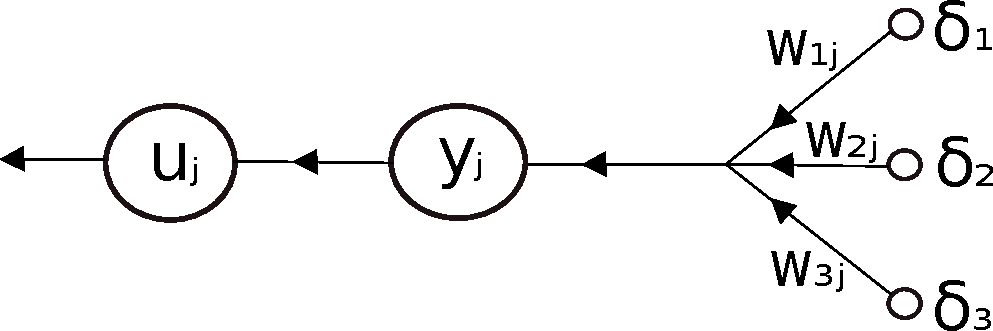
\includegraphics[width = 0.9\linewidth]{Figures/Theory/backprop.pdf}
  \caption{Illustration of the backpropagation algorithm. The direction of information flow is opposite of \autoref{fig:neuronModel}. 
	   A hidden neuron $j$ recieves a weighted sum of errors of all nodes in the posterior layer. Then, we differentiate
	   in the backwards direction: the activation function (output) $y_j$ of node $j$ is differentiated w.r.t to its 
	   net input $u_j$.}
  \label{fig:backprop}
  \end{center}
\end{figure}
We observe that also the inputs $u_i$ to all nodes need to be stored during forward propagation for 
this scheme to work. 
The first term on the r.h.s. of \eqref{errorTerms} is the error $\delta_i$ of node $i$, which is assumed to be known. 
As long as there are no cycles in the network, there is an ordering
of nodes from the output back to the input that respects this condition. It is
therefore valid only for feed-forward NNs.

The second term is the derivative of the net input of all posterior
nodes $\{i\}$ w.r.t. the output of node $j$,
\begin{equation}
 \frac{\partial u_i}{\partial y_j} = \frac{\partial}{y_j}\left(\sum_{m\in A_i} w_{im}y_m + b_i\right) = w_{ij}
\end{equation}
while the third is the derivative of node $j$'s activation function w.r.t. its net input:
\begin{equation}
 \frac{\partial y_j}{\partial u_j} = \frac{\partial f_j(u_j)}{\partial u_j} \equiv y^\prime_j
\end{equation}
Putting all the pieces together we obtain
\begin{equation}
 \delta_j = y^\prime_j\sum_{i\in P_j}w_{ij} \delta_i 
 \label{backprop}
\end{equation}
This expression is illustrated in \autoref{fig:backprop}.  
Each hidden neuron $j$ recieves a weighted sum
of the errors of all nodes in the posterior layer. Then we differentiate in the backwards direction (compare with 
\autoref{fig:neuronModel}): 
the output $y_j$ of node $j$ is differentiated w.r.t. its input $u_j$. 

The errors are propagated backwards through the whole NN until we reach the weights connecting the input layer
and the first hidden layer. 
By propagating the error
of only one ouput neuron, we thus obtain the errors of all the neurons at once. This is the main strength of the backpropagation
algorithm, and the reason for its popularity in neural network research. 

\noindent For the biases, we have \eqref{partialDerivatives},
\begin{equation}
 h_j = \frac{\partial \Gamma}{\partial b_j} = \sum_{i\in P_j} \frac{\partial \Gamma}{\partial u_i}
	      \frac{\partial u_i}{\partial y_j} \frac{\partial y_j}{\partial u_j} \frac{\partial u_j}{\partial b_j}
\end{equation}
The only new term her is the last one:
\begin{equation}
 \frac{\partial u_j}{\partial b_j} = \frac{\partial}{\partial b_j}\left(\sum_{m\in A_j} w_{jm}y_m + b_j\right) = 1
\end{equation}
Consequentially, the bias gradient is simply the error of each neuron:
\begin{equation}
 h_j = \delta_j
\end{equation}

\subsubsection{Matrix notation}
In \autoref{sec:MLPmodel} we rewrote the forward propagation framework as matrix-vector equations. 
This is easily done also for the backpropagation case. From \autoref{sec:MLPmodel} we have the
set of vectors $\vec{b}^l$ and $\vec{y}^l$ for $l = 1,\dots ,L+1$, 
where $L$ is the number of hidden layers. We now extend this set with the vectors $\vec{\delta}^l$ 
and $\vec{u}^l$, i.e. the errors and inputs (or \textit{preactivations}) of layer $l$
respectively. These are all column vectors of size $N_l \times 1$. 

\noindent Comparing the sums in \eqref{forwardProp} and \eqref{backprop}, we realize that since 
\begin{equation}
 \sum_j w_{ij} y_j \: \Rightarrow \: W \vec{y}
\end{equation}
we have
\begin{equation}
  \sum_i w_{ij} \delta_i \:  \Rightarrow \: W^T \vec{\delta}
\end{equation}
i.e. the weight matrices used in backpropagation are the transpose of the matrices used in forward activation.
Thus, for nodes $\{j\}$ in layer $l$ and nodes $\{i\}$ in layer $l+1$, the vectorized equation for the error of each hidden neuron is
\begin{equation}
 \delta_j = y^\prime_j\sum_{i\in P_j}w_{ij} \delta_i \: \Rightarrow \:
 \vec{\delta}_l = \vec{y}^\prime_l \odot (W_{l+1} \vec{\delta}_{l+1})
\end{equation}
where $\odot$ signifies element-wise multiplication. The expression for the weight gradients \eqref{weightGradient} is converted
into an outer product of the errors of layer $l+1$ and the outputs of layer $l$,
\begin{equation}
 g_{ij} = \delta_i y_j \Rightarrow G_l = \vec{\delta}_{l+1} \vec{y}^T_l
\end{equation}
where $G_l$ is a matrix containing all gradients for the weights connecting layer $l$ and $l+1$. 
The corresponding matrix for the biases is a $N_l \times 1$ column vector $\vec{H}_l$,
\begin{equation}
 \vec{H}_l = \vec{\delta}_l
\end{equation}
The set $\{G_l, \vec{H}_l\}$ for $l=1,\dots,L+1$ thus make up the total gradient of the cost function \eqref{quadraticCost}. 

\subsubsection{Training algorithm}
We are now ready to express the complete training algorithm for a MLP with backpropagation using
matrix-vector notation. The below process is performed for each training example $\vec{x} = X_{i*}$ in the whole
training set.
\begin{enumerate}
 \item Initialize the input layer:
 \begin{equation}
  \vec{y}_0 = \vec{x}
 \end{equation}
 \item Propagate the activity forward: for $l = 1,\dots,L+1$:
 \begin{equation}
 \begin{aligned}
  \vec{u}_l &= W_l\vec{y}_{l-1} + \vec{b}_l \\
  \vec{y}_l &= f_l(\vec{u}_l)
  \label{forwardPropMatrix}
 \end{aligned}
 \end{equation}
 Store all vectors $\vec{u}_l$ and $\vec{y}_l$.
 \item Calculate the error in the output layer:
 \begin{equation}
  \vec{\delta}_{L+1} = \vec{Y} - \vec{y}_{L+1}
 \end{equation}
 \item Backpropagate the error: for $l = L, L-1, \dots ,1$:
 \begin{equation}
 \vec{\delta}_l = \vec{y}^\prime_l \odot (W^T_{l+1}\vec{\delta}_{l+1}) \cdot 
 \label{backPropMatrix}
 \end{equation}
 Store all errors $\vec{\delta}_l$. 
 \item Compute weight and bias gradients: 
 \begin{equation}
  G_l = \vec{\delta}_l \vec{y}_{l-1}^T, \quad \vec{H}_l = \vec{\delta}_l
 \end{equation}
 \item Update weights and biases using an update rule of choice
\end{enumerate}


\chapter{Neural networks in molecular dynamics} \label{sec:NNsAndMD}
In \autoref{sec:constructingPES} we discussed various ways to construct a PES for use in molecular dynamics, and
stated that this thesis deales with neural network potentials (NNP). Then, in \autoref{sec:machineLearning}
we outlined the basic theory of MLPs, which is our choice of neural network type. In this chapter, 
we discuss the pros and cons of NNPs, and different properties such potentials should possess to 
fulfill important physical symmetries. 

\section{Neural network potentials}
NNPs are constructed by fitting an analytic function to a set of reference data
obtained by quantum mechanical calulations.
The main goal of the NN approach to constructing a PES, is to create a potential that has the accuracy of \textit{ab inito}
methods and the speed of empirical potentials (or at least of the same order).

Several different methods have been developed to construct NNPs. A comprehensive review of many of these 
was written by Behler in 2011 \cite{Behler11general}. They mainly differ in the number of NNs that are employed 
to represent the total energy of the system, the dimensionality of each NN and the choice of input coordinates. 
By dimensionality we mean the number of input nodes, as the number of output nodes is assumed to be 1 if not specified otherwise. 

\subsection{Potentials using single neural network}
In the literature, the dominant part of NN potentials employ a single feed-forward NN to calculate the total energy of the system.
This is the most straightforward approach and is the easiest to implement.
For instance, Agrawal et al. \cite{Agrawal06} have used a single, three-dimensional NN to study the dissociation of the 
$\mathrm{SiO}_2$ molecule. However, these types of NNPs suffer from a number of limitations. Most importantly, 
they have a fixed dimensionality. This is a general property of FFNNs where the atomic coordinates are fed directly 
to the network without any transformations: once fitted, the NNP can only be applied to systems with the same number of atoms
as the number of inputs. Further, a large number of input nodes requires many hidden neurons, and there comes a point 
where the number of parameters of the NN makes training unfeasible. Thus, the number of degrees of freedom of the system 
must be small. 

\subsection{Potentials using multiple neural networks}
For NNPs to be recognized as competitive potentials in molecular dynamics, they should be applicable to large systems
of various sizes, containing thousands of atoms. This can not be achieved by employing only one NN to 
represent the total energy of the system. A solution is to replace the single NN by a set of \textit{atomic} NNs, where 
each NN provides the contribution $E_i$ of \textit{one} atom to the total energy $E_s$ of the system, 
\begin{equation}
 E_s = \sum_{i=1}^N E_i
 \label{systemEnergy}
\end{equation}
Two methods using this approach have been developed in parallel by Bholoa et al. \cite{Bholoa07}, and Behler and Parinello 
\cite{Behler07}.
Both methods compute $E_i$ based on the chemical environment of atom $i$, but they differ in how 
the environment is represented and also how the atomic NNs are structured. 

Bholoa et al. compute each atomic energy $E_i$ by a NN of variable size, using a set of 
vectors as input to the NN. Each vector specifies the geometry of a four atom chain $i-j-k-l$ describing the chemical 
environment. The input layer and first hidden layer are replicated once for each vector, thus the problem 
of fixed dimensionality is solved. 

Behler and Parinello have developed a different approach to constructing a NNP. 
We have chosen to use the Behler-Parinello (BP) method in this thesis, and this will be the topic of the 
rest of the chapter. 

\section{The Behler-Parinello method}
In the Behler-Parinello (BP) method, the architecture of each NN is fixed, and
the atomic energies $E_i$ depend on the local chemical environments up to a cutoff radius $R_c$. 
This is analogous to the introduction of a cutoff radius in MD simulations
(\autoref{sec:forceCutoff}). Thus, the NNP can be applied to MD simlulations in excactly the same way 
as ordinary, empirical potentials: it is simply an analytic function that yields the potential energy of a central atom
in the presence of neighbouring atoms contained in a cutoff sphere of radius $R_c$. 
In other words, the BP method employs an \textit{atom-centered} approach. 
In the following we will refer to all atoms inside the cutoff sphere of an atom $i$ as \textit{neighbours}.

The cutoff is introduced by a set of so-called symmetry functions. 
These functions
describe the local chemical environment of an atom $i$ by transforming the cartesian coordinates of \textit{all} its neighbours to 
a predefined number of function values, forming a symmetry vector. 
The symmetry vector is used as input to the atomic NN of atom $i$, that in turn calculates its potential energy $E_i$.
The length of this vector must therefore be equal to the number of NN inputs. 

Each atom has an individual atomic NN along with a fixed set of symmetry functions, but
all atoms of the same element have identical 
atomic NNs and symmetry functions sets. Thus, for a diatomic system, only two unique NNs need to be trained. 

As an example, let us look at a system containing two different elements: Si and O. 
All Si atoms have idential atomic NNs and symmetry function sets, the former represented by the function $F_{\mathrm{Si}}$. 
A given Si atom $i$ has at a given time $n$ neighbours, including both Si and O atoms.  
We define $\vec{R}_{ij} = (r_{i1}, r_{i2}, \dots, r_{in})$ as the vector containing the distances from
atom $i$ to all neighbours $j = 1,\dots,n$, where $r_{ij} = |\vec{r}_j - \vec{r}_i|$. 
Further, $\vec{G}_\mathrm{Si}(\vec{R}_{ij}) = \{G_{\mathrm{Si},s}(\vec{R}_{ij})\}$ is the vector of Si symmetry functions
$s = 1,\dots,M_\mathrm{Si}$. \footnote{This notation signifies that each symmetry function, i.e. each element of 
the symmetry vector, depends on the coordinates of all atoms in the cutoff sphere. However, it does not say anything about
the form of the dependence, e.g. if it involves triplets or just pairs of atoms etc.}
The process of calculating the potential energy $E_i$ described above can then be written,
\begin{equation}
 \vec{R}_{ij} \rightarrow \vec{G}_\mathrm{Si}(\vec{R}_{ij}) \rightarrow F_\mathrm{Si}[\vec{G}_\mathrm{Si}(\vec{R}_{ij})] 
 \rightarrow E_i
 \label{BPatomicEnergySi}
\end{equation}
To obtain the corresponding expression for an O atom, we simply substitute $\mathrm{Si} \rightarrow \mathrm{O}$. 
The expression is valid for any element e, and for a system with an arbitrary number of elements,
\begin{equation}
  \vec{R}_{ij} \rightarrow \vec{G}_\mathrm{e}(\vec{R}_{ij}) \rightarrow F_\mathrm{e}[\vec{G}_\mathrm{e}(\vec{R}_{ij})] 
 \rightarrow E_i
 \label{BPatomicEnergy}
\end{equation}
While the symmetry function vector of an element e is of a fixed size equal to the number of inputs to $F_\mathrm{e}$,
the length of $\vec{R}_{ij}$ can be arbitrary. This is enabled by the functional form of the symmetry functions, 
which is the topic of the next section. 

We note that although the NNs and the symmetry vectors
are identical for all atoms of the same element, the resulting energies $E_i$ are not equal since 
they depend on the unique atomic environments $\vec{R}_{ij}$ of each atom. 




\subsection{Symmetry functions} \label{sec:symmetryFunctions}
We have mentioned two requirements that the symmetry function set have to meet. First, they must contain a cutoff $R_c$
that defines a chemical environment. Secondly, since we employ atomic NNs with a fixed number of inputs,
they have to be able to produce a constant 
number of function values independent of the number of neighbours, which can change during MD simulations. 

In addition to this, the NN has a symmetry problem. It does not take into account that exchanging two or more atoms
can lead to an energetically equivalent configuration. For example, exchanging the positions of both hydrogen atoms
in a water molecule will not alter the energy. However, noting that all weights have numerically different values,
changing the order of the input coordinates to the NN will result in a different energy value. This problem can be solved
by employing symmetry functions that are invariant with respect to the order of the atoms.  

We start with defining the chemical environments by introducing a cutoff funciton \cite{Behler11symmetry},
\begin{equation}
 f_c(R_{ij}) = 
\begin{cases}
0.5 \cdot \left[\cos\left(\frac{\pi R_{ij}}{R_c}\right) + 1 \right], & R_{ij} \leq R_c \\
0, & R_{ij} > R_c
\end{cases}
\label{cutoffFunction}
\end{equation}
which is the monotonically decreasing part of a cosine function on $R_{ij} \in [0,R_c]$ (\autoref{fig:cutoffFunction}). 
\begin{figure}[h]
\begin{center}
  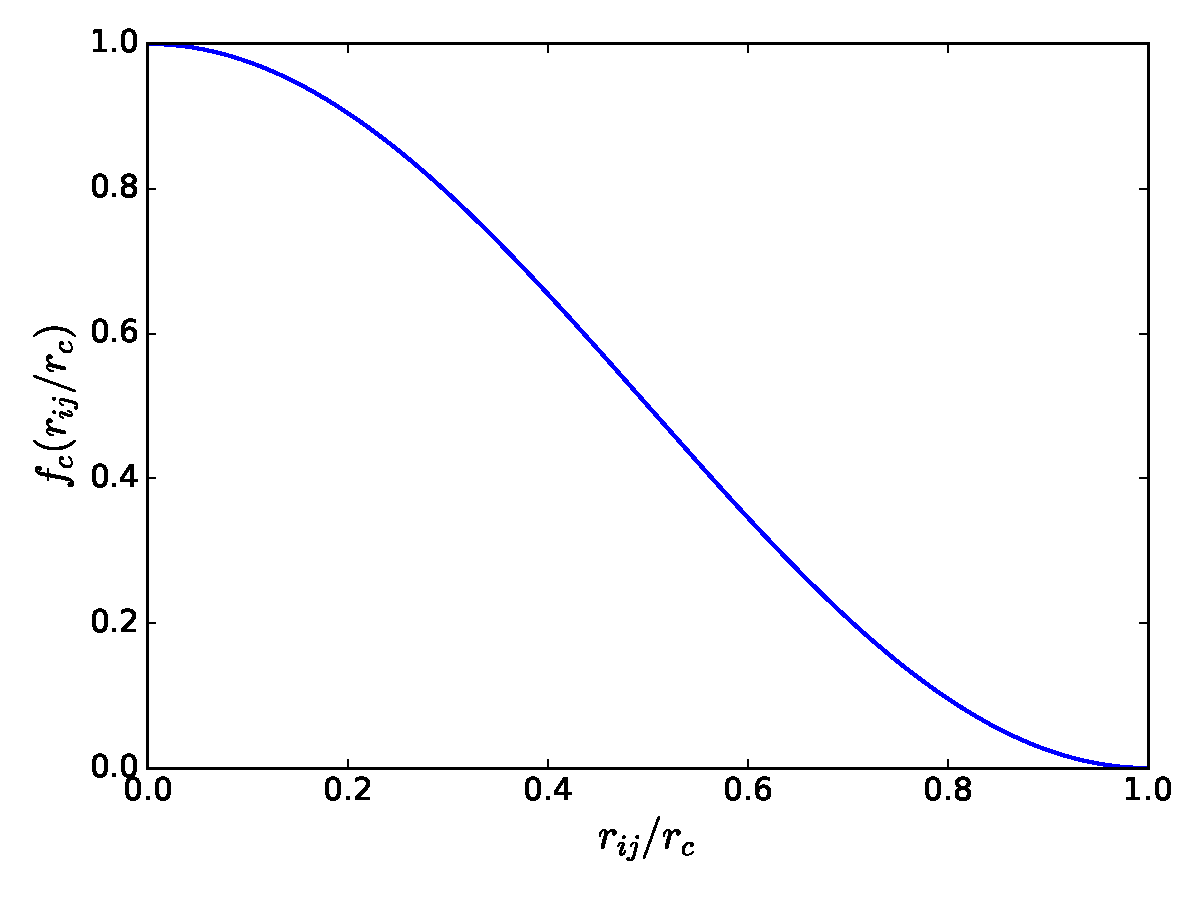
\includegraphics[width = 0.9\linewidth]{Figures/Theory/cutoffFunction.pdf}
  \caption{Plot of the cutoff function \eqref{cutoffFunction} applied in this thesis. 
	   This function is used to define a chemical environment around a central atom:
           only the atoms within the cutoff radius $R_c$ contribute to its energy. 
           These are called neighbouring atoms. The closer a neighbouring atom is, the larger
           the energy contribution, as is the case for most physical systems.}
  \label{fig:cutoffFunction}
  \end{center}
\end{figure}
This function have the desirable property that it decreases with increasing distance $R_{ij}$ between the central
atom $i$ and its neighbour $j$. At the cutoff radius $R_c$, is has zero value and slope, which is important
to avoid discontinuities when computing energies and forces. Atoms beyond the cutoff radius are not a part of the central
atom's chemical environment and therfore do not contribute to its energy. 

Several types of many-body symmetry functions can be
constructed based on the cutoff function \cite{cutoffFunction}. 
They can be divided into two classes: \textit{radial} symmetry functions, describing 
the radial distribution of neighbours up to the cutoff radius, and \textit{angular} symmetry functions, specifying their
angular arrangement. The symmetry functions discussed in this section are all suggested by Behler \cite{Behler11symmetry}. 

In the following we will 

\subsubsection{Radial symmetry functions}
The most basic radial symmetry function is simply the sum of the cutoff functions for all the neighbours $j$ of 
atom $i$,
\begin{equation}
 G_i^1 = \sum_{j=1}^N f_c(R_{ij})
 \label{G1}
\end{equation}
We immidiately realize that this simple function meets the symmetry requirement stated above: the value 
of the sum is independent of the order of neighbours $j$. This is the case for each of the following symmetry functions, as they 
are all defined as sums over neighbours. 

Physically, \eqref{G1} can be thought of as a ''coordination number'' on $R_{ij} \in [0,R_c]$.
A set of such functions with different cutoff radii can be used to describe the radial arrangement of the neighbouring atoms by
yielding coordination numbers on distance intervals of varying length. Thus, a symmetry function is defined by 
its parameter values, 
and a set of symmetry functions with different parameters form a symmetry vector $\vec{G}$. 

A better alternative is to use a sum of products of Gaussians and the cutoff function, 
\begin{equation}
 G_i^2 = \sum_{j=1}^N \exp[-\eta(R_{ij}-R_s)^2] \cdot f_c(R_{ij})
 \label{G2}
\end{equation}
We now have two parameters that can be adjusted to probe different radii. The width parameter $\eta$ determines the 
radial extension of the symmetry functions, while the shifting parameter $R_s$ displaces the Gaussians to improve
the sensitivity at specific radii. A third option is 
\begin{equation}
 G_i^3 = \sum_{j=1}^N \cos(\kappa R_{ij}) \cdot f_c(R_{ij})
 \label{G3}
\end{equation}
which are damped cosine functions with a period length adjusted by parameter $\kappa$. We will however not use 
this function because of the existence of negative function values, which can lead to atoms canceling each other's
contribution to the sum. 

In \autoref{fig:radialSymmetriFunctions} we see the radial symmetry functions for several
different parameters. It is clear that a set of such functions can exhibit a large flexibility by tuning the parameters,
enabling us to adequately represent the radial distribution of neighbours around a central atom. 
\begin{figure}[h] 
  \begin{subfigure}[b]{0.5\linewidth}
    \centering
    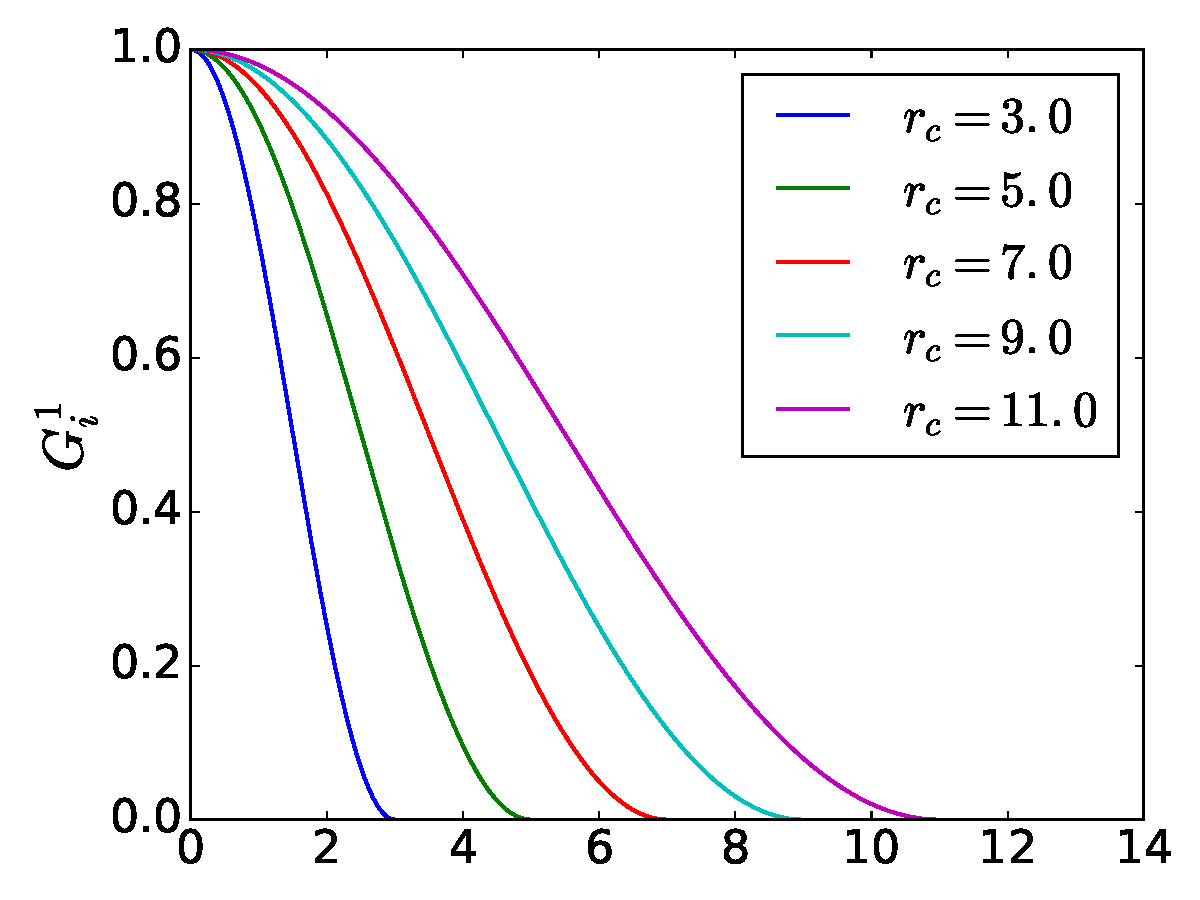
\includegraphics[width=\linewidth]{Figures/Theory/G1.pdf} 
    \label{fig:radialSymmetriFunctions:a} 
    \vspace{1ex}
  \end{subfigure}%% 
  \begin{subfigure}[b]{0.5\linewidth}
    \centering
    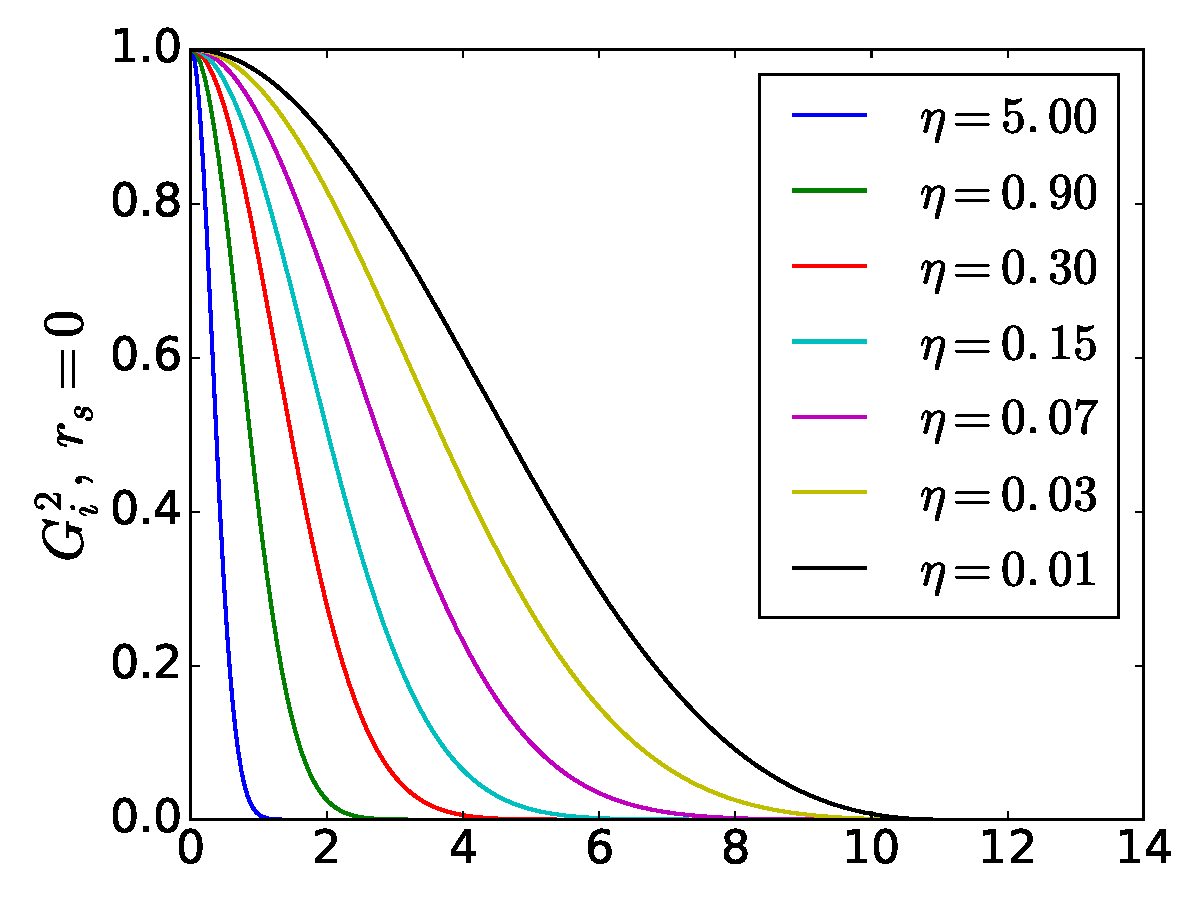
\includegraphics[width=\linewidth]{Figures/Theory/G2_1.pdf} 
    \label{fig:radialSymmetriFunctions:b} 
    \vspace{1ex}
  \end{subfigure} 
  \begin{subfigure}[b]{0.5\linewidth}
    \centering
    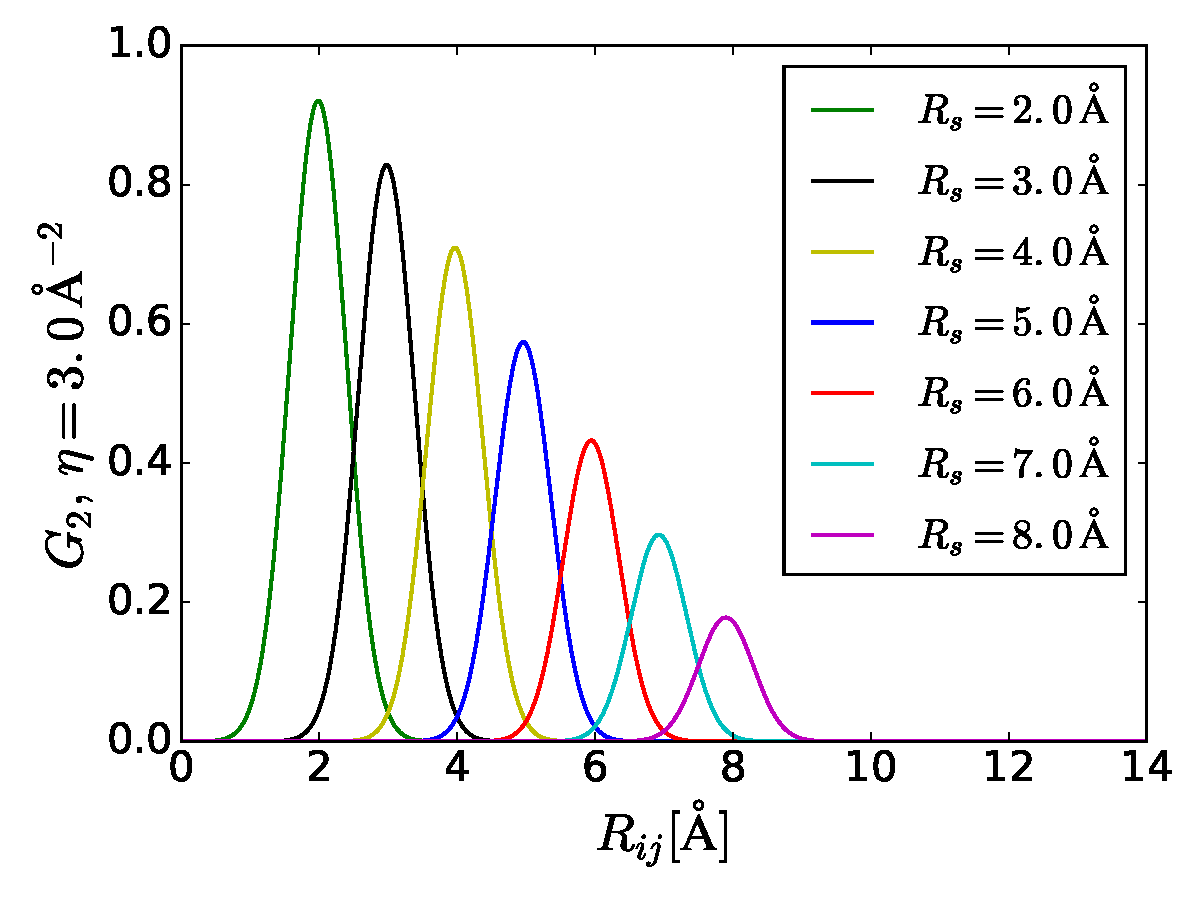
\includegraphics[width=\linewidth]{Figures/Theory/G2_2.pdf} 
    \label{fig:radialSymmetriFunctions:c} 
  \end{subfigure}%%
  \begin{subfigure}[b]{0.5\linewidth}
    \centering
    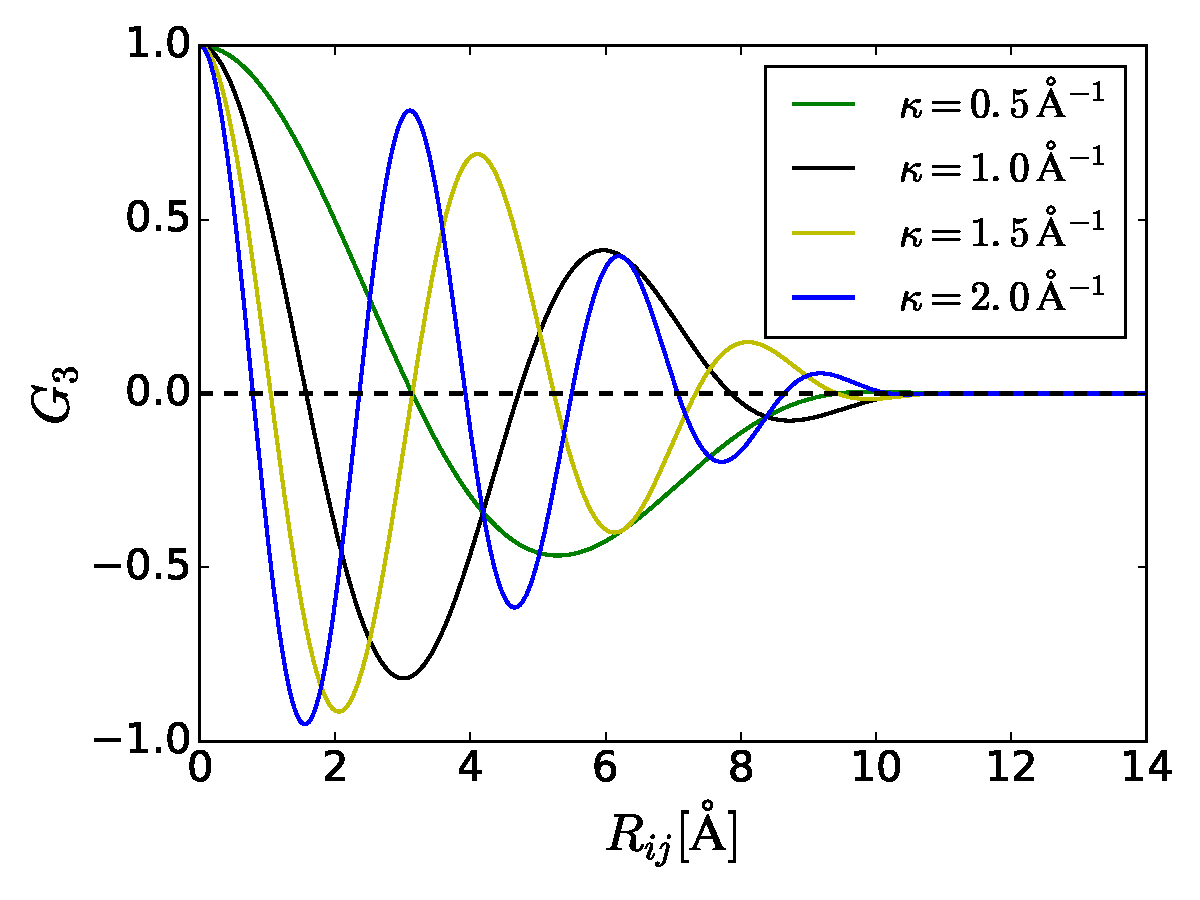
\includegraphics[width=\linewidth]{Figures/Theory/G3.pdf} 
    \label{fig:radialSymmetriFunctions:d} 
  \end{subfigure} 
  \caption{Radial symmetry functions $G^1$, $G^2$ and $G^3$ for an atom with one neighbour only. A set of such 
	   functions represents the radial distrubution of neighbours around a central atom placed at the origin.
	   For $G^2$ and $G^3$ a cutoff $R_c = \SI{11.0}{\angstrom}$ has been used.}
  \label{fig:radialSymmetriFunctions} 
\end{figure}

\subsubsection{Angular symmetry functions}
To obtain a suitable structural fingerprint of the atomic environments, we also need the angular distribution
of neighbouring atoms. This can be achieved by using functions depending on $\theta_{ijk}$, which
is the angle formed by the central atom $i$ and the two interatomic distances $R_{ij}$ and $R_{ik}$. 
The potential is periodic with respect to this angle, so we can use the cosine of $\theta_{ijk}$ instead. 
We thus define an angular symmetry function as a sum over all cosines with respect to any possible triplet
($i$, $j$, $i$), multiplied by Gaussians of the three interatomic distances and the respective cutoff functions,
\begin{equation}
\begin{aligned}
 G_i^4 = 2^{1-\zeta}\sum_{j\neq i}\sum_{k>j} &\bigr[(1 + \lambda \cos\theta_{ijk})^\zeta \cdot
 \exp(-\eta (R_{ij}^2 + R_{ik}^2 + R_{jk}^2)) \cdot \\
 &f_c(R_{ij}) f_c(R_{ik}) f_c (R_{jk})\bigr]
 \label{G4}
\end{aligned}
\end{equation}
This function is zeroed out if any of the interatomic distances is larger than $R_c$. The parameter $\eta$ takes here
into account that the angular contribution depends on the atomic seperations. The angular arrangement can be 
investigated by using different values for $\zeta$ while the normalization factor $2^{1-\zeta}$ ensures that the range of 
values is independent of the choice of $\zeta$. The parameter $\lambda \in {-1,1}$ can be used to invert the shape of the 
cosine function: for $\lambda = +1$ the maxima of the cosine terms are at $\theta_{ijk} = 0^\circ$, 
while for $\lambda=-1$ they are located at $\theta_{ijk} = 180^\circ$. The presence of the cutoff function $R_{jk}$
ensures that only triplets where all three inter-atomic distances are within the cutoff radius are included. 
Another function can be defined that has no constraint on $R_{jk}$,
\begin{equation}
\begin{aligned}
  G_i^5 = 2^{1-\zeta}\sum_{j\neq i}\sum_{k>j} &[(1 + \lambda \cos\theta_{ijk})^\zeta \cdot
 \exp(-\eta (R_{ij}^2 + R_{ik}^2)) \cdot \\
 &f_c(R_{ij}) f_c(R_{ik})]
 \label{G5}
\end{aligned}
\end{equation}
which will generally lead to larger function values than \eqref{G4} because the lack of constraint on $R_{jk}$ results in 
a larger number of non-zero terms in the summation. The angular parts of $G^4$ and $G^5$ are identical, shown in 
\autoref{fig:angularSymmetryFunctions} for different values of $\zeta$. 
\begin{figure}[h]
  \begin{subfigure}[b]{0.5\linewidth}
    \centering
    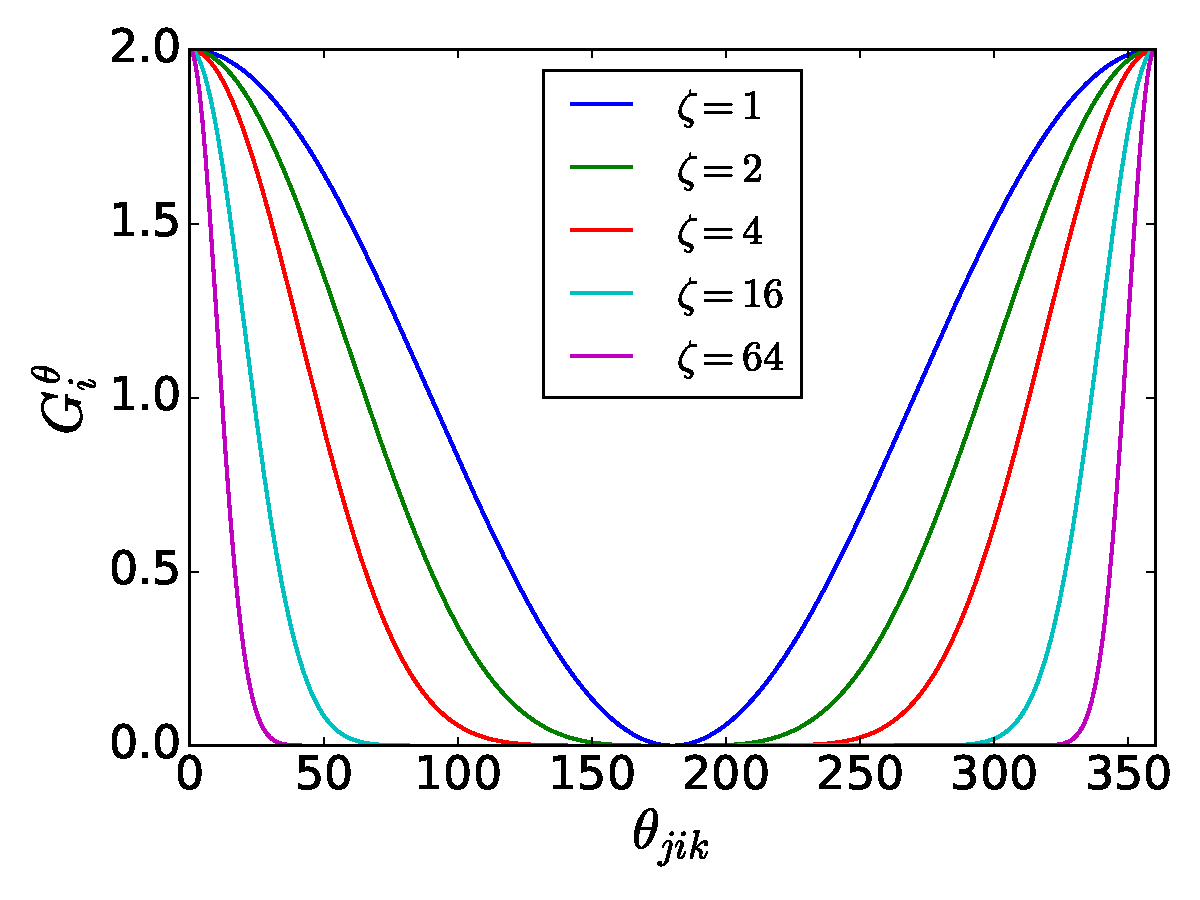
\includegraphics[width=\linewidth]{Figures/Theory/G4G5angular1.pdf}
    \subcaption{}
    \label{fig:angularSymmetryFunctions:a} 
  \end{subfigure}%% 
  \begin{subfigure}[b]{0.5\linewidth}
    \centering
    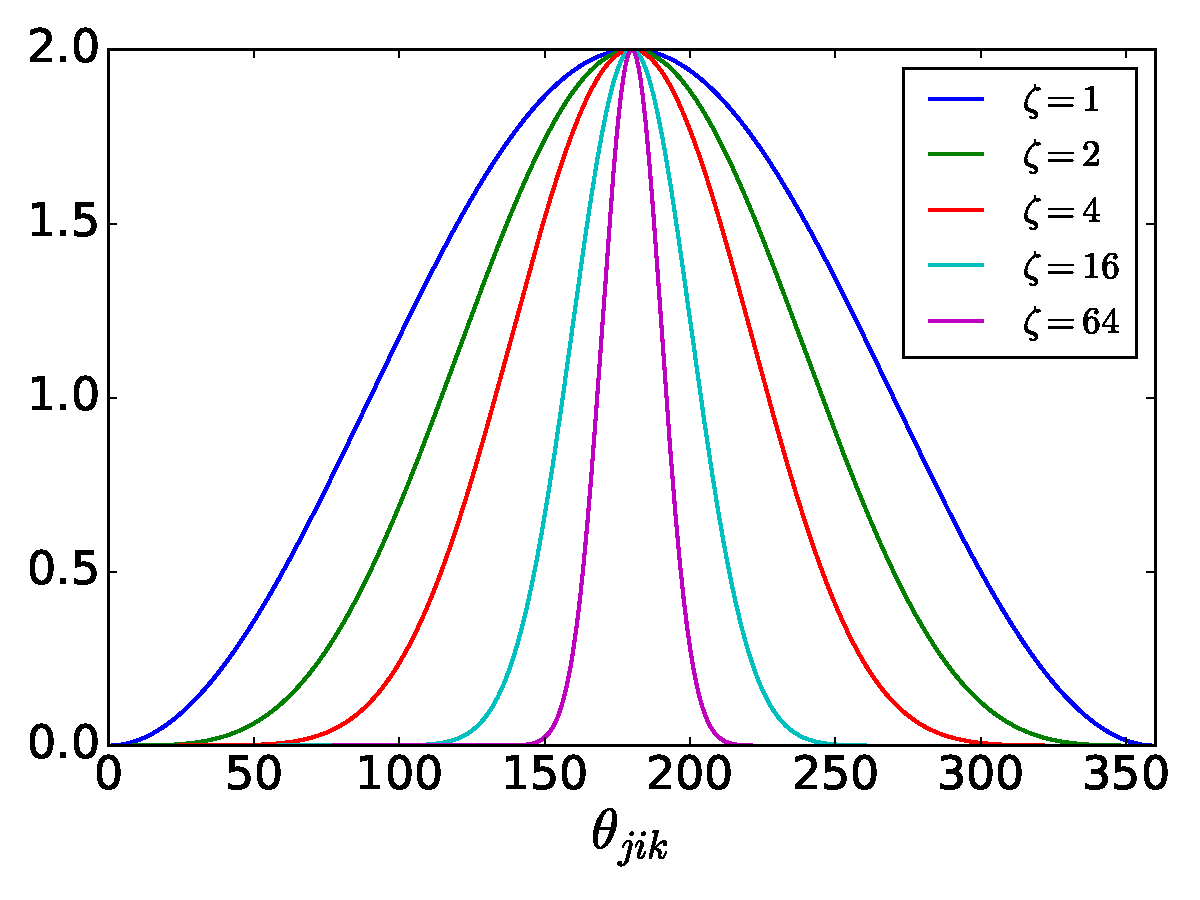
\includegraphics[width=\linewidth]{Figures/Theory/G4G5angular2.pdf} 
    \subcaption{}
    \label{fig:angularSymmetryFunctions:b} 
  \end{subfigure} 
  \caption{Angular part of symmetry functions $G^4$ and $G^5$ for an atom with one neighbour only. A set of such 
	   functions represents the angular distrubution of neighbours around a central atom placed at the origin.
	   $\lambda = +1$ for \autoref{fig:angularSymmetryFunctions:a}, $\lambda=-1$ for \autoref{fig:angularSymmetryFunctions:b}.}
 \label{fig:angularSymmetryFunctions} 
\end{figure}
The parameter values $R_c, \eta, R_s, \zeta$ and $\lambda$ are not automatically optimized, like the weights. 
Once a set of symmetry functions has been determined, they remain fixed during the training of the NN. They are therefore
an integral part of the NN, and need to be evaluated together with the NN itself when applied in simulations. 
The symmetry function set have to be customized for different systems, and different strategies regarding this
is described in \autoref{sec:constructingSymmetry}. A minimum requirement is
to use at least as many symmetry functions as there are degrees of freedom
If this is not the case, the NN recieves insufficient information and will not be able to fit the data properly. 


\subsection{Symmetry functions and forces} \label{sec:symmAndForces}
To integrate Newton's laws in MD simulations we need the forces on all the atoms. The force field associated with a PES
was introduced in section \ref{sec:potentialEnergySurfaces} and is restated here for reference:
\begin{equation}
 \vec{F} = -\nabla E
 \label{forcePES2}
\end{equation}
In the present case, the total energy $E$ of the system is defined as a sum over all the atomic energies \eqref{systemEnergy}. 
Further, we have applied a cutoff so that each atom only gets energy contributions from its atomic environment up 
to a certain distance $R_c$.
The force component $F_{k,\alpha}$, $\alpha = (x,y,z)$ acting on atom $k$ with respect to coordinate $R_{k,\alpha}$,
can therefore be written \cite{Behler11symmetry}
\begin{equation}
 F_{k,\alpha} = -\frac{\partial E}{\partial R_{k,\alpha}} = -\sum_{i=1}^N\frac{\partial E_i}{\partial R_{k,\alpha}}
 = -\sum_{i=1}^{N_k+1}\frac{\partial E_i}{\partial R_{k,\alpha}}
 \label{forceAtomk}
\end{equation}
$N$ is as before the total number of atoms, while $N_k$ is the number of neighbours of atom $k$. 
Note that $E_k$ is included in the above sum - atom $k$ itself contributes to the total energy of its atomic
environment. We therefore have $N_k+1$ contributions. 

NNs have as we have seen well-defined functional forms, and analytical derivatives are therefore readily available.
However, when symmetry transformations is applied, there is only an indirect relation between the energy and the cartesian coordinates
of the atoms. To calculate the force \eqref{forceAtomk} we therefore need to apply the chain rule,
\begin{equation}
 F_{k,\alpha} = -\sum_{i=1}^{N_k+1}\frac{\partial E_i}{\partial R_{k,\alpha}} = 
 -\sum_{i=1}^{N_k+1}\sum_{s=1}^{M_i}\frac{\partial E_i}{\partial G_{i,s}}\frac{\partial G_{i,s}}{\partial R_{k,\alpha}}
 \label{forceAtomkChainRule}
\end{equation}
where $M_i$ is the number of symmetry functions of atom $i$. In other words, we need to sum over all the symmetry functions
of all the neighbours $i$ of atom $k$ and $k$ itself. This is the reverse process of \eqref{BPatomicEnergy},
\begin{equation}
 E_i \rightarrow F_\mathrm{e}[\vec{G}_\mathrm{e}(\vec{R}_{ij})] \rightarrow
 \vec{G}_\mathrm{e}(\vec{R}_{ij}) \rightarrow  \vec{R}_{ij}   
 \label{BPatomicForce}
\end{equation}
where the differentiation is perfomed in the direction of the arrows. 
We realize that the first term
$\partial E_i\partial G_{i,s}$ is the derivative of the output of the atomic NN of atom $i$ with respect to the inputs,
i.e. the gradient of the NN. This is an analytical gradient
which is given by the architecture of the NN, including the values of the weights and biases.
We recall from \ref{sec:backprop} that the backpropagation algorithm calculates the derivatives of all neurons in a NN to obtain
the amount of which each weight and bias should be adjusted during training. We can thus use a slightly modified version
of this algorithm to compute the gradient of a NN,
\begin{enumerate}
 \item Instead of backpropagating the derivative of the cost function, 
 we backpropagate the derivative of the output neuron itself.
 For output neurons with the identity activation function \eqref{outputActivation}, 
 this derivative is 1. 
 \item The derivative is propagated all the way back to the input nodes. During training, the propagation
 stops at the weights connecting the input layer and the first hidden layer. 
\end{enumerate}
This procedure clarifies how a fully-connected feed-forward NN is built: To get the derivative of the output neuron
w.r.t. the input neurons, we have to also compute the derivative of all the neurons in-between because
all nodes in each layer are connected to all nodes in the following layer. 

The second term $\partial G_{i,s}/\partial R_{k,\alpha}$ in \eqref{forceAtomkChainRule} is given by the 
definition of the employed symmetry functions. 
The derivatives of the Behler symmetry functions given in \autoref{sec:symmetryFunctions} are listed in \autoref{app:appendixA1}.

\subsubsection{Change of coordinates}
In a MD simulation we only work with relative or inter-atomic coordinates and potentials. 
The training of neural networks is also based on an atom-centered approach; the cartesian coordinates
that is given as input to the symmetry functions are always atom-centered. This means that the atom
in question is placed at the origin and the positions of all neighbouring atoms are measured relative to 
the origin. Effectively, we are making a change of coordinates to the neighbours $\{j\}$ of the central atom $i$,
\begin{equation}
 \vec{r}_j \rightarrow \vec{r}_j - \vec{r}_i
 \label{changeOfCoordinates}
\end{equation}
This is in accordance with the Behler symmetry functions, which only operate with relative coordinates. 
It is however not trivial how this affects the above equations for the forces, which are not written in 
an atom-centered way. The process of obtaining the forces can be illustrated with an example system
consisting of three atoms of the same element with positions $\vec{r}_i$ where $i = 0,1,2$, shown in \autoref{fig:threeAtoms}.
\begin{figure}[h]
\begin{center}
  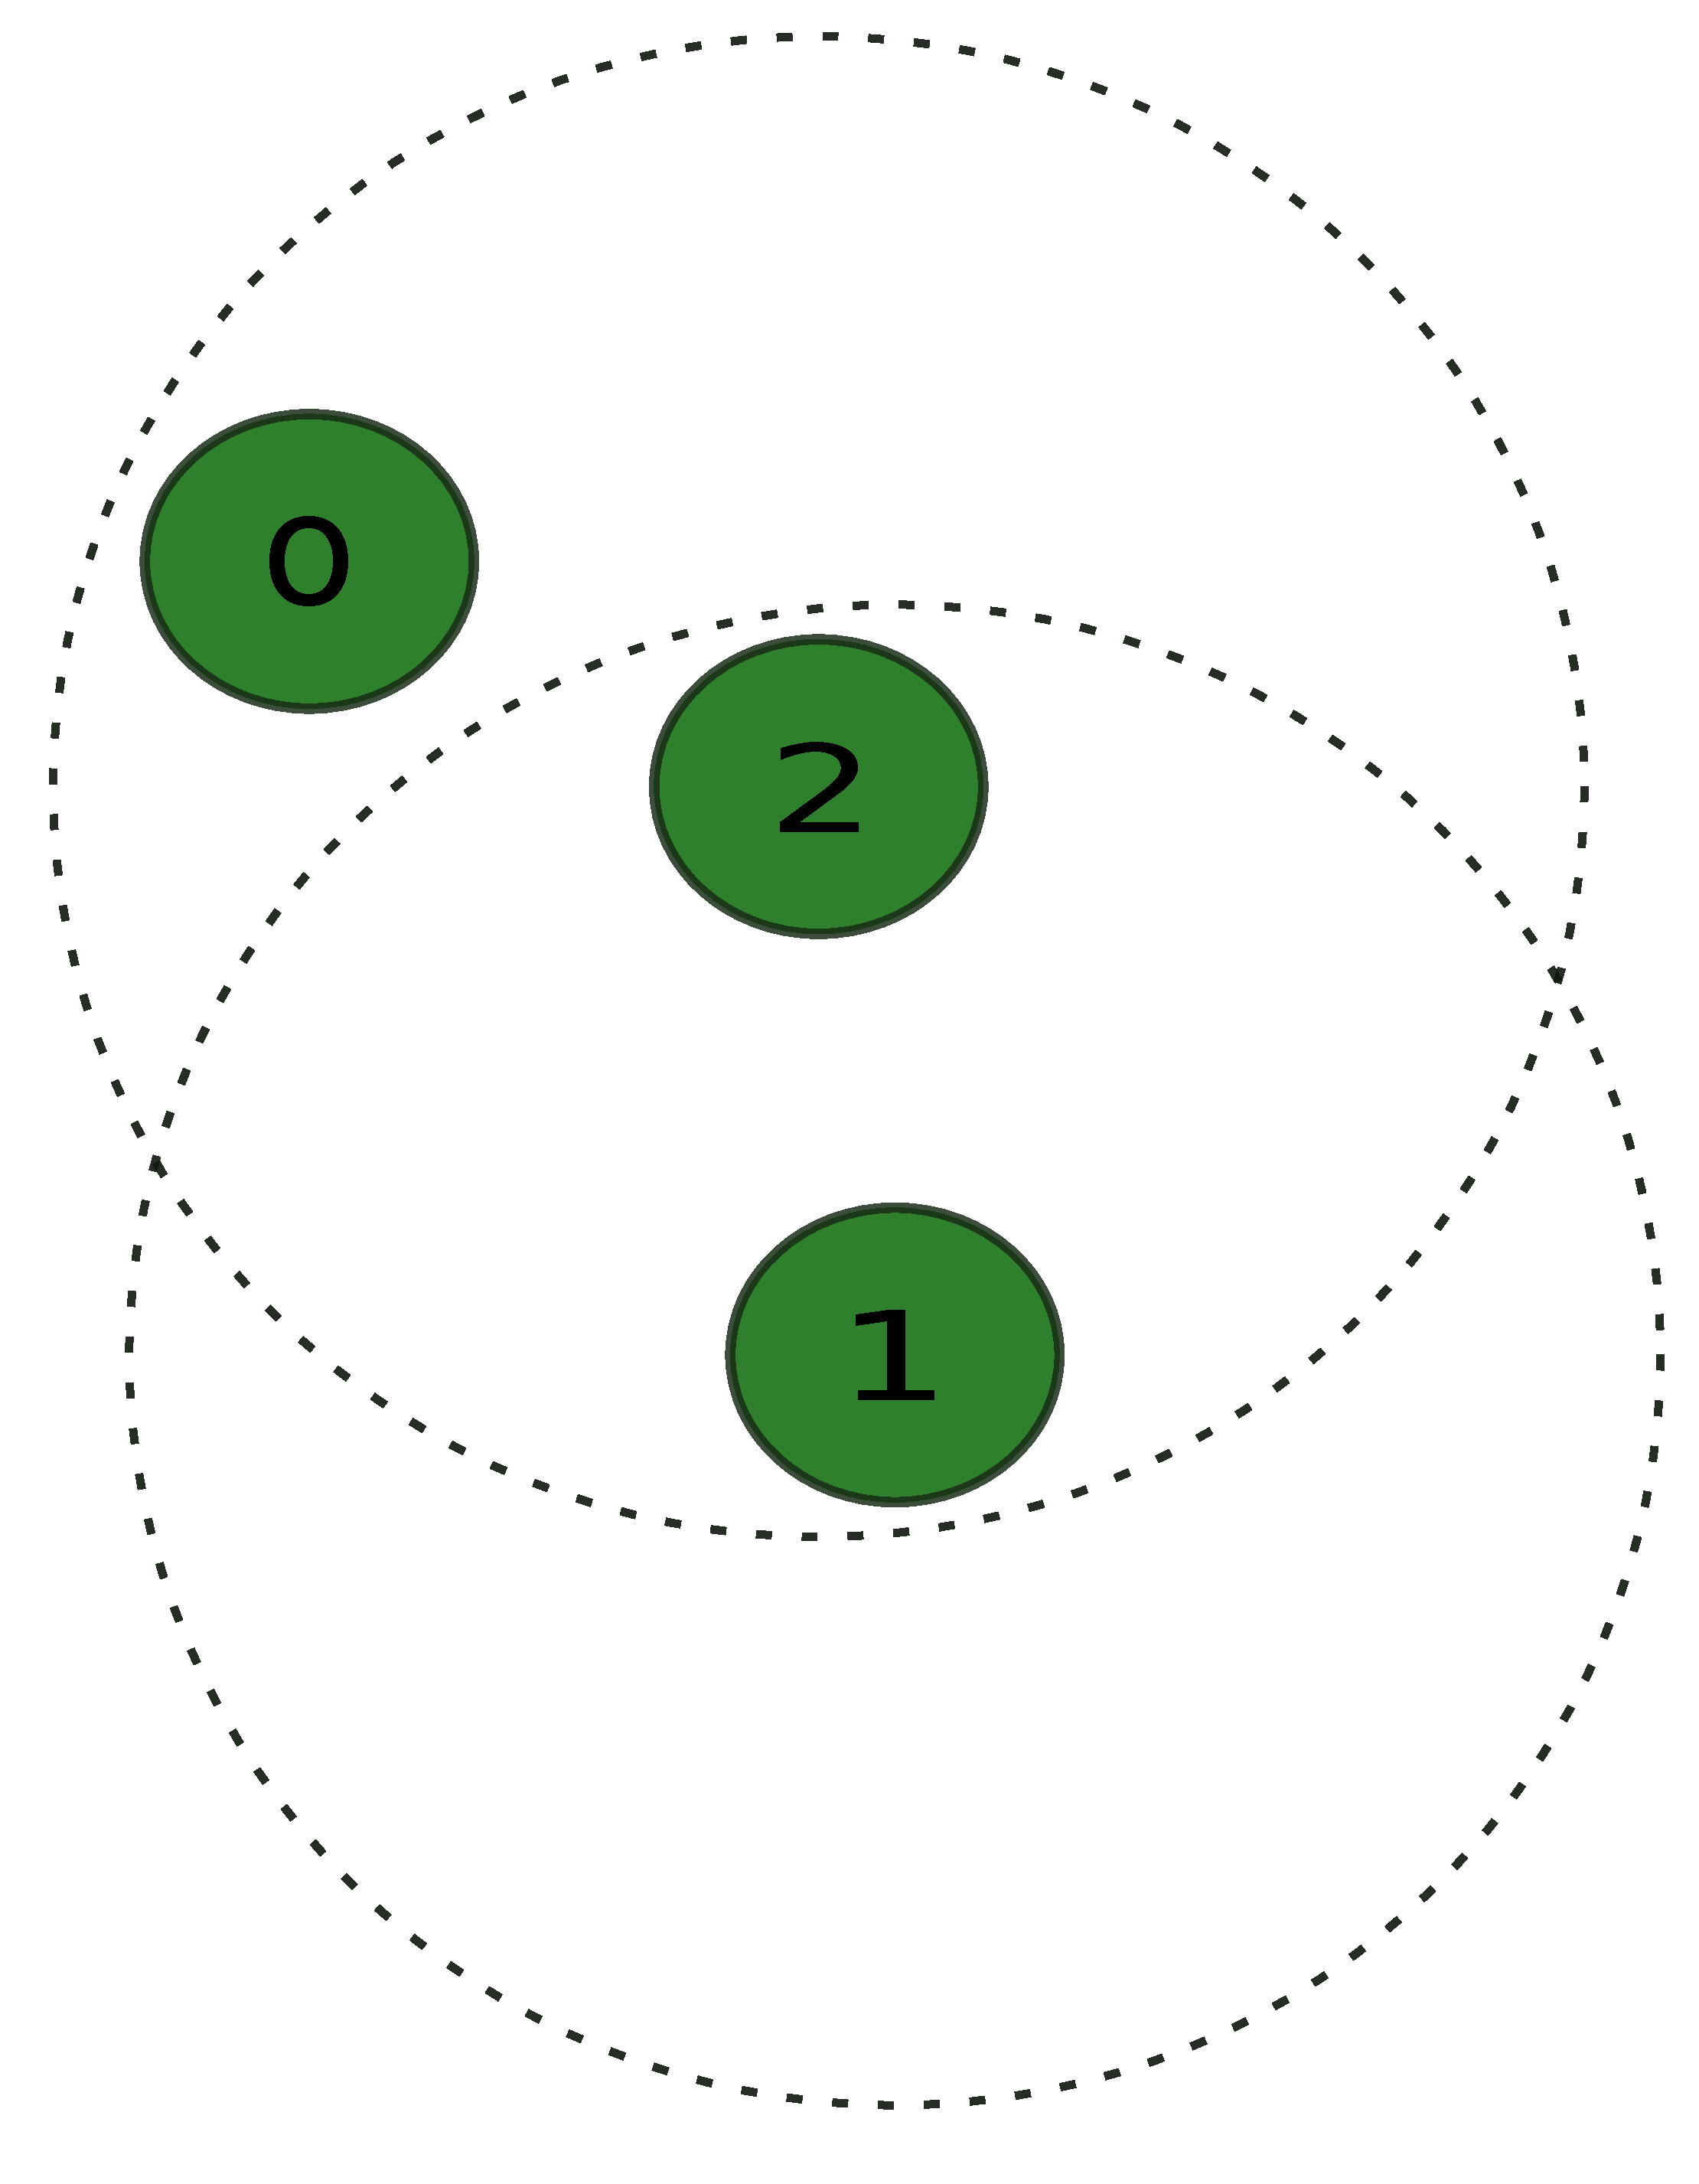
\includegraphics[width = 0.4\linewidth]{Figures/Implementation/3atoms.pdf}
  \caption{Example system of three atoms of the same type. Only atom 2 is inside the cutoff sphere of atom 1, thus we only need to 
	   take the energy of atom 1 and 2 into account to find the force on atom 1. Since the atoms are of the same type,
	   they have identical atomic NNs and symmetry function sets.}
  \label{fig:threeAtoms}
  \end{center}
\end{figure}
We want to find the force on atom 1 in the $x$-direction. Atom 0 is outside the cutoff sphere of atom 1, 
so according to \eqref{forceAtomk} the force is,
\begin{equation}
 F_{1,x} = \frac{\partial E_1}{\partial x_1} + \frac{\partial E_2}{\partial x_1}
 \label{forceOnAtom1}
\end{equation}
For simplicity, we assume that each atom only have two different symmetry functions describing their atomic environment;
one $G_{i,0}^2$ function describing the radial arrangement of neighbours and one $G_{i,1}^5$ dealing with the angular distribution.
Each atomic NN thus have two inputs and one output. 
Since the three atoms are all of the same type, they will have identical NNs $F$ and symmetry vectors. We will therefore 
denote the the two symmetry functions simply as $G^2$ and $G^5$. In the following we apply the notation
$r_{ij} = |\vec{r}_j - \vec{r}_i|$. 
The expressions for $E_1$ and $E_2$ are,
\begin{equation}
 E_1 = F\bigr[G^2(r_{12}) + G^5(r_{12},0,0)\bigr] = F\bigr[G^2(r_{12})\bigr]
 \label{energyAtom1}
\end{equation}
$G^4$ is zero because atom 1 only has one neighbour. Further, 
\begin{equation}
 E_2 = F\bigr[G^2(r_{20}, r_{21}) + G^5(r_{20},r_{21},\theta_{021})\bigr]
 \label{energyAtom2}
\end{equation}
We note that atom 2 receives an energy contribution from both atom 0 and 1, so that 
its $G^2$ function is a sum containing two terms. 
To compute the derivatives of these energies with respect to the $x$-coordinate of atom 1, we
must take into account the change of coordinates \eqref{changeOfCoordinates}. We have that
\begin{equation}
 \frac{\partial G^2(x_{ij})}{\partial x_j} = \frac{\partial G^2(x_{ij})}{\partial x_{ij}}\frac{\partial x_{ij}}{\partial x_j}
 = \frac{\partial G^2(x_{ij})}{\partial x_{ij}}\frac{\partial (x_j-x_i)}{\partial x_j} = 
 \frac{\partial G^2(x_{ij})}{\partial x_{ij}}
 \label{changeOfCoordsSymmetry1}
\end{equation}
and
\begin{equation}
 \frac{\partial G^2(x_{ij})}{\partial x_i} = \frac{\partial G^2(x_{ij})}{\partial x_{ij}}\frac{\partial (x_j-x_i)}{\partial x_i} =
 -\frac{\partial G^2(x_{ij})}{\partial x_{ij}}
 \label{changeOfCoordsSymmetry2}
\end{equation}
which is also valid for the other radial symmetry functions $G^1$ and $G^3$.   
This symmetry, which is a manifestation of Newton's third law,
enable us to calculate the derivatives in \eqref{forceOnAtom1}. For radial symmetry functions
dependent on several atom pairs, \eqref{changeOfCoordsSymmetry1} and \eqref{changeOfCoordsSymmetry2} 
apply to each term in the sum seperately. Further, the symmetry is also present for each atom in a triplet,
\begin{equation}
 \frac{\partial G^5(x_{ij}, x_{ik}, \theta_{jik})}{\partial x_i} = 
 -\frac{\partial G^5(x_{ij}, x_{ik}, \theta_{jik})}{\partial x_{ij}} - 
 \frac{\partial G^5(x_{ij}, x_{ik}, \theta_{jik})}{\partial x_{ik}}
\end{equation}
and 
\begin{subequations}
\begin{align}
 \frac{\partial G^n(x_{ij}, x_{ik})}{\partial x_j} &= \frac{\partial G^n(x_{ij}, x_{ik})}{\partial x_{ij}} \\
 \frac{\partial G^n(x_{ij}, x_{ik})}{\partial x_k} &= \frac{\partial G^n(x_{ij}, x_{ik})}{\partial x_{ik}}
\end{align}
\end{subequations}
i.e. the derivative w.r.t. $i$ is the negative sum of the derivatives w.r.t. $j$ and $k$. This is a symmetry we
have exploited in our code, see \autoref{sec:extendingLammps}. 

To obtain the derivatives of the energies \eqref{energyAtom1} and \eqref{energyAtom2}, we apply the chain rule
\begin{equation}
 \frac{\partial E_1}{\partial x_1} = \frac{\partial F}{\partial G^2(r_{12})}
 \frac{\partial G^2(r_{12})}{\partial x_1} = 
 -\frac{\partial F}{\partial G^2(r_{12})}\frac{\partial G^2(r_{12})}{\partial x_{12}}
\end{equation}
where we have applied the above change of coordinates \eqref{changeOfCoordsSymmetry2}.
Using \eqref{changeOfCoordsSymmetry1}, the derivative of $E_2$ can be calculated correspondingly,
\begin{subequations}
\begin{align}
 \frac{\partial E_2}{\partial x_1} &= 
 \frac{\partial F}{\partial G^2(r_{20}, r_{21})}\frac{\partial G^2(r_{20}, r_{21})}{\partial x_1} + 
 \frac{\partial F}{\partial G^4(r_{20},r_{21},\theta_{021})}\frac{G^4(r_{20},r_{21},\theta_{021})}{\partial x_1} \\
 &= \frac{\partial F}{\partial G^2(r_{21})}\frac{\partial G^2(r_{21})}{\partial x_{21}} + 
 \frac{\partial F}{\partial G^4(r_{20},r_{21},\theta_{021})}\frac{G^4(r_{20},r_{21},\theta_{021})}{\partial x_{21}}
\end{align}
\end{subequations} 
From the definition of $G^2$ \eqref{G2} we see that the sum contains two terms
in the case of atom 2, one for each pair interaction between atom 2 and its two neighbours. 
The interaction term between atom 0 and 2
cancels when differentiated with respect to the coordinates of atom 1, and is thus not included in the force on atom 1. 
 
The sum in $G^4$ \eqref{G4} however, consists of only one term corresponding to the only unique triplet with atom 2
as the central atom. This term is directly dependent on the coordinates of atom 0, which means that 
an atom which is outside the cutoff sphere of atom 1 still contributes to the force. This is an artefact of many-body potentials
like the NNPs employed in this thesis: The force acting on an atom $i$ depends on the positions of the atoms as 
far as $2R_c$ away because \textit{neighbours of neighbours} are included in the
energies that are differentiated to obtain the force. 
This large effective range of atomic interactions is however not of great importance, taking into account
that the interaction strength falls rapidly with distance for most systems where Coulomb forces are not included. 


\subsection{Summary}
In this chapter we have introduced the Behler-Parinello method for constructing NNPs to be used in MD simulations. 
This scheme employs certain symmetry functions that have the following desirable properties,
\begin{enumerate}
 \item They are atom-centered and have an inherent cutoff $R_c$ that defines a chemical environment of tractable size. 
 \item They yield the same number of outputs independent of the number of inputs. 
 \item The order of the inputs is irrelevant. 
 \item They are invariant with respect to translation and rotation.
 \item They have analytic derivatives.
\end{enumerate}
1. and 2. solves the technical issues of the limited and fixed dimensionality of MLPs respectively.
3. and 4. deals with physical symmetries, namely that the energy of an atomic system does not change
if two identical atoms are exhanged, or if the system undergoes a translation or a rotation. 
5. is a wanted property because the symmetry functions are differentiated to obtain forces. 

In \autoref{sec:constructingNNP} we present the complete workflow for constructing a NNP, 
including a description of how to assemble a symmetry function set, found in 
\autoref{sec:constructingSymmetry}.






\part{Implementation and validation}

\chapter{LAMMPS} \label{sec:lammps}
REFERENCE TO MANUAL - FOOTNOTE OF REFERNCE?
LAMMPS (Large-scale Atomic/Molecular Massively Parallel Simulator)
is a classical molecular dynamics simulation package 
developed at Sandia National Laboratories \cite{Plimpton95}. It is written
in highly portable and extendable objected-oriented \texttt{C++}. 
The package's functionality encompasses a wide variety of 
potentials, atom types, integrators, thermostats and 
ensembles and are able to simulate a large number
of different systems, including atoms, molecules, 
coarse-grained particles, polymers, graunular materials
and metals. LAMMPS can be run on a single processor
or in parallell. 

There exist several other molecular dynamics packages, 
like GROMACS, OpenMD, Aber and NAMD that could also
have served the purpose of this thesis. We have chosen
to work with LAMMPS because it is well documented, 
\footnote{\href{http://lammps.sandia.gov/doc/Manual.html}{http://lammps.sandia.gov/doc/Manual.html}}
easy to expand upon \footnote{\href{http://lammps.sandia.gov/doc/Developer.pdf}{http://lammps.sandia.gov/doc/Developer.pdf}}
and because the Computational
physics group at UiO has a lot of experience with using
it for molecular dynamics simulations. 
In this section we will outline the basic usage of LAMMPS, including
a walkthrough of an example input script. We also describe its
class hierarchy and how we can add our own functionality
to the package.

\section{Installing LAMMPS}
We have chosen to install LAMMPS by cloning
the Github repository and compile the source
code by running \texttt{make} in the source directory. 
To compile a serial version of the software, we simply run
the command
\begin{lstlisting}[language=bash]
 make serial
\end{lstlisting}
while the corresponding command for the parallel
MPI version is
\begin{lstlisting}[language=bash]
 make mpi
\end{lstlisting}
New updates can be downloaded by setting an
upstream git remote to point to the LAMMPS
GitHub repository and doing a \texttt{git fetch upstream}. 
LAMMPS also have several additional packages that
can be installed. This can be done by running
\begin{lstlisting}[language=bash]
 make yes-<package name>
\end{lstlisting}
e.g. \texttt{manybody} to install many-body potentials
like Stillinger-Weber and Vashishta. 

\section{LAMMPS input script}
LAMMPS is run by providing an input script as 
argument to the excecutable. This input script
is read line by line and has its own syntax. 
A good way to show the basics an input file
is to look at a simple example of a script
to measure diffusion in liquid argon,
\begin{lstlisting}[style=lammps]
# initialization
units 			metal		
dimension 		3
boundary		p p p		
atom_style		atomic		

# create geometry and atoms
lattice 		fcc 1.08506
variable		Nc equal 10
region 			myRegion block 0 ${Nc} 0 ${Nc} 0 ${Nc}
create_box		1 myRegion
create_atoms	1 box

# set mass and initial temperature
mass			1 1.0
variable		temp equal 300
velocity		all create ${temp} 87287 mom yes 

# compute diffusion
compute 		disp all displace/atom

# potential 
pair_style		lj/cut 2.5
pair_coeff		1 1 1.0 1.0 2.5
neighbor		0.5 bin
neigh_modify	every 20 delay 0 check no

# integration
timestep 		0.01
run_style 		verlet
fix 			integration all nve

# output
thermo			50
thermo_style 	custom step temp density press ke pe etotal 
thermo_modify 	norm yes

# run simulation
run				5000
dump 			diff all custom 100 diff*.dat c_disp[4]
run				10000
\end{lstlisting}
We will in the following briefly explain what
processes that are evoked in LAMMPS when the 
above commands are read. We start with the initialization of 
three basic properties of the simulation: units, boundary conditions and particle types.
\begin{lstlisting}[style=lammps]
 units 		metal
\end{lstlisting}
This command defines the units that are used 
in the simulation and the output. LAMMPS have eight
different unit sets. The \texttt{metal} set measures
distance in \AA{}ngstr\o{}m, energy in eV and temperature
in Kelvin. The choice of units depends on the system
that is investigated and the scale we are looking at.
\begin{lstlisting}[style=lammps]
 boundary 	p p p
\end{lstlisting}
We want to measure diffusion in a bulk
Argon liquid, thus we want to have periodic 
boundary conditions in all three dimensions, 
annotated by a \texttt{p}. LAMMPS can also handle stiff \texttt{f}
and adaptive \texttt{s} non-periodic boundaries. Adaptive
means that the position of the face is set so as to
encompass the atoms in that dimension. 
\begin{lstlisting}[style=lammps]
 atom_style atomic
\end{lstlisting}
Different systems need different information
to be stored for each atom. For style \texttt{atomic}, only
the default attributes are associated with each atom, 
namely coordinates, velocities, atom IDs and types. 
This is sufficient for pair-interacting, non-bonded
systems like Argon.

\noindent Next, we create the geometry of the simulation domain.
\begin{lstlisting}[style=lammps]
lattice 	fcc 5.720
\end{lstlisting}
This defines the initial configuration of the atoms. 
Here, a ffc lattice with a lattice constant of
5.720 is used. Other types of lattices based on
cubic or square unit cells are also available. 
\begin{lstlisting}[style=lammps]
variable	Nc equal 10
region 		simBox block 0 ${Nc} 0 ${Nc} 0 ${Nc}
\end{lstlisting}
The system's geometry is defined with the \texttt{region}
command. The \texttt{block} style is simply a 3-dimensional
straight-faced box with a size of $N_c = 10$ unit
cells in each dimension. We have labelled the 
region \texttt{simBox}. 
The number of unit cells
\texttt{N\_c} is defined as a LAMMPS \texttt{variable}. Variables
can be referenced elsewhere in the script by
writing \texttt{\$\{variable\_name\}} to become part of a new input
command like above. LAMMPS enables many styles
of variables to be defined. 
\begin{lstlisting}[style=lammps]
create_box		1 simBox
create_atoms	1 box
\end{lstlisting}
The command \texttt{create\_box} creates a simulation box 
based on the specified region, in our case the 
\texttt{block} region defined above. The argument specifies
the number of atom types that will be used in the
simulation. Next, \texttt{create\_atoms} with the argument
\texttt{box} fills the simulation
domain with atoms of type 1 on the lattice. 
LAMMPS also lets you create a random collection
of atoms or single atoms at specified coordinates.
\begin{lstlisting}[style=lammps]
mass			1 28
variable		temp equal 300
velocity		all create ${temp} 87287 
\end{lstlisting}
We need to assign mass to the atoms. For metal units, 
mass is measured in grams/mole. The atoms are also
given an initial velocity that corresponds to 
the given initial temperature. 
\begin{lstlisting}[style=lammps]
pair_style		lj/cut 2.5
pair_coeff		1 1 1.0 1.0 2.5
\end{lstlisting}
The choice of potential is made with the 
\texttt{pair\_style} command. We want to simulate
interactions using the cutoff Lennard-Jones potential
with a global cutoff of 2.5 Å. The LJ parameters
are set with \texttt{pair\_coeff}, the way this is done
depends on the potential being used. For our
choice of potential the arguments is as follows:
\texttt{atom-type-1 atom-type-2 sigma epsilon cutoff}. 
The parameters and cutoff can thus be set seperately 
for each pair of atom types.
\begin{lstlisting}[style=lammps]
neighbor		0.5 bin
neigh_modify	every 20 check yes
\end{lstlisting}
These commands sets parameters that affect the 
building of neighbor lists. The first argument
to \texttt{neighbor} is the skin size, while the 
second selects what algorithm is used
to build the lists. The \texttt{bin} style creates 
the lists by binning, which in most cases
(including ours) is the fastest method. 
Further, we can control how often the lists
are built with \texttt{neigh\_modify}. The above arguments
specifies that new neighbour lists are built 
every 20 steps, but every step LAMMPS checks
if any atom has moved more than half the skin distance.
If that is the case, new lists are built. 
\begin{lstlisting}[style=lammps]
timestep 		0.01
run_style 		verlet
fix 			integration all nve
\end{lstlisting}
LAMMPS integrates Newtons' equations of motion
with the velocity-Verlet algorithm by defualt. 
This is the integrator of choice for most MD
applications due to its simplicity and 
symplectic nature (REF TO SECTION). The 
rRESPA integrator \cite{Tuckerman92} scheme is also available.
LAMMPS does however not integrate and update
the positions and velocities of the particles
if not explicitly told so. This is done with
a \texttt{fix}, which is any operation that is applied to the 
system during timestepping. The above fix 
tells LAMMPS to integrate all atoms in the system 
so that they follow trajectories consistent with 
the microcanonical ensemble. 
\begin{lstlisting}[style=lammps]
thermo			50
thermo_style 	custom step temp press ke pe etotal 
thermo_modify 	norm yes
\end{lstlisting}
We can control what thermodynamic properties 
to calculate and output with \texttt{thermo\_style}, while 
\texttt{thermo} decides how often they should be computed. 
We want to output the time step, temperature, 
pressure, kinetic energy, potential energy and total
energy. Also, we want to normalize the extensive
quantities (the energies) by the number of atoms. 
\begin{lstlisting}[style=lammps]
 compute 		disp all displace/atom
 dump 			diff all custom 100 diff*.dat c_disp[4]
\end{lstlisting}
To measure diffusion in the 
Argon liquid, we need to calculate the net
displacement of all atoms. This can be done with a 
\texttt{compute}, which defines a computation that is 
performed on a group of atoms, in this case all atoms.
The \texttt{displace/atom} compute calculates the current
displacement of each atom from its original
coordinates, including all effects due to atoms
passing through periodic boundaries.
For the compute to actually be performed, it needs
to be evoked by other LAMMPS commands, like \texttt{dump}, 
which writes a snapshot of atom quantities to one 
or more files every N timesteps. Computes are 
referenced via the following notation \texttt{c\_ID}, where
ID is the ID of the compute. 
\begin{lstlisting}[style=lammps]
run		5000
\end{lstlisting}
Lastly, we run the simulation for 5000 timesteps. 
LAMMPS allowes several run commands to be issued
after one another. This comes in handy if we want
to thermalize the system before measuring diffusion.
This can be achieved by writing the following commands:
\begin{lstlisting}[style=lammps]
 run 	5000
 dump 	diff all custom 100 diff*.dat c_disp[4]
 run 	10000
\end{lstlisting}
When parsing the second run command, LAMMPS will
continue the dynamics while computing eventual
new fixes, computes, dumps etc. defined since
the last run command. 

This section has illuminated some of the basic
funcionality of LAMMPS through several comments
on a simple input script. Now we move on to
how class hierarchy of LAMMPS is structured. 

\section{LAMMPS structure}
LAMMPS is written in \texttt{C++} in an object-oriented
fashion. The class hierarchy is shown schematically
in \autoref{fig:lammpsClasses}. 
The top-level classes (blue)
are visible anywhere in LAMMPS.
Some selected sub-classes (green and yellow) are displayed. We recognize many 
of the input script commands among these sub-classes
classes; a rule of thumb is that every input script
command has a corresponding class and a
corresponding file name in the source directory. 
For instance, we observe that the cutoff Lennard-Jones potential
used in our input script is a subclass of Pair,
and is evoked by the command
\texttt{pair\_style lj/cut} and the source file is named
\texttt{pair\_lj\_cut}. 
\begin{figure}
\begin{center}
 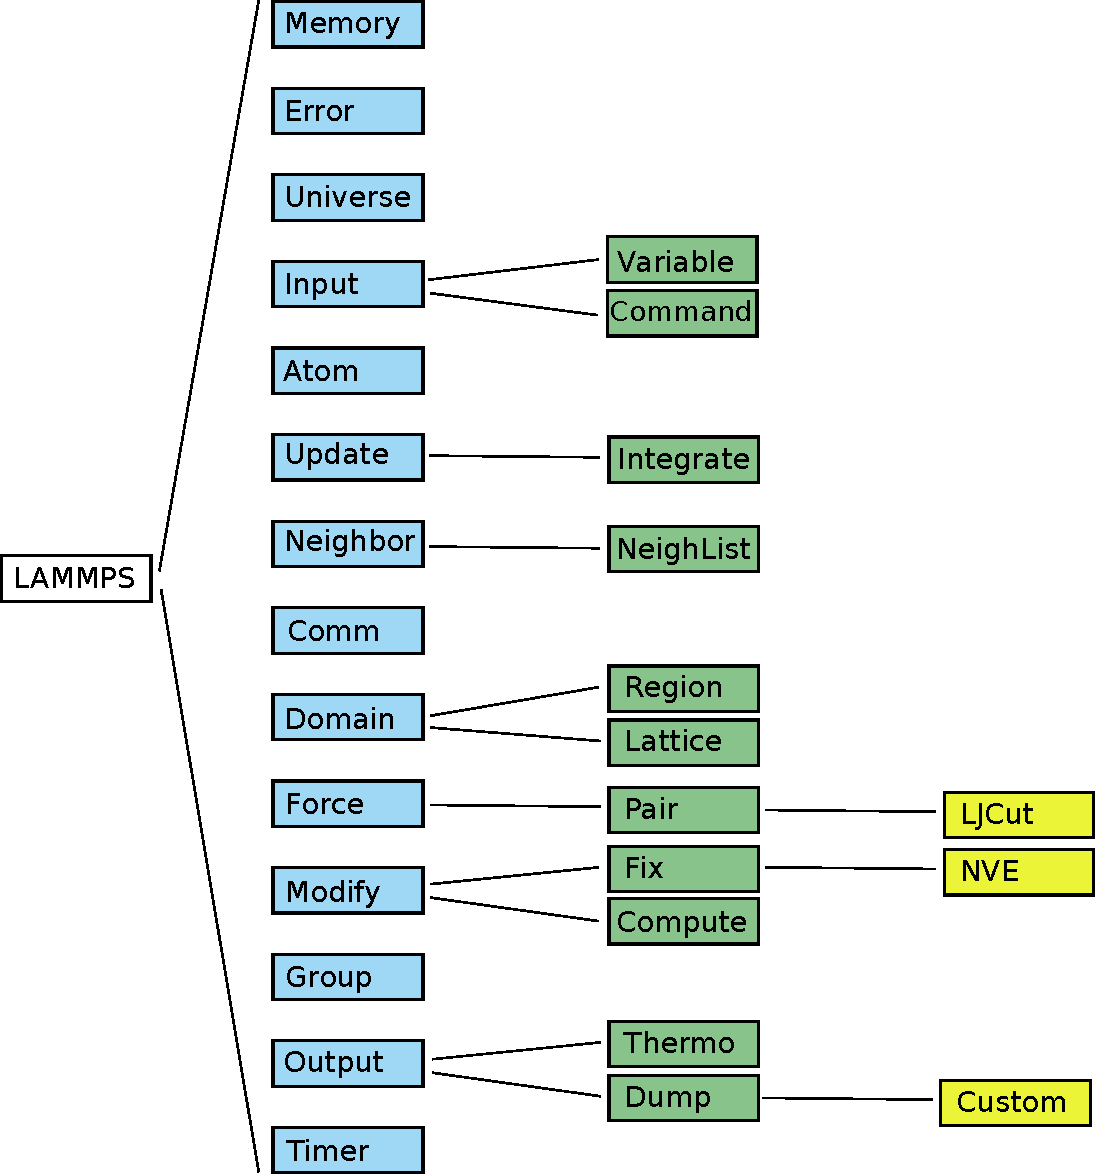
\includegraphics[width = 0.8\linewidth]{Figures/Implementation/lammpsClasses.pdf}
  \caption{Class hierarchy of LAMMPS. The inheritance is from left to right. 
	   The top-level classes (blue) are visible everywhere in the code. Only a selected set 
	   of sub-classes (green and yellow) is displayed, where we recognize many of the input script
	   commands.}
  \label{fig:lammpsClasses}
  \end{center}
\end{figure}

We will not go into detail about the functionality
and communication of these classes. The one
that is the most relevant for this work is the \texttt{Pair} class. 
This is the parent class of non-bonded or pair-wise potentials, which
in LAMMPS includes many-body potentials like Stillinger-Weber and 
Vashishta. The NN potential in this thesis falls 
under this category, and thus inherits from \texttt{Pair}. 
In the following section we will describe how 
LAMMPS can be extended with such a new \texttt{pair\_style}.

\section{Extending LAMMPS} \label{sec:extendingLammps}
To extend LAMMPS with a new component, we 
simply add a new \texttt{*.cpp} and \texttt{*.h} file to the 
source directory and re-compile. The new class
will (in theory) work with all other LAMMPS 
classes without breaking any functionality. 
A good strategy is to start with an existing potential
source file that is somewhat similar to the one 
we want to make, instead of programming from scratch.
We aim to construct a many-body non-bonded potential, and 
have chosen to base our implementation on the 
Stillinger-Weber potential file, \texttt{pair\_sw.cpp}.

The new potential class is added to LAMMPS with the following function call in the header file,
\begin{lstlisting}[language=c++]
 PairStyle(nn/manybody,PairNNManyBody)
\end{lstlisting}
The first argument is the name the potential will have in the input script, while 
the second is the name of the class. 
To use our new NN potential in a simulation we simply write,
\begin{lstlisting}[style=lammps]
 pair_style 	nn/manybody
\end{lstlisting}
in the input script. This command evokes two functions that need to be implemnted: \texttt{settings}
and \texttt{init\_style}. The former controls the number of arguments to 
\texttt{pair\_style}, which in our case is zero, while the latter
decides what kind of neighbour lists that LAMMPS should provide to the potential. Our NN potential needs 
full neighbour lists to be able to compute three-body terms, something which applies to all many-body potentials. 

The parent class \texttt{Pair} has three \textit{pure virtual member functions}, i.e. functions that are required
to be implemented by a derived class: \texttt{compute}, \texttt{coeff} and the aforementioned \texttt{settings}. 
The \texttt{compute} method is where the forces and energies are calculated. This function is called
once each time step by the Verlet algorithm and the resulting forces are used to integrate Newton's equations
of motion. The coefficients of the employed potential are set in \texttt{coeff}, which in the case of a NN potential
is the weights, biases and symmetry function parameters. 
These are read from file, and based on information on the architecture of the NN and 
choice of activation function, the network is reconstructed as a set of Armadillo matrices and 
vectors. This is achieved with the input script command,
\begin{lstlisting}[style=lammps]
 pair_coeff		* * <path-to-saved-NN> <cutoff> 
\end{lstlisting}
where the wildcard asterisks signify that the coefficients span all atom types and are read from file. 
Note that also the symmetry parameters employed during training are read 
If there are more than one element, a seperate NN file is read for each one. 
An example is $\mathrm{SiO}_2$,
\begin{lstlisting}[style=lammps]
 pair_coeff 		* * <path-1> <path-2> Si O <cutoff>
\end{lstlisting}
The process of employing the NN to calculate the forces and energies of all atoms in the system 
is described as follows,
\begin{enumerate}
 \item Access various variables like the vector of atom coordinates and the neighbour lists of each atom.
 \item Loop through all atoms. For each atom $i$:
 \begin{enumerate}
  \item Construct input vector to the NN by evaluating the symmetry functions for all pairs and triplets below the cutoff radius. 
	The coordinates, types, angles etc. of all pairs and triplets must be stored for later force calculations. 
  \item Evaluate the NN corresponding to the element of atom $i$ to obtain its total atomic energy.
  \item Calculate the gradient of the energy w.r.t. the symmetry function values by backpropagation.
  \item Differentiate the symmetry functions w.r.t. to the coordinates of all neighbours to obtain the total force on atom $i$.
 \end{enumerate}
\end{enumerate}
This process determines the structure of the \texttt{nn/manybody} \texttt{compute} function. 
We start out by accessing various variables needed to compute the forces,
\begin{minted}{c++}
double **x = atom->x;      // atom coordinates
double **f = atom->f;      // forces
int *type = atom->type;    // type of each atom	
int nlocal = atom->nlocal; // no. of atoms belonging to current processor  

int inum = list->inum;     // length of list containing all neighbour lists
int *ilist = list->ilist;  // local indicies of all local atoms
int *numneigh = list->numneigh; // lengths of each neighbour list
int **firstneigh = list->firstneigh; // all neighbour lists
\end{minted}
Next, we loop through all atoms in \texttt{ilist}. For each atom, we evaluate 
the two-body and three-body symmetry functions with the symmetry parameters read from file. 
We also store certain information on all neighbours. 
\begin{minted}{c++}
for (int ii = 0; ii < inum; ii++) {
  int i = ilist[ii];
  int itype = map[type[i]];

  double xtmp = x[i][0];
  double ytmp = x[i][1];
  double ztmp = x[i][2];

  // neighbour list of atom i
  int *jlist = firstneigh[i];
  int jnum = numneigh[i];
  
  // collect all pairs
  for (int jj = 0; jj < jnum; jj++) {
    int j = jlist[jj];
    j &= NEIGHMASK;
    tagint jtag = tag[j];
    int jtype = map[type[j]];

    double delxj = x[j][0] - xtmp;
    double delyj = x[j][1] - ytmp;
    double delzj = x[j][2] - ztmp;
    double rsq1 = delxj*delxj + delyj*delyj + delzj*delzj;

    if (rsq1 >= cutoffSquared) continue;   
    double rij = sqrt(rsq1);
    
    // store relative coordinates (delxj, delyj, delzj), distance rij, 
    // index j and type jtype
    
    // apply two-body symmetry...
    
    // collect all triplets
    for (int kk = jj+1; kk < jnum; kk++) {
      // apply three-body symmetry and 
      // store configurations of all triplets...
\end{minted}
We are now ready to evalute the NN with the input vector of symmetry values. 
The NN is implemented as a function, shown here in the monatomic case for brevity,
\begin{minted}{c++}
double PairNNManyBody::network(arma::mat inputVector) {

  // no activation for input layer
  m_preActivations[0] = inputVector;
  m_activations[0] = m_preActivations[0];

  // hidden layers
  for (int i=0; i < nLayers; i++) {
    m_preActivations[i+1] = m_activations[i]*m_weights[i] + m_biases[i];
    m_activations[i+1] = sigmoid(m_preActivations[i+1]);
  }

  // identity activation for output layer
  m_preActivations[nLayers+1] = m_activations[nLayers]*m_weights[nLayers] + 
				m_biases[nLayers];
  m_activations[nLayers+1] = m_preActivations[nLayers+1];

  // return activation of output neuron
  return m_activations[nLayers+1](0,0);
}
\end{minted}
where \texttt{sigmoid(A)} is a function that returns the sigmoid \eqref{sigmoidActivationFunction} 
of each element of a matrix \texttt{A}. 
Each variable with the \texttt{m\_} prefix is an \texttt{std::vector} containing a set of Armadillo matrices. 
For instance, \texttt{m\_weights[0]} is a matrix of all weights connecting the input layer 
and the first hidden layer. This results in highly readable code that is very similar to the mathematical 
description \eqref{forwardPropMatrix}, 
\footnote{The weight-activation multiplication is in reverse order in the code because we use row vectors instead of column vectors.
Also, the indexing of the weight and bias vectors are different than in \eqref{forwardPropMatrixLammpsChapter}, as 
the activation and preactivation vectors also include the input layer. This also applies to the implementation
of backpropagation.}
\begin{equation}
 \begin{aligned}
  \vec{u}_l &= W_l\vec{y}_{l-1} + \vec{b}_l \\
  \vec{y}_l &= f_l(\vec{u}_l)
  \label{forwardPropMatrixLammpsChapter}
\end{aligned}
\end{equation}
The NN is differentiated by employing backpropagation according to the procedure oulined in \autoref{sec:symmAndForces},
\begin{minted}{c++}
arma::mat PairNNManyBody::backPropagation() {

  // derivative of output neuron is 1
  arma::mat output(1,1); output.fill(1);
  m_derivatives[nLayers+1] = output;

  // we can thus compute the error vectors for the other layers
  for (int i=nLayers; i > 0; i--) {
      m_derivatives[i] = 
	  ( m_derivatives[i+1]*m_weightsTransposed[i] ) %
          sigmoidDerivative(m_preActivations[i]);
  }

  // no activation function for input layer
  m_derivatives[0] = m_derivatives[1] * m_weightsTransposed[0];

  return m_derivatives[0];
\end{minted}
and we compare to \eqref{backPropMatrix},
\begin{equation}
 \vec{\delta}_l = \vec{y}^\prime_l \odot (W^T_{l+1}\vec{\delta}_{l+1}) \cdot 
 \label{backPropMatrixLammpsChapter}
\end{equation}
Consequentially, the output and gradient of the NN is obtained simply by the two function calls,
\begin{minted}{c++}
evdwl = network(inputVector);
arma::mat dEdG = backPropagation();
\end{minted}
We remember from \autoref{sec:symmAndForces} that the force is the product of the gradient of the NN and 
the symmetry functions \eqref{forceAtomkChainRule},
\begin{equation}
 F_{i,\alpha} = -\sum_{j=1}^{N_i+1}\frac{\partial E_j}{\partial R_{i,\alpha}} = 
 -\sum_{j=1}^{N_j+1}\sum_{s=1}^{M_j}\frac{\partial E_j}{\partial G_{j,s}}\frac{\partial G_{j,s}}{\partial R_{i,\alpha}}
 \label{forceAtomkChainRuleLammpsChapter}
\end{equation}
Here the NN potential differs from ordinary many-body potentials, which 
compute forces from each neighbour on-the-fly: The potential energy of atom $i$
can only be calculated w.r.t all neighbours \textit{simultaneously}. We therefore have to loop over the neighbours once more
to calculate the forces, which is why we store the configurations of all pairs and triplets below the cutoff; to 
avoid recalculations. We show an excerpt of the code that implements \eqref{forceAtomkChainRuleLammpsChapter},
\begin{minted}{c++}
for (int s=0; s < m_numberOfSymmFunc; s++) {

  // G2
  if ( m_parameters[s].size() == 3 ) {
    arma::mat dG2(1,neighbours);

    // calculate cerivative of G2 for all pairs
    dG2dR(Rij, m_parameters[s][0],
	  m_parameters[s][1], m_parameters[s][2], dG2);

    // chain rule: all pair forces
    arma::mat fpairs = -dEdG(0,s) * dG2 / Rij;

    // loop through all pairs
    for (int l=0; l < neighbours; l++) {
      double fpair = fpairs(0,l);

      // force on atom i
      fx2 -= fpair*drij(0,l);
      fy2 -= fpair*drij(1,l);
      fz2 -= fpair*drij(2,l);

      // N3L: force on neighbour
      f[tagsj[l]][0] += fpair*drij(0,l);
      f[tagsj[l]][1] += fpair*drij(1,l);
      f[tagsj[l]][2] += fpair*drij(2,l);
    }
  }

  // G4/G5
  else {
    for (int l=0; l < neighbours-1; l++) {
      // calculate derivative of G4 or G5 for all triplets (i,j,k)
      // and assign forces to all three atoms
\end{minted}
The vectors \texttt{Rij} and \texttt{drij} contain the distances to and relative coordinates of all 
pairs. Note that we assign each pair force $\vec{F}_{ij}$ both to atom $i$ and neighbour $j$, in accordance with 
Newton's third law. This is a requirement for our implementation 
to work: \eqref{forceAtomkChainRuleLammpsChapter} states that
the force on atom $i$ is the derivative of the energies of all neighbours and $i$ itself. This also applies to all neighbours $j$
of atom $i$: each neighbour experiences a force contribution  $\partial E_i / \partial R_{j,\alpha}$. To avoid 
having to store all atomic energies $E_i$, we therefore take care of this contribution when $E_i$ is available. 
The alternative is to compute and store the energies and the environments of all atoms before calculating the forces, but this
is tedious and requires too much storage for large systems. 





\chapter{TensorFlow}
TensorFlow \cite{Abadi15} \cite{Abadi16} is an open source software library 
developed by Google 
for numerical computation using data flow graphs (DFG). 
A DFG is a graphical representation of how data is
advanced through a system, including what kind of information is input
to and output from the system and where data is stored.
The data flow is represented as a directed graph
with a number of \textit{nodes} that is connected by
\textit{edges}. In TensorFlow, nodes represent
mathematical operations, while the edges represent
the multidimensional data arrays (tensors) 
communicated between them.
\begin{figure}
\centering
  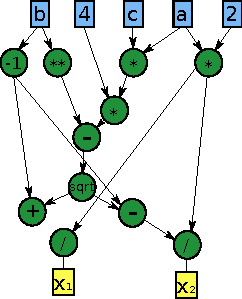
\includegraphics[width=0.4\linewidth]{Figures/Implementation/DFG.pdf}
  \caption{Data flow graph for the solutions \eqref{quadraticEquationSolution} of a 
	   quadratic equation \eqref{quadraticEquation}. The nodes (green circles) are mathematical 
	   operations connected by edges (arrows) that show the data flow direction. Inputs and outputs
	   are marked as rectangular boxes. Reproduced from:
  \href{http://web.cecs.pdx.edu/mperkows/temp/JULY/data-flow-graph.pdf}{http://web.cecs.pdx.edu/mperkows/temp/JULY/data-flow-graph.pdf}} 
  \label{fig:DFG}
\end{figure}

A simple example of a DFG is displayed in \autoref{fig:DFG}, which is a visualization of the flow of data
for the (real) solutions 
\begin{align}
 x_1 &= \frac{-b + \sqrt{b^2 - 4ac}}{2a} \\
 x_2 &= \frac{-b - \sqrt{b^2 - 4ac}}{2a}
 \label{quadraticEquationSolution}
\end{align}
of a quadratic equation
\begin{equation}
 ax^2 + bx + c = 0
 \label{quadraticEquation}
\end{equation}
We observe that each node (green circles)
contain the mathematical operations needed to compute
\eqref{quadraticEquationSolution}, while the arrows
(edges) show what data each node recieve and where
the output is sent. The inputs and outputs
of the graph is marked with rectangular
boxes. 

TensorFlow was originally developed by 
the Google Brain Team \footnote{\href
{https://research.google.com/teams/brain/}{https://research.google.com/teams/brain/}}
with the purpose of conducting machine learning and 
deep neural networks research, but is 
applicable in other domains as well, e.g. for
solving partial differential equations. 
The package incorporates
a wide variety of machine learning algorithms, including
convolutional neural networks and recurrent neural networks.
A computation expressed using TensorFlow can 
be executed on a wide variety of devices and systems, 
from mobile phones to large-scale distributed systems
and GPUs. 

In this chapter we will go through a simple 
example on how to build a computational graph 
with TensorFlow, and how to train a
feed-forward neural network. But first, a few
tips on how to install the software. 

\section{Installing TensorFlow}
The easiest way to install TensorFlow on Ubuntu
\footnote{\href{https://www.tensorflow.org/install/install\_linux}
{https://www.tensorflow.org/install/installlinux}}
is to use pip, \footnote{\href{https://pip.pypa.io/en/stable/}
{https://pip.pypa.io/en/stable/}}
a package management system for software written in 
Python, installed with the command
\begin{lstlisting}[language=bash]
 $ sudo apt-get install python-pip python-dev
\end{lstlisting}
TensorFlow can be installed with or without GPU 
support. The GPU version requires a system with
 CUDA-enabled NVIDIA GPUs
\footnote{\href{https://developer.nvidia.com/cuda-gpus}
{https://developer.nvidia.com/cuda-gpus}}. 
We have used the CPU version for the
development of our code, which is installed
with the command
\begin{lstlisting}[language=bash]
 $ pip install tensorflow
\end{lstlisting}
A simple
\begin{lstlisting}[language=bash]
 $ python -c "import tensorflow"
\end{lstlisting}
will test if the installation was succesful. 

\section{TensorFlow basic usage}
TensorFlow relies on highly-optimized
\texttt{C++} for its computations, but offers
APIs \footnote{\href{https://www.tensorflow.org/api_docs/}
{https://www.tensorflow.org/api\_docs/}}
in both \texttt{Python},
\texttt{C++} and a few other languages. 
The \texttt{Python} API is at present the most
complete, the easiest to use and the best documented.
We have therefore chosen to use \texttt{Python}
to train neural networks. For a discussion
on ways to import a trained NN to \texttt{C++} see
\autoref{sec:extendingLammps}
and \autoref{sec:timeUsage}. 

\subsection{Hello world}
As already mentioned, a TensorFlow computation
is described by a graph which consists of nodes
that communicate with multi-dimensional arrays along
interconnected edges. Each node has zero or more
outputs, and represents the instantation
of an \textit{operation}. Each operation
occurs within a so-called \textit{session}. 
A \texttt{Hello world!} program can be written as
\begin{lstlisting}[language=python]
import tensorflow as tf

hello = tf.constant('Hello world!')
sess = tf.Session()
print sess.run(hello)
# --> Hello world!
\end{lstlisting}
This simple example outlines the general
workflow for building a TensorFlow graph,
\begin{enumerate}
 \item Declare nodes (operations)
 \item Initiate a session
 \item Run operations within session
\end{enumerate}
The only operation in the above example
is the built-in TF constant that holds the 
\texttt{Hello world!} string, and the 
corresponding DFG only consists of one node. 
In more involved examples, visualizing 
the DFG can be useful for finding out how 
the script works. This is done with the 
included TF visualization tool TensorBoard.
We will now look at how to construct a neural network with TF and
visualize the corresponding DFG. 

\subsection{Creating a neural network} \label{sec:TensorFlowCreatingNN}
In \autoref{sec:backprop} we demonstrated that a NN can be constructed 
as a set of matrix-vector multiplications and additions which are input to certain activation functions. 
The equations for evaluting a NN were \eqref{forwardPropMatrix},
\begin{equation}
 \begin{aligned}
  \vec{u}_l &= W_l\vec{y}_{l-1} + \vec{b}_l \\
  \vec{y}_l &= f_l(\vec{u}_l)
  \label{forwardPropMatrix}
 \end{aligned}
\end{equation}
We now want to construct a NN with 3 inputs neurons, one hidden layer with 10 neurons and 1 output neuron. 
We use the sigmoid \eqref{sigmoidActivationFunction} activation function for the hidden layer, while 
the output layer have the identity activation function \eqref{outputActivation}.
This can be achieved with the following \texttt{python} script,
\begin{minted}{python}
import tensorflow as tf

# NN parameters
inputs 	= 3
nodes 	= 10
outputs = 1

# declare input tensor
inputLayer = tf.placeholder( tf.float32, [None,inputs] )

# weights input layer -> hidden layer and biases hidden layer
W1 = tf.Variable( tf.random_normal([inputs,nodes]) )
b1 = tf.Variable( tf.constant(0.1, shape=[nodes]) )

# activation hidden layer
preAct1 = tf.add( tf.matmul(inputLayer, W1), b1 ) 
act1 = tf.nn.sigmoid(preAct1)

# weights hidden layer -> output layer and bias output layer
W2 = tf.Variable( tf.random_normal([nodes,outputs]) )
b2 = tf.Variable( tf.constant(0.1, shape=[outputs]) )

# activation output layer
preActOutput = tf.add( tf.matmul(act1, W2), b2 ) 
activationOutput = preActOutput
\end{minted}
There are several aspects of the TensorFlow \texttt{python} API to comment on here. 
We observe that the input layer is declared as a TF \texttt{placeholder}. This is a special
type of TF tensor that is not initialized with any values, but is rather fed with data on its execution.
Specifying the first component of its shape as \texttt{None} signifies that we can supply an arbitrary 
number of data points at the same time.
These properties enables the same NN to be evaluated for different data vectors of varying size on-the-fly during training, 
explained in more detail below. 

The weights and biases are declared as TF \texttt{Variables}. These are the trainable parameters 
of the computational graph, and are normally constructed as random numbers. In the present case,
the weights are normally distributed numbers while the biases are all set to the same value 0.1. 
We note that the shapes of the weight matrices and bias vectors are in accordance with the description in 
\autoref{sec:MLPmodel}.

The activations (outputs) of each layer are calculated according to \eqref{preActivationLayer} and \eqref{activationLayer}. 
Together with the input \texttt{placeholder}, these are of type \texttt{tf.Tensor}, i.e. nodes in the computational 
graph. 

\subsection{Visualizing the graph}
We can use TensorBoard to visualize the DFG of the above script. The DFG for the present example is quite
simple, but for more involved models it quickly becomes difficult to keep track of all the different components. 
A convenient tool to order and group the DFG is \textit{name scoping}. Both \texttt{Tensors} and \texttt{Variables} can 
be name scoped and TensorBoard uses this information to define a hierarchy of the nodes in the graph. 
An example of name scoping is
\begin{lstlisting}[language=python]
 with tf.name_scope('layer1'):
    W1 = tf.Variable( tf.random_normal([inputs,nodes]), name='weights')
    b1 = tf.Variable( tf.constant(0.1, shape=[nodes]), name='biases')
\end{lstlisting}
which results in the following names,
\begin{itemize}
 \item \texttt{layer1/weights}
 \item \texttt{layer1/biases}
\end{itemize}
Additionally, TensorBoard will group the two variables together under \texttt{layer1}. 
To save the graph to file we have to start a TF session. The following script 
deploys name scoping, initiates a session and writes the DFG to file,
\begin{minted}{python}
import tensorflow as tf

# NN parameters
inputs = 3
nodes = 10
outputs = 1

with tf.name_scope('inputLayer'):
    inputData = tf.placeholder(tf.float32, [None,inputs], name='inputData')

with tf.name_scope('layer1'):
    
    W1 = tf.Variable( tf.random_normal([inputs,nodes]), name='weights' )
    b1 = tf.Variable( tf.constant(0.1, shape=[nodes]), name='biases' )
 
    preAct1 = tf.add( tf.matmul(inputData, W1), b1, name='preActivation' ) 
    act1 = tf.nn.sigmoid(preAct1, name='activation')

with tf.name_scope('outputLayer'):
    
    W2 = tf.Variable( tf.random_normal([nodes,outputs]), name='weights' )
    b2 = tf.Variable( tf.constant(0.1, shape=[outputs]), name='biases' )

    preActOutput = tf.add( tf.matmul(act1, W2), b2, name='preActivation' ) 
    actOutput = tf.identity(preActOutput, name='activation')
    
# initialization node
initOperation = tf.global_variables_initializer()

# start session
with tf.Session() as sess:
    
    # initialize all variables
    sess.run(initOperation)
    
    # write summaries
    tf.summary.FileWriter('Summaries', sess.graph)
 
\end{minted}
There are two new TF function calls to comment on in this script. First, we have the line
\begin{lstlisting}[language=Python]
 initOperation = tf.global_variables_initializer()
\end{lstlisting}
Constants are initalized when we call \texttt{tf.constant}, and their value can never change. 
By contrast, variables need to be initialized using a seperate operation within a session. 
The function \texttt{tf.global\_variables\_initializer} adds such an operation to the graph, which initializes
all global variables when run with \texttt{sess.run(initOperation)}. 

Secondly, the graph is written to file for visualization with the function \texttt{tf.summary.FileWriter}. 
The first argument is the location of the files, while the second is the graph that is launched in the
present session. 

The resulting graph is displayed in \autoref{fig:graphExample}. 
By default, only the top of the hierarchy defined by name scoping is shown. In our case, this
is the three NN layers. In this figure, the output layer is expanded to reveal all the nodes in this scope. 
The nodes are marked by ellipses, while the rectangles are namespaces defining another level in the hierarchy, 
each containing more nodes. The edges show how the nodes are connected. 
\footnote{Each TF variable and constant are actually made up of several nodes, including \textit{assign} and 
\textit{read} operations. See TF API for more information.}
\begin{figure}[H]
\centering
  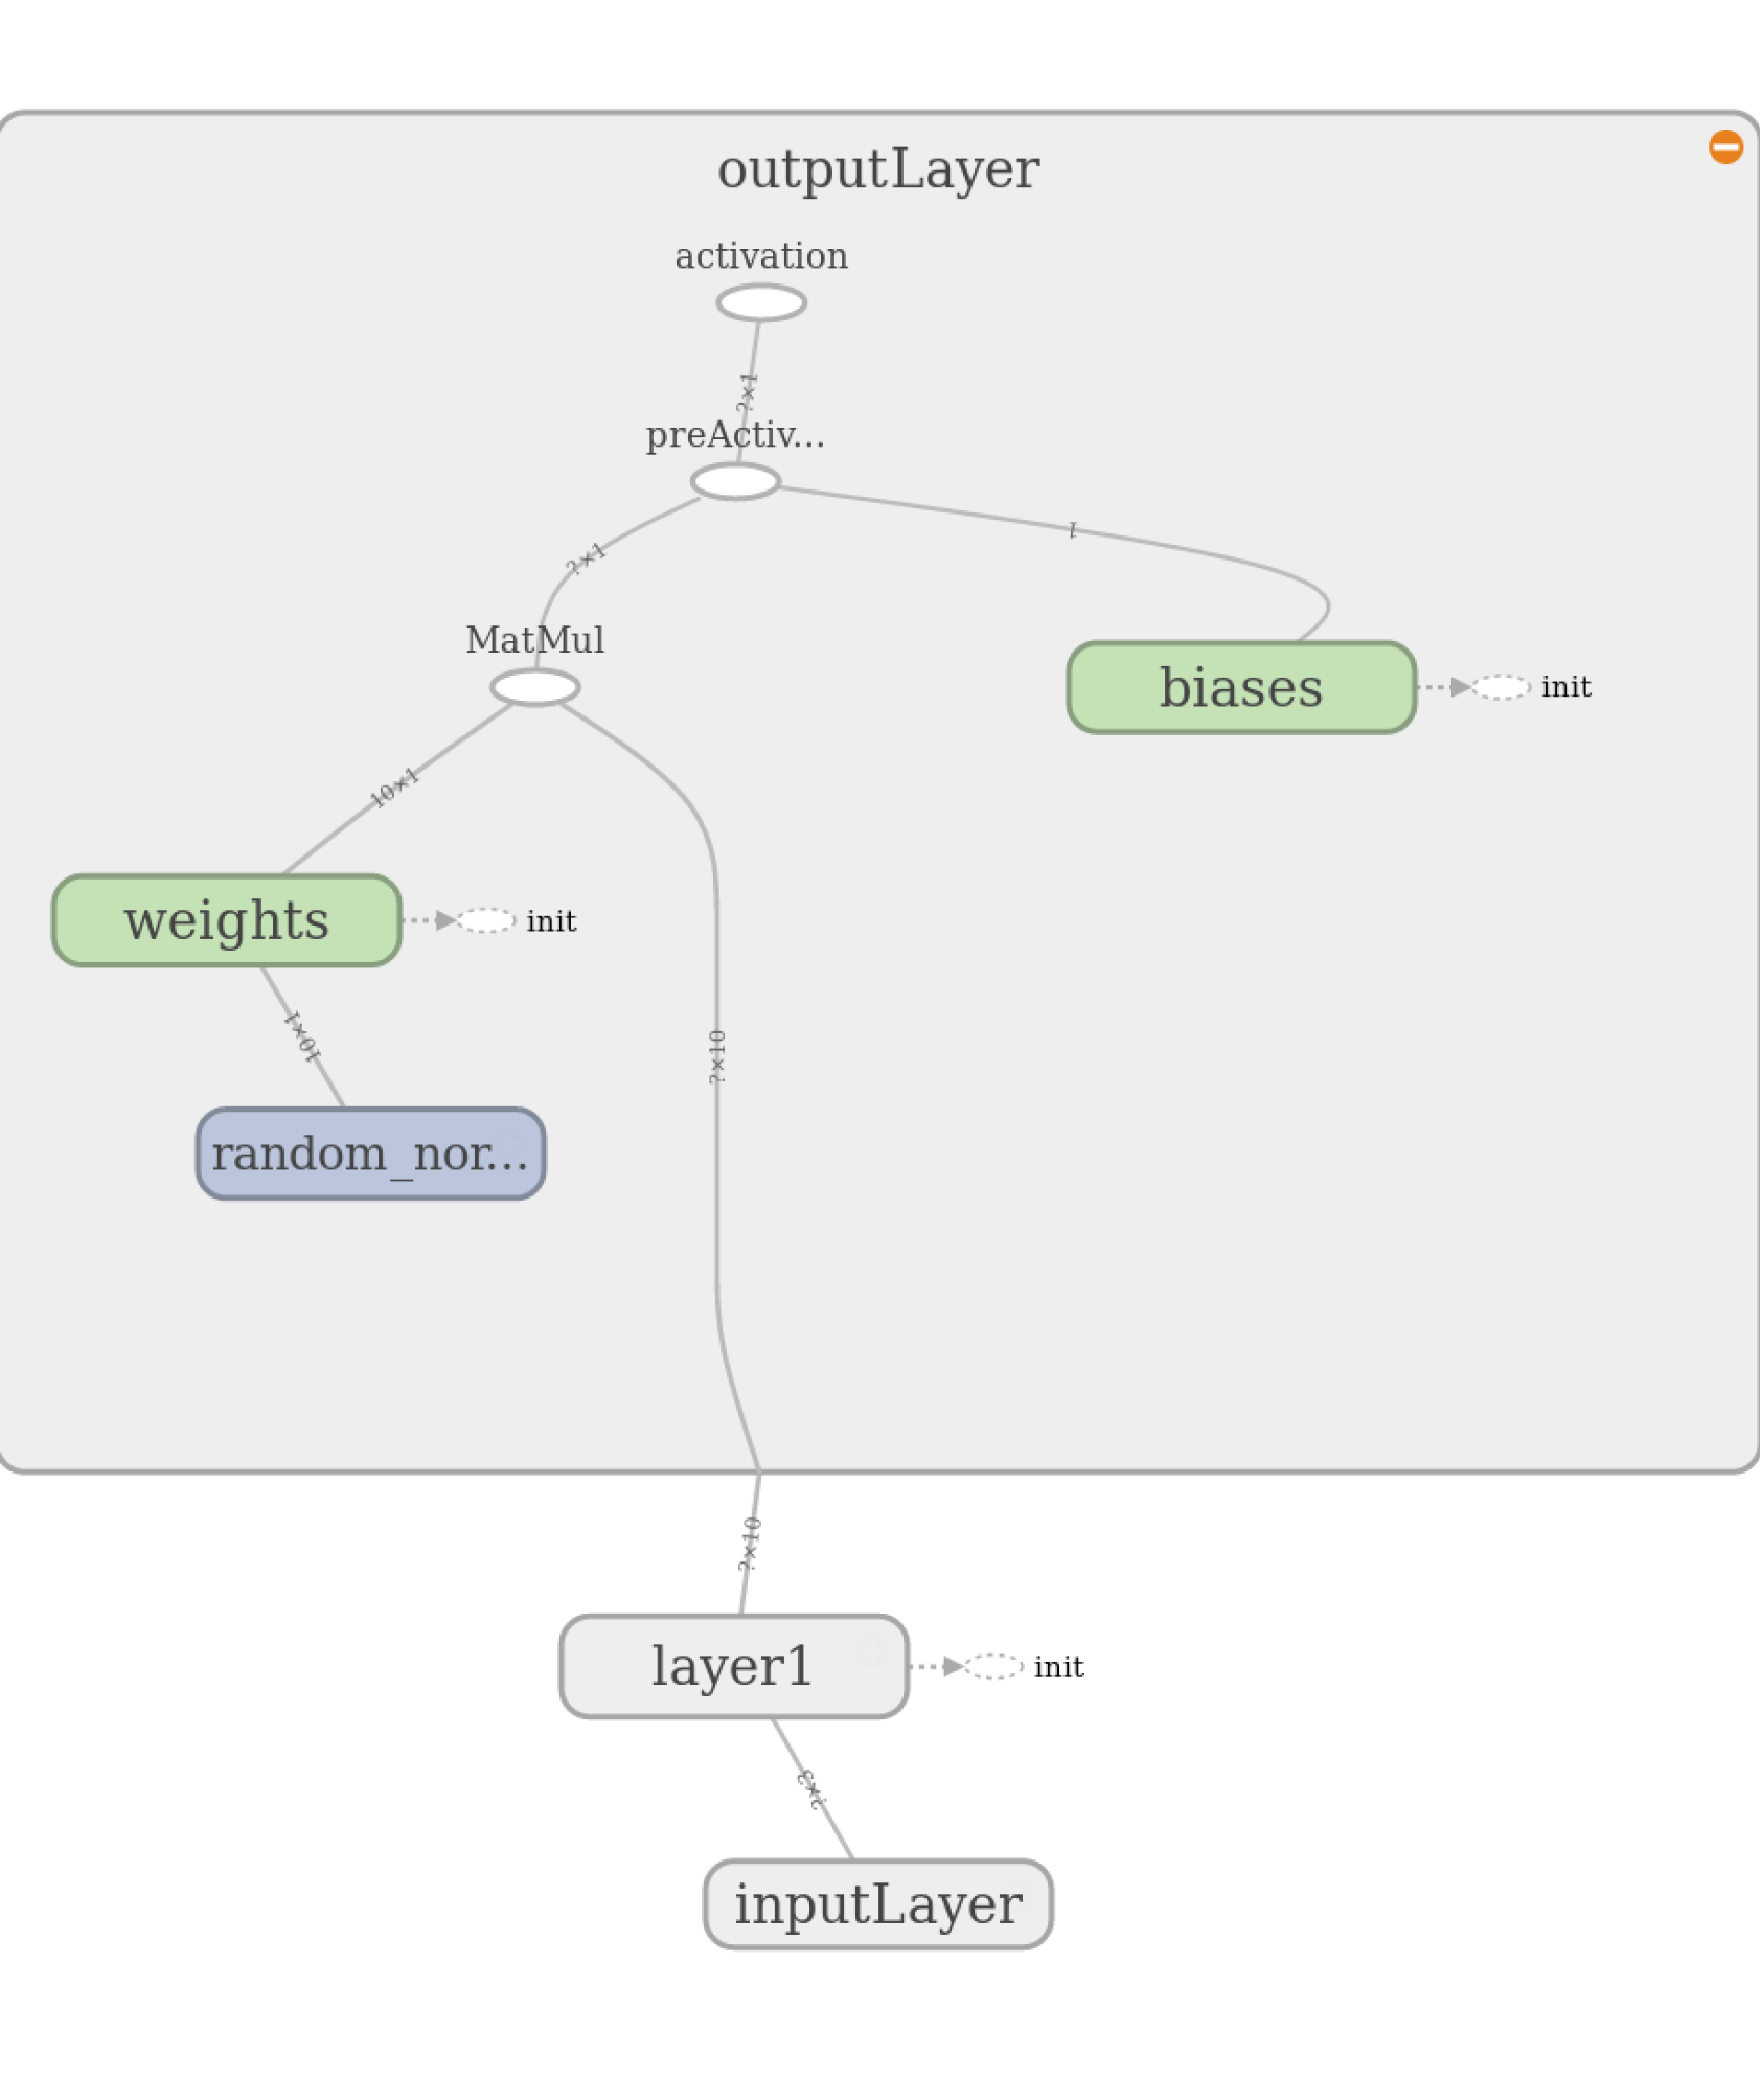
\includegraphics[width=0.7\linewidth]{Figures/Implementation/tensorBoardExample.pdf}
  \caption{Example of a computational graph in TensorBoard of a NN consisting of an input layer, one 
	   hidden layer and an output layer. Nodes are marked by ellipses, the rectangles are namespaces
	   containing several nodes.} 
  \label{fig:graphExample}
\end{figure}
Next, we will demonstrate how to train a NN with TensorFlow. 

\subsection{Training a NN with TensorFlow}
To train the NN described in the previous section, we need two additional components:
a cost function and an optimizer. The mean-square-error cost function \eqref{quadraticCost} is available as a 
built-in function in TF, \texttt{tf.nn.l2\_loss}. To compute the error, we need to supply known 
target values that is fed into a new \texttt{placeholder},
\begin{minted}{python}
 outputData = tf.placeholder(tf.float32, [None,outputs], name='outputData')
\end{minted}
The cost function is now defined as
\begin{minted}{python}
 trainCost = tf.nn.l2_loss( tf.subtract(actOutput, outputData), name='cost')
\end{minted}
This adds an operation to the graph that calculates the mean-square-error between the NN prediction \texttt{actOutput}
on the training data 
and the known target values \texttt{outputData}. In this work, the training data is configurations of atoms, 
while the target values are the atomic energies of these configurations. 

A number of gradient descent-based optimizers are implemented in TensorFlow, including
vanilla gradient descent \eqref{gradientDescent}, Momentum \cite{Qian99}, Adagrad \cite{Duchi11}, 
Adadelta \cite{Zeiler12} and Adam \cite{Kingma14}.
To add the Adam optimizer operation to the graph, we simply write
\begin{minted}{python}
optimizer = tf.train.AdamOptimizer()
trainStep = optimizer.minimize(trainCost)
\end{minted}
To sum up, we have added the following to the script in the previous section (now with name scoping),
\begin{minted}{python}
outputData = tf.placeholder(tf.float32, [None,outputs], name='outputData')

# cost function
with tf.name_scope('cost'):
    error = tf.subtract(actOutput, outputData, name='deviation')
    trainCost = tf.nn.l2_loss(error, name='L2norm')

# optimizer
with tf.name_scope('optimizer'):
    optimizer = tf.train.AdamOptimizer(learning_rate=0.001, name='Adam')
    trainStep = optimizer.minimize(trainCost, name='trainStep')
\end{minted}
\begin{figure}[h]
\centering
  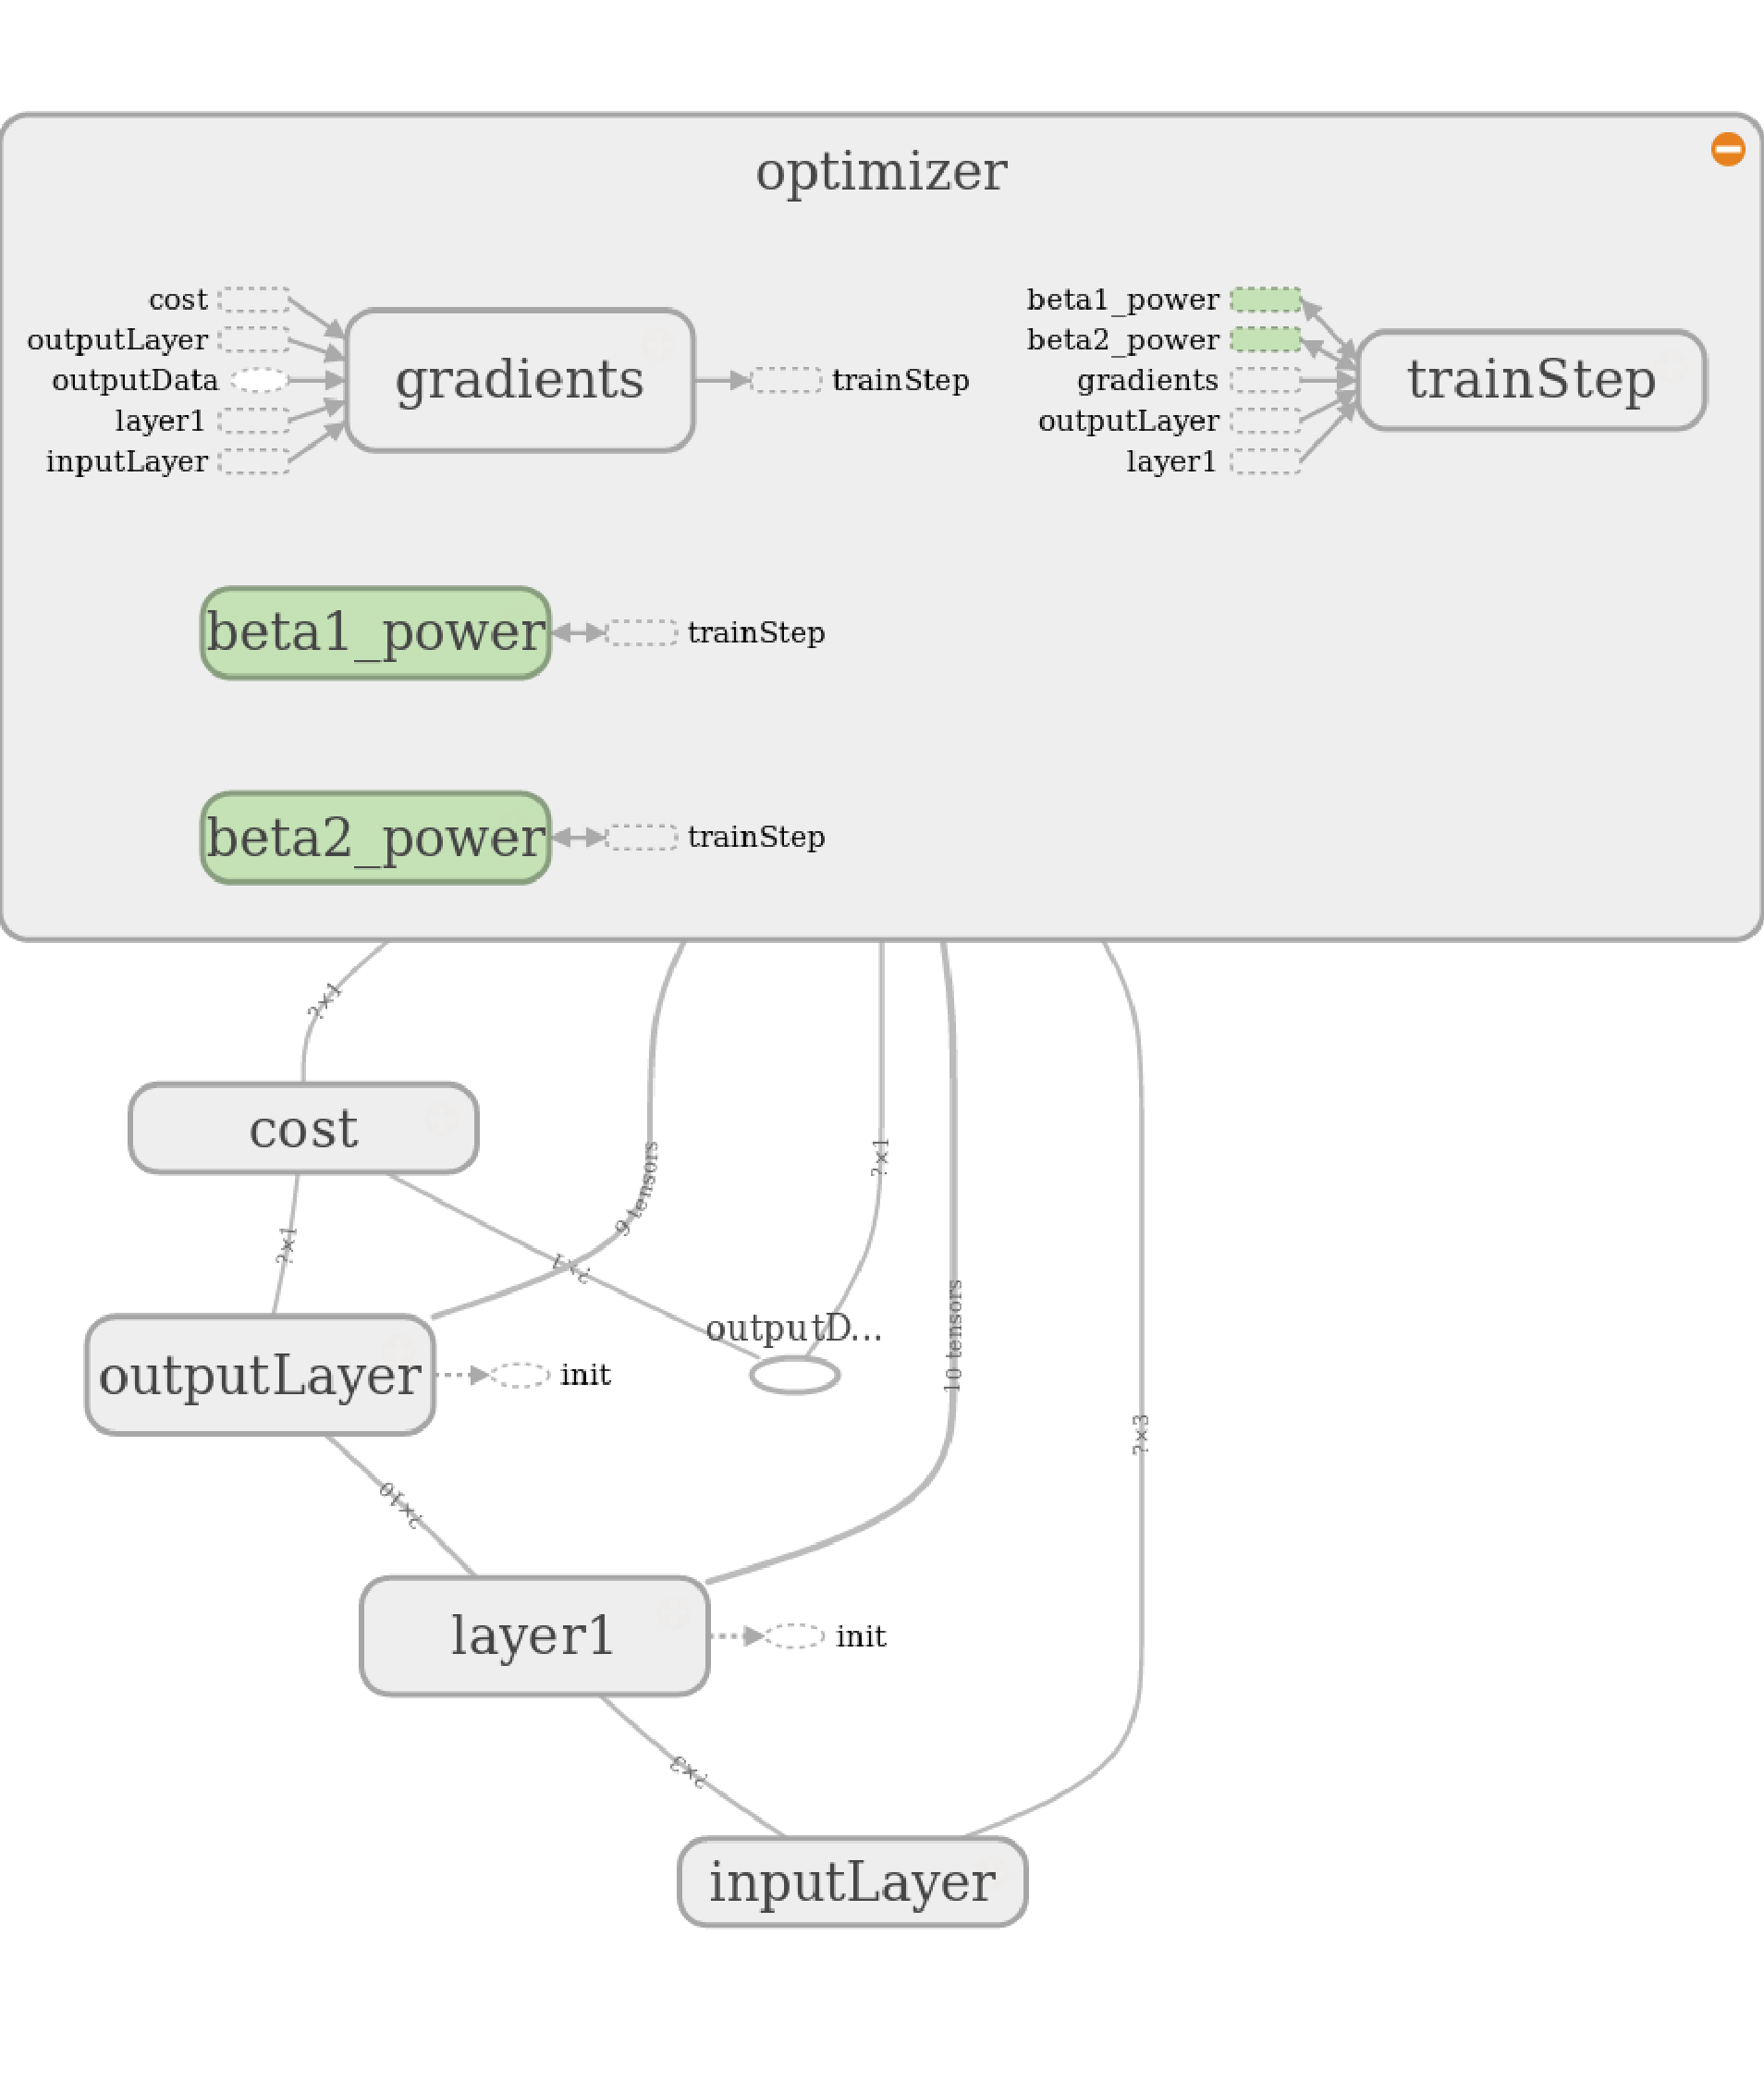
\includegraphics[width=0.8\linewidth]{Figures/Implementation/tensorBoardTraining.pdf}
  \caption{Example of a computational graph in TensorBoard for training a NN consisting of an input layer, one 
	   hidden layer and an output layer. Nodes are marked by ellipses, the rectangles are namespaces
	   containing several nodes. A cost function describing the error of the NN fit and an optimizer that minimizes
	   this error is included in the graph. The optimizer namespace is expanded to display its contents:
	   \texttt{gradients} computes the gradient of all nodes in the graph, \texttt{trainStep} implements
	   the algorithm for updating the NN parameters, while \texttt{beta1\_power} and \texttt{beta2\_power}
	   are the parameters of the Adam optimizer algorithm.}
  \label{fig:tensorBoardTraining}
\end{figure}
The resultant graph can be seen in \autoref{fig:tensorBoardTraining}. 
The optimizer namespace is expanded to display its contents. 
We observe that the optimizer is connected directly to all other parts of the graph, enabling it
to compute the derivative of the cost function with respect to all the weights and biases. This task is
performed by the \texttt{gradients} operation, that in turn sends the total gradient to \texttt{trainStep}, 
which implements the Adam algorithm for updating the NN parameters. 

We are now ready to launch this graph in a training session. We assume that training data
and target values are available as \texttt{NumPy} arrays \texttt{xTrain} and \texttt{yTrain} respectively. 
The code example implements the different variants of gradient descent described in \autoref{sec:gradientDescentVariants}. 
\begin{minted}{python}.
for epoch in xrange(numberOfEpochs+1): 
    
    # for shuffling the training set
    indicies = np.random.choice(trainSize, trainSize, replace=False)
    
    # offline learning / batch gradient descent
    if batchSize == trainSize:    
	
	# pick whole set in random order               
	xBatch = xTrain[indicies]
	yBatch = yTrain[indicies]
	
	# train
	sess.run(trainStep, feed_dict={inputLayer: xBatch, outputData: yBatch})
	
    # online learning / mini-batch gradient descent
    else:                      
	# loop through whole set, train each iteration
	for b in xrange(numberOfBatches):
	    batch = indicies[b*batchSize:(b+1)*batchSize]
	    xBatch = xTrain[batch]
	    yBatch = yTrain[batch]
	    
	    # train
	    sess.run(trainStep, feed_dict={inputLayer: xBatch, outputData: yBatch})
	    
    trainError = sess.run(trainCost, feed_dict={inputLayer: xBatch, outputData: yBatch})
\end{minted}
We observe that the training step is performed with the single line,
\begin{minted}{python}
sess.run(trainStep, feed_dict={inputLayer: xBatch, outputData: yBatch})
\end{minted}
which runs the \texttt{trainStep} operation defined above. This operation initiates a series of
calculations that is performed automatically by TensorFlow. 
First, the NN is evaluated on the training batch \texttt{xBatch} and the output is compared to the corresponding
batch of target values \texttt{yBatch}. The training batch is fed to the NN through the placeholder
\texttt{inputLayer}, while \texttt{outputData} receives the target batch. Next, the cost function 
is calculated, and the error is backpropagated through the DFG to obtain its gradient. Finally, 
the Adam update rule is applied and the weights and biases adjusted. 



\chapter{Constructing a neural network potential} \label{sec:constructingNNP}
In this chapter we present the general workflow for constructing a high-dimensional NNP 
intended for a specific physical application. We describe different ways of assembling 
an adequate training set for the NN, which is the most crucial factor for the performance of 
the final potential. Some of the outlined procedures are primarily used to construct 
\textit{ab inito} NNPs, but are included for reference. 

Next, we discuss how to find a symmetry function set that fits the system under study.
The form of the symmetry functions are found in \autoref{sec:NNsAndMD}, while
the mathematical groundwork of neural networks and various training algorithms are presented in \autoref{sec:machineLearning}.

We start out with a brief discussion on what properties that
are favourable for any PES, irregardless of circumstances. 

\section{What properties should a PES have?}
When developing a new PES, it is important to define a set of properties that the ''ideal'' potential 
should possess. These serve as a guide during the construction process, and is also a good 
starting point for comparing different types of potentials. Behler \cite{Behler15} lists 10 requirements
that the ideal potential should meet, repeated here for reference:
\begin{enumerate}\itemsep1pt
 \item The potential should be accurate, i.e. produce results that are in good agreement with experiments. 
       Ideally, it should be constructed using \textit{ab inito} methods. 
 \item There should be ways to systematically detect situations where the potential is not suffientently accurate, 
       and improve it without too much effort. 
 \item The potential should be unbiased and applicable to all types of systems and chemical bonding. 
 \item The potential should enable the breaking and making of bonds. 
 \item The potential should be high-dimensional, i.e. depend on all degress of freedom of the system. 
 \item The construction of the potential should be as automated as possible. 
 \item The potential should be predictive, i.e. be reliable for atomic configurations that have not been used in the 
       construction. 
 \item The potential should be fast to evaluate. 
 \item The construction of the potential should not require much computation time. 
 \item To compute forces, analytic derivatives of the potential should be available. 
\end{enumerate}
None of the potentials currently available meet all the above requirements to a satisfactory degree. 
At the end of this chapter, we will discuss which of these requirements that are fulfilled by the NNPs constructed
in this thesis. 


\section{Selecting the training data} \label{sec:selectingTrainingData}
The number of possible configurations of atomic or molecular systems quickly grows very large. 
Consider for instance water $\textrm{H}_2\textrm{O}$, which is a three-body molecule. The configuration of the
three atoms can be described by three internal coordinates, each with a certain range of values. 
If each range is divided into $N$ equal segments, the total number of distint configurations is $N^3$. 
If we were to construct an \textit{ab inito} potential that characterizes this system, we would have to compute the energies 
and forces of all these configurations. 
Such a brute-force approach may be feasible for a three-atom molecule, but for more complicated systems
it quickly becomes practically impossible due to the computational cost. 

In this work we do not use \textit{ab inito} methods to compute energies and forces, but this problem is still highly relevant
due to the high-dimensional nature of our approach. The average number of neighbours for the Stillinger-Weber Si simulations
in this thesis is about $n=6$, which is a small number compared to most other systems.  
This number is of great importance to the efficiency of the fitting process because it defines the dimensionality 
of the problem,
\begin{enumerate}
 \item When increasing $n$, each symmetry function is composed of 
 more terms. The number of terms $N_{terms}$ scales like $N_{terms} \propto n$ for the radial symmetry functions, 
 but for the angular symmetry functions we have that $N_{terms} \propto n^2$. 
 \item A larger $n$ leads in general to a larger configuration space to fit, thus additional symmetry functions and 
 a larger data set is required. 
 \item The number of NN parameters must also be increased to obtain the same error as for a lower-dimensional problem
\end{enumerate}
These observations demonstrate that performance is a critical factor whether we fit \textit{ab inito} data or 
not. However, we know that only a small subset of the possible configurations of a system is physically realizable. 
Most of the configurations will not be visited by a system obeying Newton's laws, and are therefore not important to
the dynamics. We thus need some kind of importance sampling method that adequately samples this subset. 
We realize that the obvious way to achieve this is to sample configurations from molecular dynamics simulations, which
yields precisely the subset we are looking for. 

\subsection{Iterative molecular dynamics sampling} \label{sec:iterativeMDsampling}
The method for constructing a NN PES with data sampled from MD simulations is as follows \cite{Behler11general}
\cite{Behler15},
\begin{enumerate}
 \item Sample an initial data set from MD simulations. \label{sample} 
 \item Calculate the energies and optionally the forces of this initial data set with a chosen method. \label{refEnergies}
 \item Train a NN on the data from \ref{sample}. with reference values from \ref{refEnergies}. to
 construct a preliminary NN potential.
 \item Carry out simulations using the NNP to find new relevant structures. 
 \item Compute the energies (and forces) of the new structures with the method from 2. and add them to the data set
 \item Train a NN on the extended data set to improve the NNP
 \item Repeat 4.-6. until a stopping criteria is met
  \label{NNPalgorithm}
\end{enumerate}
The idea is to improve the NN potential iteratively and in a self-consistent 
way by applying it in MD simulations to find 
''holes'' in the data set, i.e. configurations on which the NNP predicts incorrect energies and forces. The process
is different depending on whether we are constructing a NNP from \textit{ab inito} electronic structure data
or reproducing known, empirical MD potentials. 

For the latter, we construct the initial data set by sampling configurations from MD simulations that is relevant
for the intended applications of the NNP. Furthermore, we are extracting both coordinates and energies from the simulations, i.e.
we get both the training data in step 1 and the reference data in step 2 simultaneously. To compute the energies in
step 4, we simply run a pseudo-simulation on the new structures. This is easily done in LAMMPS by using 
the \texttt{rerun} command, which tells LAMMPS to compute the energies and forces of atomic configurations 
supplied from file without doing any integration. 

When constructing an \textit{ab inito} NNP however, we are immediately faced with a problem when trying to execute this process: 
to run MD simulations in step 1 we need the PES we are trying to develop. 
This is often termed as the ''self-starting problem'', 
and several procedures have been suggested for handling it. 

One option is obviously to generate random configurations. This does however take us back to the 
original problem discussed in the beginning of this chapter: the large configuration space volume of
high-dimensional systems enforces the use of importance sampling methods. 
It is highly unlikely that random sampling will yield the important regions of configuration space, thus 
vast amounts of data is needed. Nonetheless, random sampling can be applicable to small systems of 1-3 atoms where
the complete configuration space can be represented without too much effort. 

Another option is to use chemical intuition to select certain configurations of 
the system under investigation. 
For instance, if a specific chemical reaction is studied, one can use previous knowledge about this reaction to 
select configurations along the reaction path \cite{Ischtwan94}. The disadvantage of this approach is that
such information is not always available. 

A more effective method has been presented by Raff et al. \cite{Raff05}, where a semi-empirical
potential has been deployed to initiate the sampling. If a reasonable potential is chosen and an adequate
sampling method is devised (discussed below), several thousand physically relevant structures can be obtained
that will constitue the initial data set. It has also been shown \cite{Raff05} that the final PES obtained 
by the iterative sampling of MD trajectories is not sensitive to the choice of the empirical surface employed 
in the initial step. 

In this thesis we do not construct \textit{ab inito} NNPs, thus we will not go into further details
of the above methods. 

\subsection{Sampling algorithms}
We have seen that MD simulations supply the data that is needed to construct a NN potential, but we 
also have to consider how this sampling should be performed to identify new relevant structures.
NNs have a very flexible functional form which makes them able to accurately fit data sets, 
but they can also yield potentially large energy and force errors 
when evaluated for configurations that are very different from the ones included in the training set.
It is therefore of vital importance to include all structures that are relevant for the intended
application of the NNP.

Sampling methods should in general be optimized to produce a reasonably uniform density of 
data points in those regions of configuration space that are relevant to the application of the fit \cite{Raff12}. 
If there are regions with very high point density compared to others, the NN will be trained to accurately fit these, 
at the cost of regions that are poorly represented. An exception to this rule is regions where the potential gradient, or forces, 
are large. These regions, typically configurations where two atoms are close to each other and experience strong
repulsive forces, are the most difficult for the NN to fit (REFERENCE?), 
and should therefore have a higher density. 

\subsubsection{Initial sampling}
The initial data set is supposed to function as a starting point for the construction of the NNP. 
In this work we use empirical MD potentials to do the initial sampling. Before the process is initiated, 
we must decide on the specific application for the NNP that we want to develop. This entails 
defining a range of temperatures, pressures etc. that the final NNP will be valid for, and sample
configurations based on these. 

The time interval between selecting configurations during the MD simulations must also be decided. 
One alternative is to simply sample points at constant time intervals. This approach will
however result in a non-uniform density of data points considering that atoms spend most of their time
in regions where the forces are small, at least in equilibrium MD. 

To sample configuration space with something close to a uniform density, the time interval $\tau$ between 
sampling needs to be a function of the atomic accelerations (or forces). One such variable 
interval sampling algorithm, suggested by Pukrittayakamee et al. \cite{Pukrittayakamee09}, is given as
\begin{equation}
 \tau = 
\begin{cases}
\textrm{floor}\left[\alpha/a_{\textrm{max}}\right]\Delta t, 
&\textrm{if floor}\left[\alpha/a_{\textrm{max}}\right] > 0 \\
\textrm{floor}\left[\alpha/a_{\textrm{max}}\right]\Delta t + \Delta t, 
&\textrm{if floor}\left[\alpha/a_{\textrm{max}}\right] = 0
\end{cases}
\label{variableIntervalSampling}
\end{equation}
where $a_i$ is the absolute value of the acceleration of atom $i$, $\Delta t$ is the integration step size, 
$a_\textrm{max}$ is the maximum acceleration of a chosen molecule and $\textrm{floor}(x)$ yields
the integer part of $x$. The constant $\alpha$ is system dependent and must be determined empirically. It is the value 
of $\alpha$ that determines the sampling frequency. We see from the second condition in \eqref{variableIntervalSampling} that
configurations with an acceleration $a_i > \alpha$ yields $\tau = \Delta t$, i.e. the shortest possible sampling
interval. On the other hand, if $a_i < \alpha$, the interval increases by a factor $\textrm{floor}(\alpha/a_\textrm{max})$. 
This approach ensures that we sample all configurations where the gradient of the PES is large, while skipping many
of the low-gradient regions of configuration space. 

We have chosen to use the forces $|\vec{F}_i| \propto a_i$ instead of the accelerations, simply because they are
readily available in LAMMPS. When sampling systems with periodic boundary conditions, we have to consider 
the way forces are updated during a simulation. In LAMMPS, any forces attributed to ghost atoms are added back 
to the originals after \textit{all} forces are computed. This is done in
\texttt{verlet.cpp},
\begin{listing}[H]
 \begin{minted}{c++}
  if (pair_compute_flag) force->pair->compute(eflag,vflag);
  // ...
  if (force->newton) comm->reverse_comm();
 \end{minted}
\end{listing}
The first line computes the forces on all atoms with the chosen \texttt{pair\_style} potential, while
the second line communicates the forces on ghost atoms back to the original atoms according to Newton's third law. 
This means that to employ the algorithm
\eqref{variableIntervalSampling}, we need to sample configurations \textit{after} this reverse communication is
executed, if not the forces will be incorrect. This can be achieved by extending LAMMPS with a new \texttt{compute} 
(described in \autoref{sec:extendingLammps}), as all \texttt{computes} and \texttt{fixes} are invoked after the
force calculations. 

We have made an additional modification to the algorithm \eqref{variableIntervalSampling}.  
Pukrittayakamee et al. \cite{Pukrittayakamee09} sample \texttt{clusters} of atoms for subsequent DFT calculations
of the energies of these clusters, and computes $\tau$ based on the maximum acceleration of an atom in a cluster. 
Our strategy is to select a few atoms, usually 1-10, and compute $\tau$ seperately for each of these atoms. When 
the sampling criterium is met, the coordinates of all neighbours relative to the central atom is written to file, 
as well as the atomic energy the central atom experiences in the presence of its neighbours. These coordinates
and energies make up the training data and reference values, respectively, for a NN to interpolate. 
Our modified sampling algorithm is thus as follows (written in a less convoluted way than above),
\begin{equation}
 \tau = 
\begin{cases}
  \textrm{floor}\left[\alpha/F_i\right], &F_i \leq \alpha \\
  1, &F_i > \alpha \\
  \tau_\textrm{max}, &\textrm{floor}\left[\alpha/F_i\right] > \tau_\textrm{max}
\end{cases}
\label{samplingAlgorithmModified}
\end{equation}
where $\tau$ is measured in units of $\Delta t$ and $\tau_\textrm{max}$ is the maximum value of $\tau$.
$F_i$ is the total force on atom $i$ including ghost contributions. 
We have implemented this sampling algorithm as follows,
\begin{listing}[H]
\begin{minted}{c++}
// ...
// loop through atoms that is to be sampled
for (auto ii : chosenAtoms) {
    i = ilist[ii];
    itype = type[i]-1;

    double F = sqrt(f[i][0]*f[i][0] + f[i][1]*f[i][1] + f[i][2]*f[i][2]);

    // update tau every maxDelay step
    if ( !(myStep % maxDelay) ) {

      // no delay if force is larger than alpha
      if (F > alpha[itype]) tau[atomCount] = 1;

      // calculate delay if force less than alpha
      else {
        int factor = floor( alpha[itype] / F );
        if (factor > maxDelay) tau[atomCount] = maxDelay;
        else                   tau[atomCount] = factor;
      }
    }

    // decide whether to sample or not based on current value of tau for atom i
    if ( (myStep % tau[atomCount] > 0) && useAlgo) continue;

    double xi = x[i][0];
    double yi = x[i][1];
    double zi = x[i][2];
    
    // loop through neighbours of atom i 
    // write relative coordinates and atomic energy to file
    jlist = firstneigh[i];
    jnum = numneigh[i];
    for (jj = 0; jj < jnum; jj++) {
      j = jlist[jj];
      // ...
\end{minted}
\end{listing}
The vector \texttt{chosenAtoms} contains the indicies of the atoms that are to be sampled. These indicies are decided
when the parameters of the employed potential is initiliazed with the input script command \texttt{pair\_coeff}. 
The variable \texttt{maxDelay} decides how often $\tau$ is updated, and functions as a maximum value of $\tau$. 
Its value does not change in the course of the simulation. 
\begin{figure}[H]
\begin{minipage}[t]{0.48\linewidth}
  \subcaption{}
  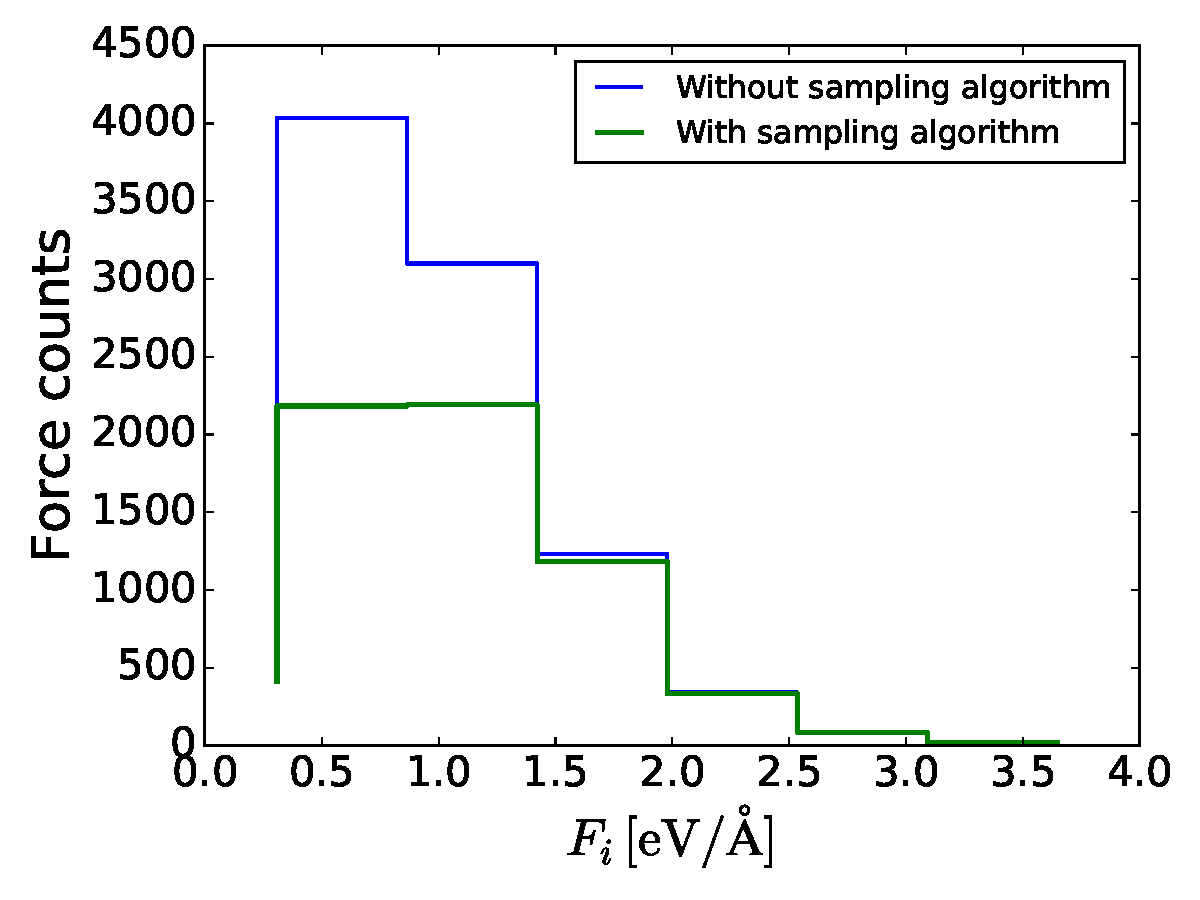
\includegraphics[width=\textwidth]{Figures/Implementation/forceDistSamplingAlgo.pdf}
\end{minipage}
\quad
\begin{minipage}[t]{0.48\linewidth}
\subcaption{}
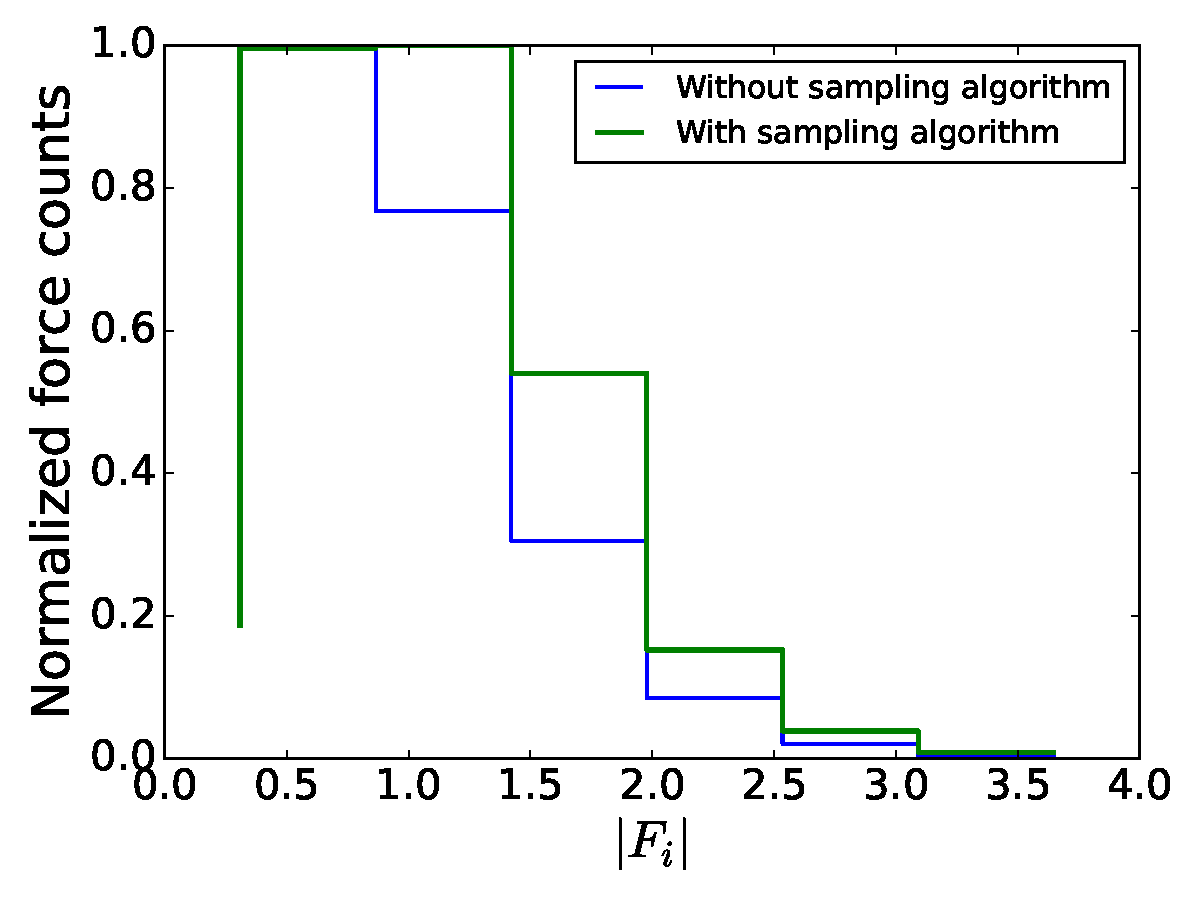
\includegraphics[width=\textwidth]{Figures/Implementation/forceDistSamplingAlgoNormed.pdf}
\end{minipage}
  \caption{Distribution of forces for one Si atom in a quartz $\textrm{SiO}_2$ crystal with 
	   and withouth the use of the sampling algorithm \eqref{samplingAlgorithmModified}. 
	   The crystal consists of 576 atoms, with an initial temperature $T= \SI{1000}{\kelvin}$, 
	   run for $N = 10000$ time steps. The atoms are sampled from the microcanonical ensemble with
	   periodic boundary conditions.
	   Sampling algorithm parameters: $\alpha=3.0$ and 
	   $\tau_\textrm{max} = 10$.}
\label{fig:forceDistSamplingAlgo}
\end{figure}
\autoref{fig:forceDistSamplingAlgo} displays the distribution of forces for one Si atom in a MD simulation
of quartz $\textrm{SiO}_2$, with and withouth the use of the sampling algorithm \eqref{samplingAlgorithmModified}. 
We see from the figure a) that the sampling procedure cuts the number of low-gradient configurations significantly, 
while keeping all the environments corresponding to large forces. The resulting distribution is however not uniform, simply
because the ratio of force counts in the range $F_i = \SIrange{0}{2}{\angstrom}$ to the range $F_i = \SIrange{2}{4}{\angstrom}$
is too high originally.

One way to smooth the distribution further is to manually delete configurations after the simulation 
is finished, but then we risk removing relevant structures. The gradient of the PES is not the only way 
to measure the quality of the sampled set, the time aspect is also important. 
By selecting samples on-the-fly, we are guaranteed that the they are distributed somewhat uniformly in the time domain. 
Deleting structures blindly subsequent to the simulation is therefore not a good idea (I AM NOT SURE IF THIS IS TRUE, 
HAVE TO BE TESTED).

Another option is to sample different types of systems where the forces are more evenly distributed. 
Examples are non-periodic systems or systems containing only a few atoms. Also, it can be a good idea 
to do short simulations where the atoms start out in non-equilibrium positions to obtain configurations
that are not visited by systems with a regular lattice initial state. 
In general, it is not required that the data used to train the NNs are the results of physically plausible 
simulations, the only requirement is that it should cover all possible configurations that the NNP have the possibility
of experiencing in the course of its application. WRITE MORE / DO TESTS ON THIS???

\subsubsection{Iterative sampling}
The initial data set is usually not sufficient to construct a stable neural network PES. 
It is difficult to identify all the relevant structures that the NN have to learn to perform well, and 
since there is always a small fitting error, the 
NNP will generate different trajectories than the PES that has been used to train it. This is solved
by sampling new relevant structures from simulations using the preliminary NNP trained on the initial data set. 
In this way, new configurations
will ''naturally present themselves'', and the NNP will iteratively improve in a self-consistent way.

The obvious way to identify new structures not already in the initial data set is to evalate both the NNP and 
the PES we are trying to fit for each structure in an NNP MD simulation and compare the energies (and eventually 
the forces). If the energy deviation is above a certain treshold, the structure is added to the training set.
The simulations should be carried out under the conditions of the intended application of the NNP to ensure
that the relevant parts of configuration space are sampled.
After a certain amount of new data is added, 
the NN is trained on this extended data set and thus improved. Then, new simulations are carried out with the improved
NNP and so on, according to the iterative process \autoref{NNPalgorithm} described in the beginning of this chapter. 

This approach is easily feasible when the target PES is an empirical potential, but too computationally expensive 
in the case where electronic structure methods are employed. Raff et al. \cite{Raff05} have developed a sampling
algorithm called \textit{modified novelty sampling} that does not require any quantum mechanical calculations of
the energies of new structures. They describe the database as a set of vectors $\{\vec{q}\}$, where vector
$\vec{q}_i$ contains the internal coordinates of the $i_\textrm{th}$ cluster of atoms. New configurations
$\vec{q}_n$ are generated using the NNP trained on this data base and the 2-norm difference $\vec{d}$ between vectors
$\vec{q}_n$ and $\vec{q}_i$ are computed,
\begin{equation}
 \vec{d} = | \vec{q}_i - \vec{q}_n | = 
 \left[(\vec{q}_i - \vec{q}_n)\cdot(\vec{q}_i - \vec{q}_n)\right]^{1/2}
\end{equation}
for all clusters $i$. The difference vector is characterized by its minimum value $d_\textrm{min} = \textrm{min}(\vec{d})$ and 
the mean seperation distance $d_\textrm{mean} = \langle\vec{d}\rangle$. 
The basic idea is to add configuration point $\vec{q}_n$ to the database with high
probability if $d_\textrm{min}$ or $d_\textrm{mean}$ is large, but low probability if both 
$d_\textrm{min}$ and $d_\textrm{mean}$ are small. The energy output of the NNP are also included in the scheme, along with
a more involved selection algorithm. As this thesis only deals with empirical target potentials, the details will
not be further discussed here. 

In this work we use the Behler symmetry functions to transform atomic cartesian coordinates to vectors of symmetry values.
These functions act as descriptors of chemical environments, and should therefore be excellent candidates
to identify relevant structures during MD simulations without computing additional target energies. 
Behler has suggested two methods \cite{Behler11general} where these symmetry functions are employed to improve the NNP. 
The first and simplest method identifies structures that fall outside of the range of input values spanned by the training data. 
This is achieved by comparing the symmetry function vector of each atom during the MD simulation with 
the minimum and maximum values of each symmetry function in the database for the respective element. 
When such configurations are encountered, a warning can be issued and the structure sampled.  

The other method developed by Behler is called the \textit{multiple-NN method} and are used to identify 
structures that are within the range of existing symmetry values, but located
in parts of configuration space that are poorly represented in the training set.
The idea is to use the high flexibility and reasonably fast training and evaluation of NNs to validate 
the potential. The procedure is as follows,
\begin{enumerate}
 \item Fit several NNs with different architectures to the same training set. All the NNs should be trained
 to the same accuracy. 
 \item Generate a large number of trajectories and corresponding energies using one of these NNPs in MD simulations.
 \item Recalculate the energies of the obtained trajectories using the other NNPs
 \item Structures for which the energy disagreement between the different NNPs is significant should be added to 
 the training set.
\end{enumerate}
This method takes advantage of the poor extrapolation abilites of NNs: the energy predictions of the different NNPs will
be more or less random on structures that are far away from the training points. Thus, missing structures can 
be identified by comparing the energy predictions of the different NNPs on the genereated trajectories. The procedure 
also provides a criterion for determining the convergence of the PES without requiring the repeated computation 
of dynamic properties of the system under study. When, after several iterations of the multiple-NN method,
no problematic structures are found, the NNP should be reliable and ready for use. 

\subsubsection{Summary}
In this section we have presented the workflow for constructing a NNP, including several procedures to 
assemble the training set for the NN, which depends on how the target energies are computed. 
In this work, we know the PES we are trying to fit, which are well-known empirical MD potentials. 
Therefore, the NNP is validated simply by comparing its predictions to the target PES.  
On the other hand, if an \textit{ab inito} NNP is to be constructed, the underlying target PES is not known, 
and computing energies and forces of eventual new structures are expensive. Two methods circumventing
this problem has been described, but they are not used in this thesis. 

Still, there are several factors to consider when constructing the training set, irrelevant of how the target PES looks like.  
We have implemented and employed the sampling algorithm \eqref{samplingAlgorithmModified} in this thesis to obtain a more uniform
distribution of forces in the data set. The thermodynamical properties of the MD simulations that we sample configurations 
from have also been carefully considered, described in more detail in \autoref{sec:SiPotentialResults}.  



\section{Constructing the symmetry function sets} \label{sec:constructingSymmetry}
The choice of symmetry functions is important to achieve a good fit to the reference data. 
They need to be able to sufficiently distinct inequivalent structures to avoid fitting 
contradictory data. If this distinction is not possible, different reference structures with 
different energies and forces give rise to the same symmetry function values, which results in poor fits. 

Although a NN potential is general and unbiased because it has no pre-defined functional form, the 
construction of the symmetry function sets is to some extent empirical. The functional form of the NN
is adjusted ''automatically'' when trained, while the symmetry function set has to be constructed manually.
This observation does however not change the fact that the high-dimensional neural network approach to
constructing potentials used in this work is general, and can in principle be applied to any system. The training data
and symmetry function sets have to be customized to each system, but the overarching procedure is the same. 

\subsection{Initial set}
There are some general rules that guide the construction of the symmetry function set. \cite{Behler15}
\begin{enumerate}
 \item The symmetry function set should cover the configuration space in an unbiased way. 
 \item The range of the radial symmetry parameters should correspond to the range of inter-atomic distances in the data set.
 \item The set of values of two different symmetry functions on a given data set should not be strongly correlated. 
 \item The symmetry function set should be as small as possible.
 \item For each symmetry function, the range of function values should be as large as possible.   
\end{enumerate}
1. can be realized by simply choosing an equidistant set of initial radial symmetry functions.
Further, the distribution of inter-atomic distances in the data set may be investigated to aquire a 
lower and upper bound on the range of radial parameter values (2.). For $G^2$, a rule of thumb is that, for each element, 
the width (standard deviation) of the Gaussian
with the largest $\eta$ value should correspond to the shortest inter-atomic distance present in the data set 
and vice versa. Also, a set of symmetry functions with equidistant $R_s$ parameters should be present in the initial set.
These should all have the same (large) $\eta$ value. An example of such an initial radial symmetry function set is displayed
in \autoref{fig:radialParams}. 
\begin{figure}
\centering
  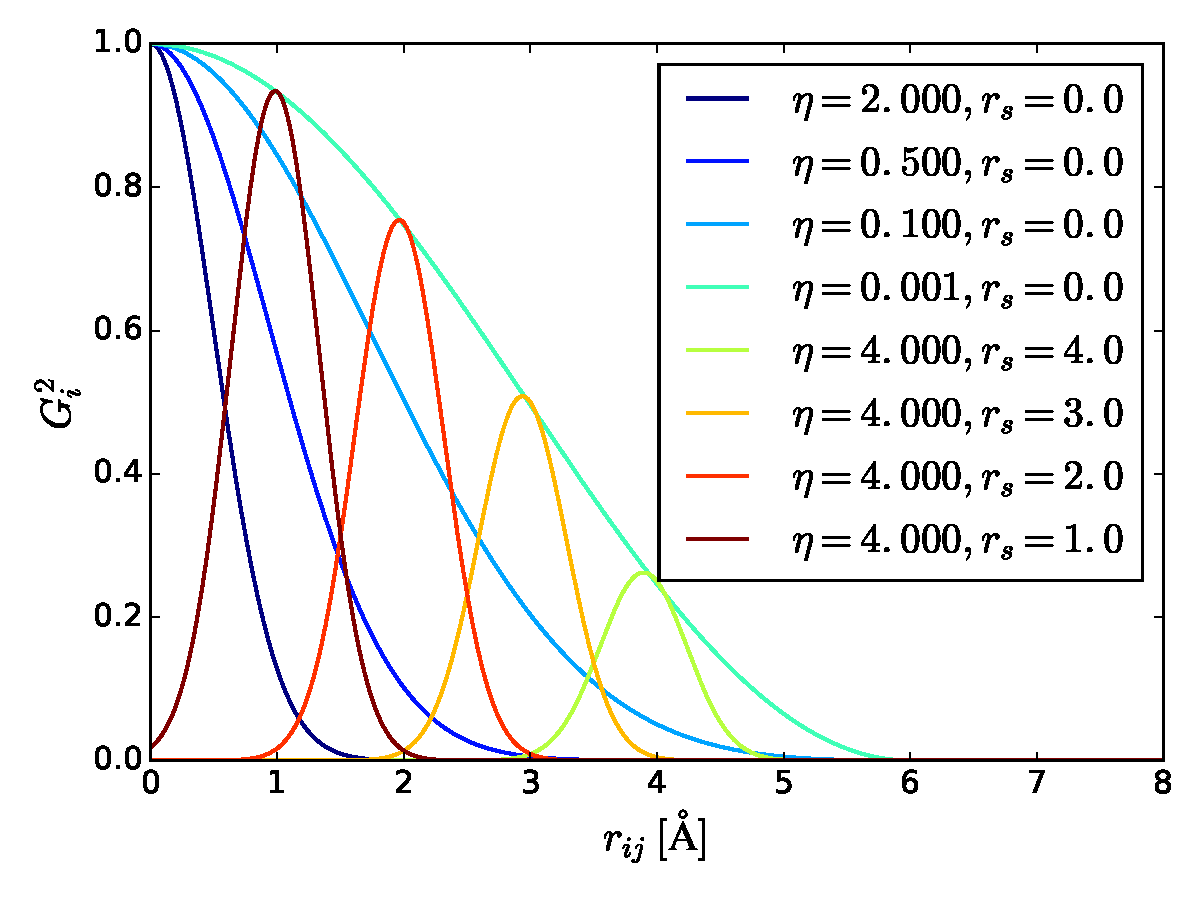
\includegraphics[width = 0.7\linewidth]{Figures/Implementation/radialParams.pdf}
  \caption{Example of an initial radial symmetry function set. The parameters $\eta$ and $R_s$ are varied to 
  probe the radial arrangement of neighbouring atoms.
  All symmetry functions have the same cutoff $R_c = 6.0$. 
  $R_{ij}$, $R_s$ and $R_c$ are in units of $\SI{}{\angstrom}$, while $\eta$ have units $\SI{}{\angstrom}^{-2}$.}
  \label{fig:radialParams}
\end{figure}

A set of initial angular symmetry functions can be made in a similar way. 
The angular distribution of neighbours is probed by varying $\zeta$ and $\lambda$ at differing radii, i.e. for 
several values of $\eta$ and/or $R_c$. 
We have found from empirical investigations that fixing $\eta$, while varying $R_c$ yield the best results. 
In contrast to the radial parameters, the set of $\zeta$ parameters should not be equidistant. Instead, the values of $\zeta$
should increase exponentially to ensure that the symmetry functions are sufficiently dissimilar (3.). An example is shown in 
\autoref{fig:angularParams}. 
\begin{figure}
\centering
  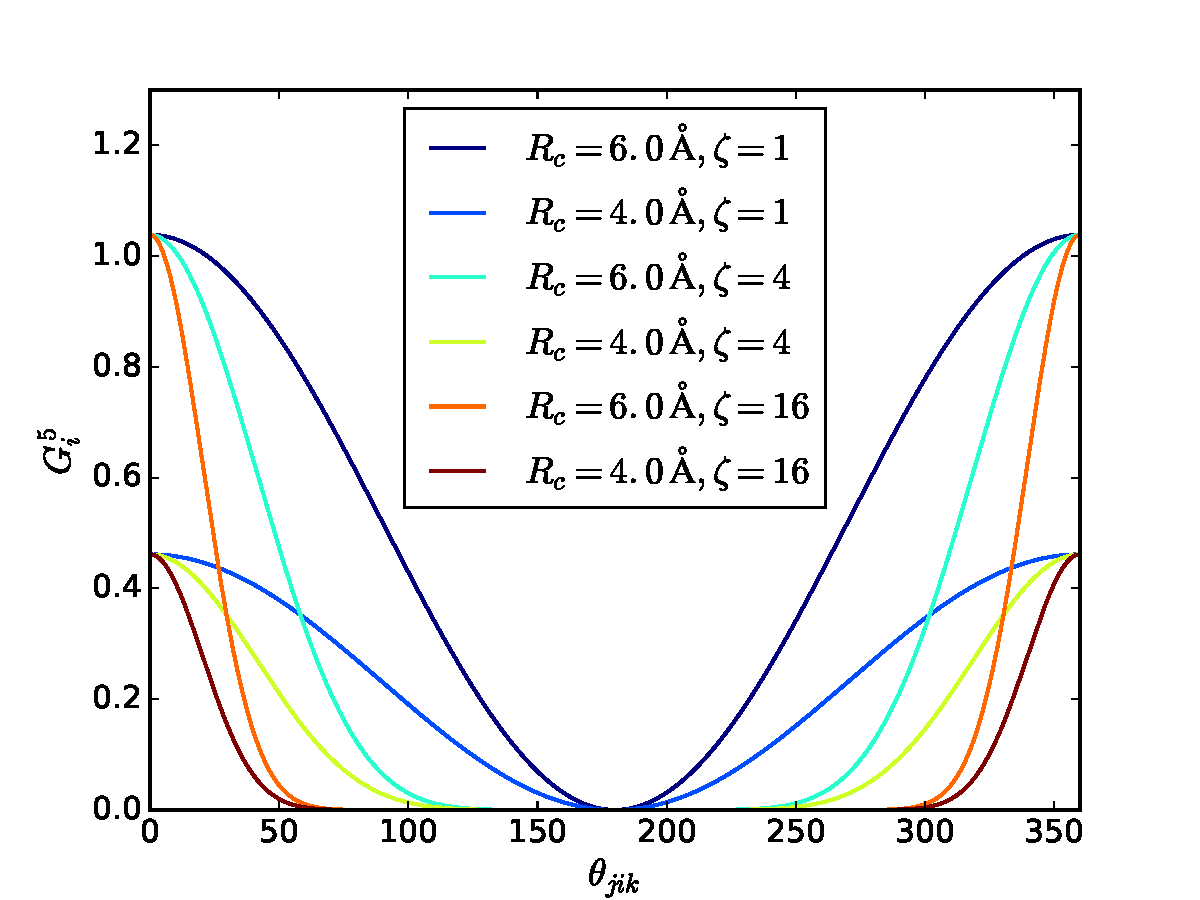
\includegraphics[width = 0.7\linewidth]{Figures/Implementation/angularParams1.pdf}
  \caption{Example of an initial angular symmetry function set
  with $\eta = \SI{0.01}{\angstrom}^{-2}$ and 
  $\lambda = 1$. A corresponding set of functions with $\lambda = -1$ should also be added to make the set more complete. 
  The $\zeta$ parameter is increased in a non-linear way to avoid excessively overlapping functions. }
  \label{fig:angularParams}
\end{figure}

\subsection{Adjusting the set}
Thus, 1., 2. and 3. can be used as a framework for constructing an initial set of symmetry functions.
Then, we carry out various analyses to investigate whether our chosen symmetry functions 
adequately probe the configuration space defined by the data set. Item 3., 4. and 5. above serve as the
guiding principles for the analyses. 

\subsubsection{The range of each symmetry function}
Using 5., the range of values for each symmetry function should be obtained. Each symmetry function
assigns \textit{one} numerical value to each training example. If the range of a symmetry function is too small, 
the difference between the function values for distinct structures will also be small. Consequentially, 
the NN will try to assign substantial energy changes to tiny changes in the symmetry function, which 
can lead to numerical instability. 

This can be avoided by analyzing the distribution of values of each symmetry function on the data set. If the difference 
between the maximum and the minimum function value is below a certain threshold
the symmetry function should be removed or its parameters changed. Specifically, 
symmetry functions which have a value of zero for all configurations should be avoided, as these will not contribute
to the description of the chemical environments. 

\subsubsection{Correlations}
There is a trade-off between the ability of the symmetry function set to cover the configuration space and 
the efficiency of the calculation of the NN energy output. The number of symmetry functions can be kept as low as 
possible (4.) by calculating the correlation between the values of two different symmetry functions for the whole 
training set (5.). If there is a large correlation, the two symmetry functions are almost linearly dependent, 
and we have a redundancy of information. Consequentially, one of them should be removed, or the parameters adjusted
to decrease the correlation.

To demonstrate how the correlations can be calculated, we remember that in 
\autoref{sec:training} the training set was represented as a matrix $X$, where
each row is a training example, in this case the values of all the symmetry functions for a single atomic configuration.
We can calculate the correlations between each pair of symmetry functions with the \texttt{NumPy} method \texttt{corrcoef}, 
\begin{minted}{python}
  R = np.corrcoef(np.transpose(X))
\end{minted}
The training set matrix $X$ is transposed because \texttt{corrcoef} expects each \textit{row} to represent all the samples of one
variable (function), while each \textit{column} is a single observation of all the variables.
A matrix $R$ is returned where the $(i,j)$-th element is the Pearson correlation coefficient between 
symmetry function $i$ and $j$,
\begin{equation}
 R_{ij} = \frac{C_{ij}}{\sigma_i\sigma_j}
\end{equation}
where $C$ is the covariance matrix and $\sigma_i$ is the standard deviation of the values of symmetry function $i$ for 
the whole training set. Pair of functions which are strongly correlated can thus be identified and altered. 


\section{Summary}
In the beginning of this chapter we listed 10 properties that an ideal potential should possess. 
We are now in a position to evalute the NNPs constructed in this thesis in the light of these requirements. 
\begin{enumerate}
 \item The NNP can be fitted to \textit{ab inito} data to arbitrary accuracy, and 
       can therefore be considered to have \textit{ab inito} accuracy.  
 \item The NNP can be systematically improved by employing the iterative scheme proposed in \autoref{sec:iterativeMDsampling}.
 \item The potential is unbiased, and its applications are unlimited as long as the production of \textit{ab inito} reference energies
       is feasible. 
 \item The potential is able to model the breaking and making of bonds as long as the training set is sufficiently comprehensive.  
 \item The potential is high-dimensional because it depends on all the degrees of freedom of the chemical environment of each atom. 
 \item The training of the NN is automated, but there are a number of parameters that needs to be set manually. 
       The training set must also be assembled with care. 
 \item The potential is generally not able to extrapolate. 
 \item The potential is several orders of magnitude faster to evalute than e.g. DFT or Hartree-Fock potentials, but notably 
 slower compared to empirical potentials like Lennard-Jones or Stillinger-Weber. 
 \item Training does not require much computation time, but calculating reference energies for thousands of configurations
 is time consuming. 
 \item Analytic derivatives for force computations are readily available. 
\end{enumerate}



\chapter{Validation}

\section{Time usage} \label{sec:timeUsage}
The workflow when training a NN and using it in MD is as follows: 
\begin{enumerate}
 \item Generate training data
 \item Train a NN to fit the data
 \item Use the analytical expression for the trained NN as a potential in MD
\end{enumerate}
The main application programming interface (API) for TensorFlow (TF) is Python. The NN is therefore
trained using Python scripts, while C++ is utilized to run the MD simulations for speed purposes. Thus
we need a way to transfer the NN from Python to C++. 

There are built-in functions in TF that automatically saves computational graphs (architecture of network plus
nodes for training) and variables (weights and activation functions) as binary files.
These files can then be read and the NN evaluated using the TF C++ API. This API is however quite under-developed
and the documentation is very sparse. Another alternative is to manually save the weights and biases
as a text file, along with information on which activation function(s) that has been used. This file 
file can then be used to reconstruct the NN in the same way that it is made in Python: By representing
the connection weights between layers as matrices and the biases as vectors. The activation functions
must be coded manually. A linear algebra library should
be utilized for speed and simplicity; we have chosen to use Armadillo. 

To find out which alternative is the most efficient for evaluating a NN, we compare the 
time usage in three cases: with TF in Python, with TF in C++ and with Armadillo. 
The results are shown in \autoref{fig:timeComparisonEvaluateNetworkTotalScatter}.
\begin{figure}[H]
\centering
  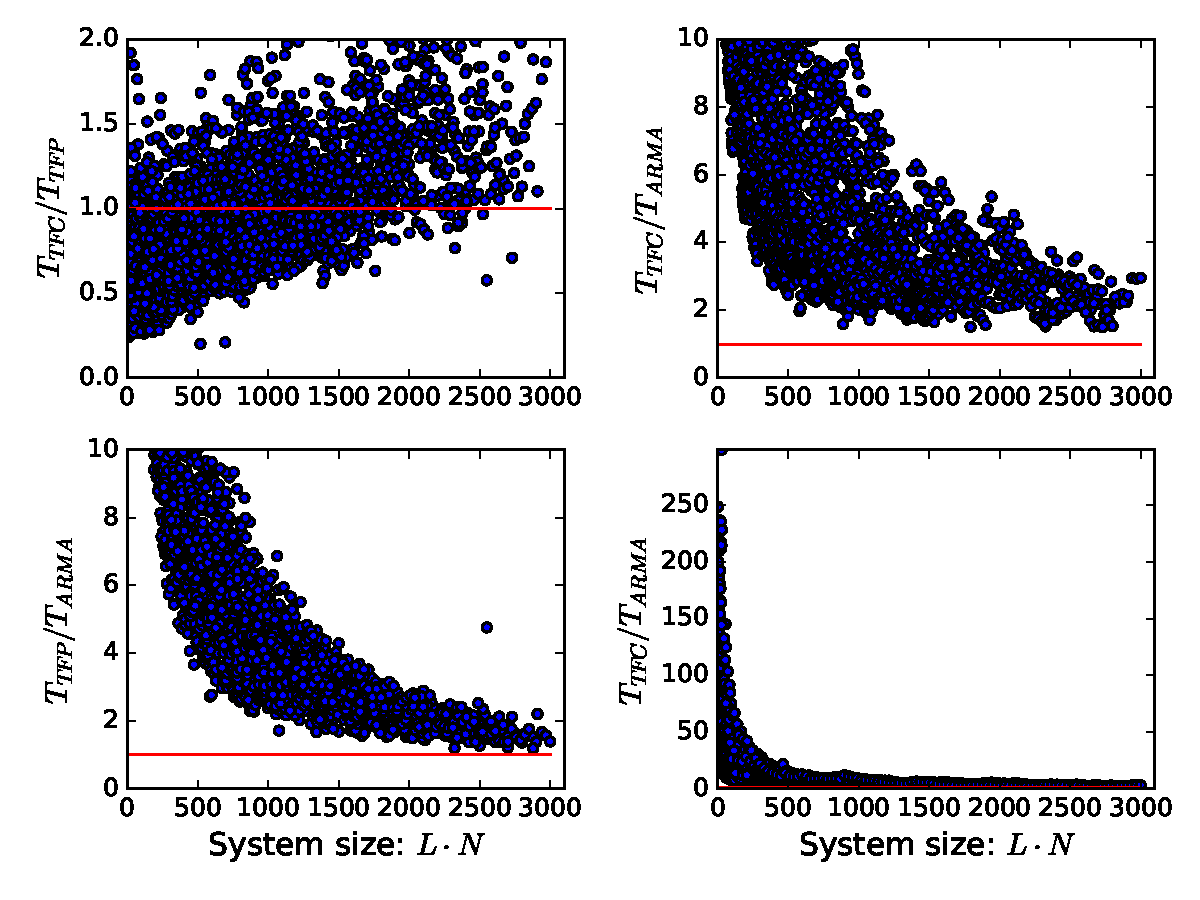
\includegraphics[width = 0.9\linewidth]{Figures/Tests/timeComparisonNetworkTotalScatter.pdf}
  \caption{Scatter plot of CPU time when evaluating untrained NNs with random weights and sigmoid activation functions
	   using the TF Python API ($T_{TFP}$), the TF C++ API ($T_{TFC}$) and Armadillo ($T_{ARMA}$). 
	   $L$ is the number of layers, $N$ is the number of nodes in each hidden layer. All the NNs
	   have one input and one output. The time has been found by averaging over 50 evaluations
	   for each NN architecture. $T_{TFC}/T_{ARMA}$ is also shown in an uncut version to demonstrate
	   how large the time difference is for very small NNs.}
\label{fig:timeComparisonEvaluateNetworkTotalScatter}
\end{figure}
\begin{figure}[H]
\centering
  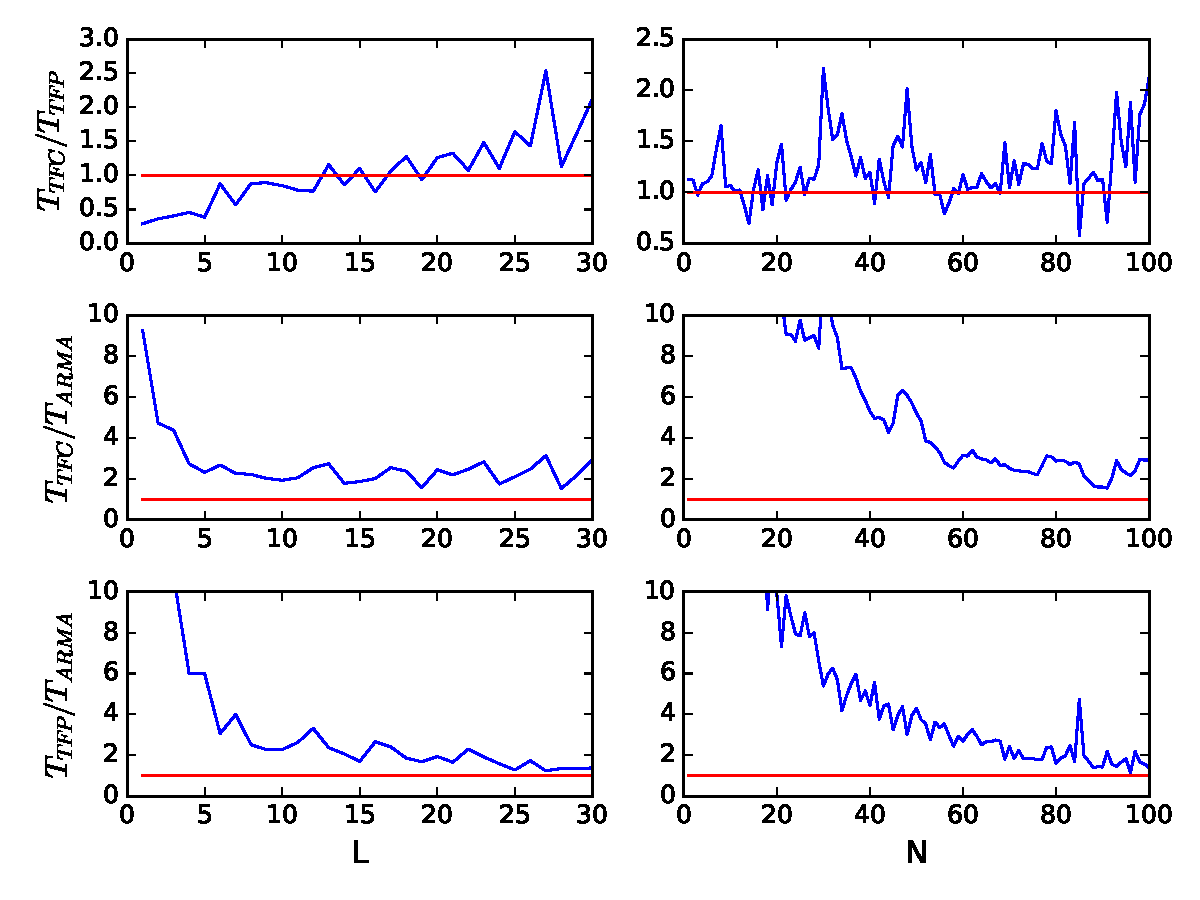
\includegraphics[width = 0.9\linewidth]{Figures/Tests/timeComparisonNetwork3.pdf}
  \caption{Left column: CPU time comparison for $N=100$. Right column: CPU time comparison for $L=30$.} 
  \label{fig:timeComparisonEvaluateNetwork2}
\end{figure}
As we can see, evaluation of an NN with the built-in TF methods are notably slower than with Armadillo 
for small NNs, but seems to converge to 1 for large networks. The convergence rate is however surpisingly low. One reason for this
can be that the \textit{Session} environment in TF has lot of overhead. However, the main computational strength of TF resides 
in GPUs, which will be tested out later on. 


\section{Training Lennard-Jones potential}
To verify that the implementation of the NN and the backpropagation algorithm with Armadillo in our MD code is correct, 
we train a NN to reproduce the shifted Lennard Jones potential (REF TIL LIKNING). 
The error of the trained network on the training data interval is evaluated both in Python and C++. The two error
plots are shown in \autoref{fig:errorLJTest}. 
\begin{figure}[H]
\begin{minipage}[t]{0.48\linewidth}
  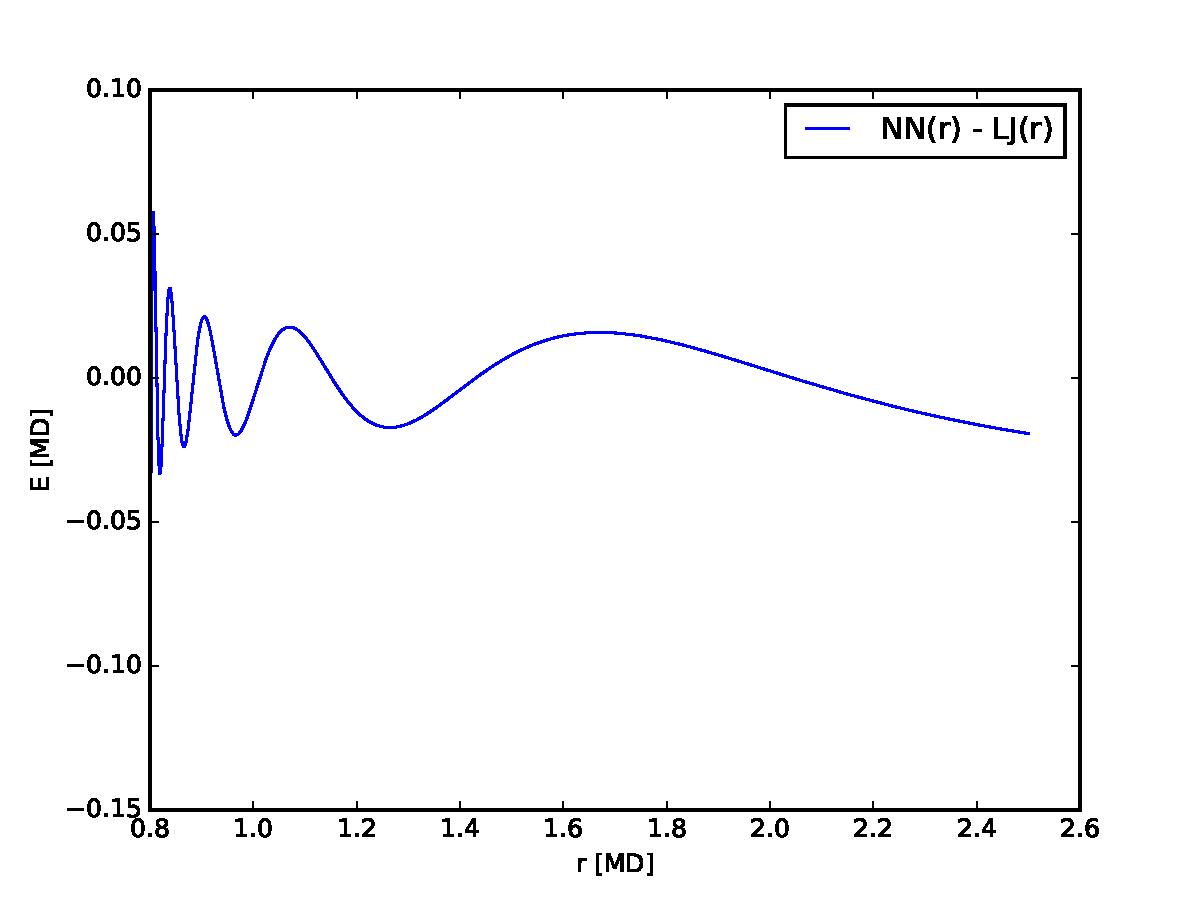
\includegraphics[width=\textwidth]{Figures/Tests/errorLJ.pdf}
\end{minipage}
\quad
\begin{minipage}[t]{0.48\linewidth}
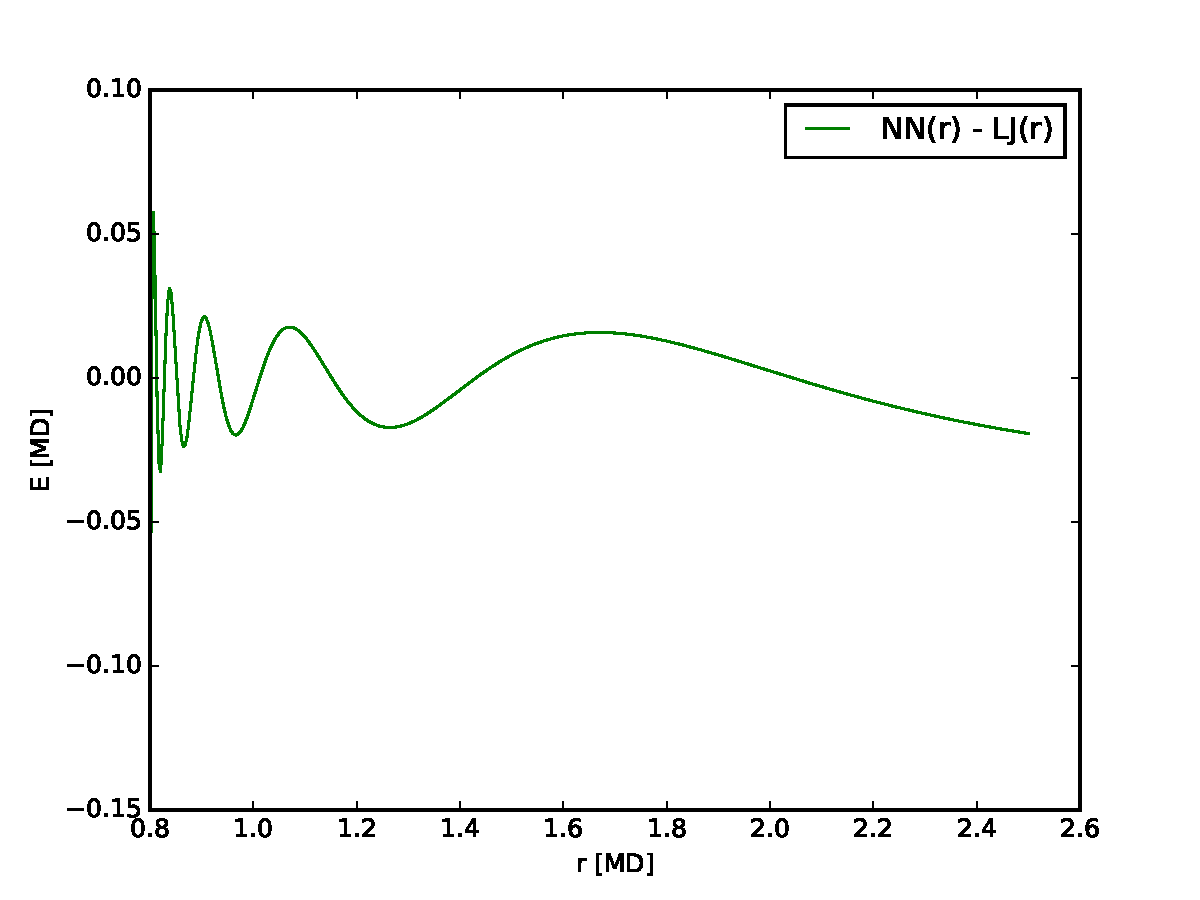
\includegraphics[width=\textwidth]{Figures/Tests/errorLJC.pdf}
\end{minipage}
  \caption{Error of a network trained to reproduce the shifted Lennard-Jones potential. 
           The NN is trained in Python and the error on the training data interval
           is calculated, shown on the left. The NN is also written to file for evaluation in C++, 
           shown on the right.}
\label{fig:errorLJTest}
\end{figure}
We observe that the error has excactly the same shape and value on the whole interval, we can therefore
confirm that the NN is implemented correctly. 

To test the implementation of the backpropagation algorithm, the
same NN is differentiated in C++ and compared to the analytical derivative of the L-J potential. 
The gradient of a NN is defined as the derivative of one of the outputs with respect to the input(s). 
There are two differences when using backpropagation to find the gradient of a network compared
to the use of backpropagation in training:
\begin{enumerate}
 \item The derivative of the output neuron's activation function is backpropagated instead of the output error
 \item We backpropagate all the way down to the input layer, during training we stop at the first hidden layer
\end{enumerate}
As mentioned before, the backpropagation algorithm is simply an application of the chain rule: 
To obtain the derivative of the output node with respect to the input nodes we need to differentiate through
all the nodes in-between because we have fully connected layers. The gradient error is plotted in 
\autoref{fig:errorBackPropTest}.
\begin{figure}[H]
\centering
  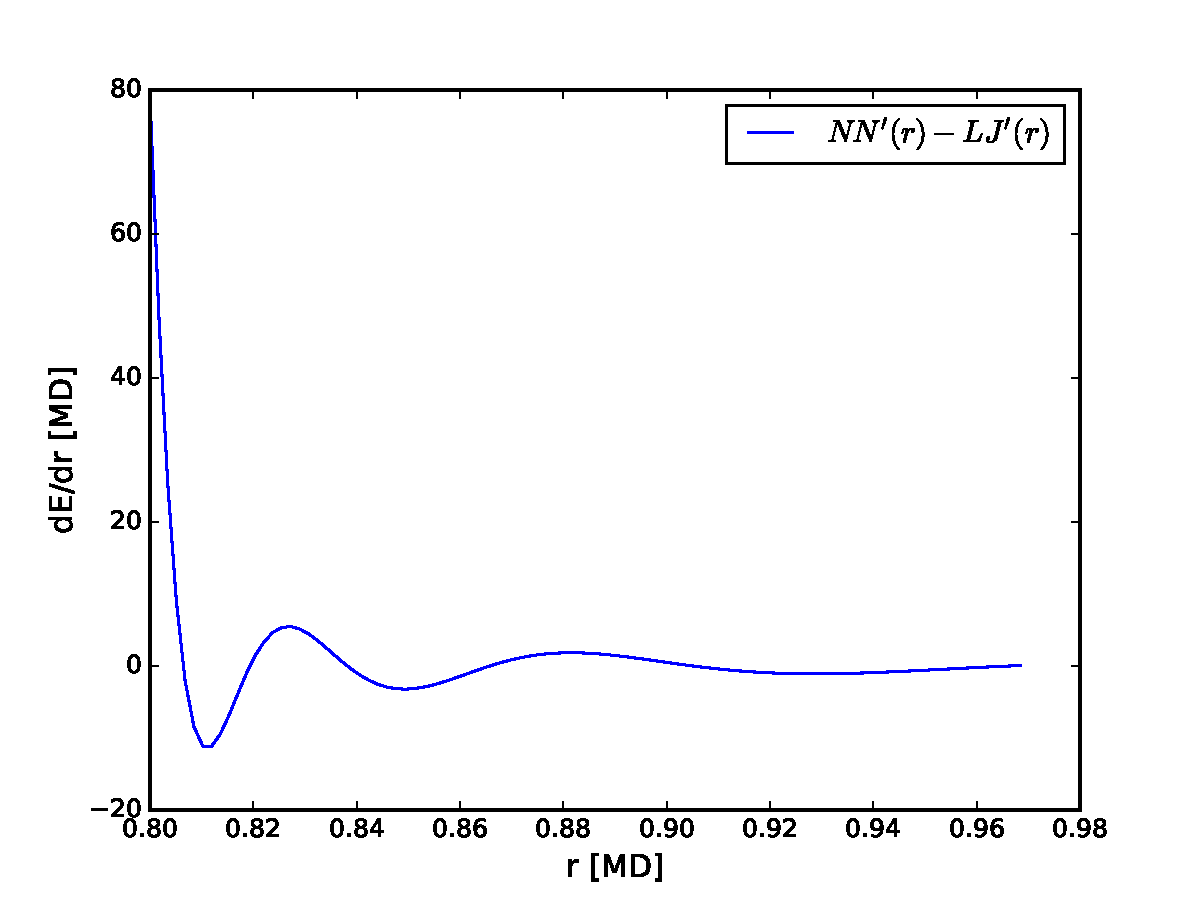
\includegraphics[width = 0.9\linewidth]{Figures/Tests/errorDerivative.pdf}
  \caption{Error of the gradient of a NN trained to reproduce the shifted Lennard-Jones potential.
	   The NN is trained in Python and evaluated and differentiated in C++ using the backpropagation algorithm.
	   The result is compared to the analytical derivative of the LJ potential. Only a part of the training
	   interval is shown, the graph is essentially flat after this point} 
  \label{fig:errorBackPropTest}
\end{figure}
Again we get an oscillating error over the training interval. The oscillations near the left end of the interval is much larger
than for the energy, but they get damped more quickly. The large error near the left end of the interval is a natural
consequence of the shape of the LJ potential for these values: the $1/r^{13}$ term dominates with its very steep slope, the NN is not 
fed a sufficient amount of data in this region to excactly reproduce the rapid changing derivative. 
This tells us that it is important to train the NN on a larger data interval than needed in simulations or possibly
feed the NN more data in critical regions during training. 

\subsection{Many-neighbour Lennard-Jones}
A NN can also be trained to obtain the energy of several neighbouring atoms at once. 
The training procedure is excactly the same, but now we train the network so that the output
is the sum of $N$ LJ-potentials for $N$ different distances $r$. The NN will have $N$ inputs and 1 output. 
To get an error of the same order as for 1 neighbour, we need to have a lot more nodes. The result of a training
session with $N=20$ inputs is shown in figures \autoref{fig:trainingManyNeighbourNN}. 
(Training session 02.12-19.36.50)
\begin{comment}
\begin{figure}[H]
\centering
  \begin{subfigure}[b]{0.75\textwidth}
  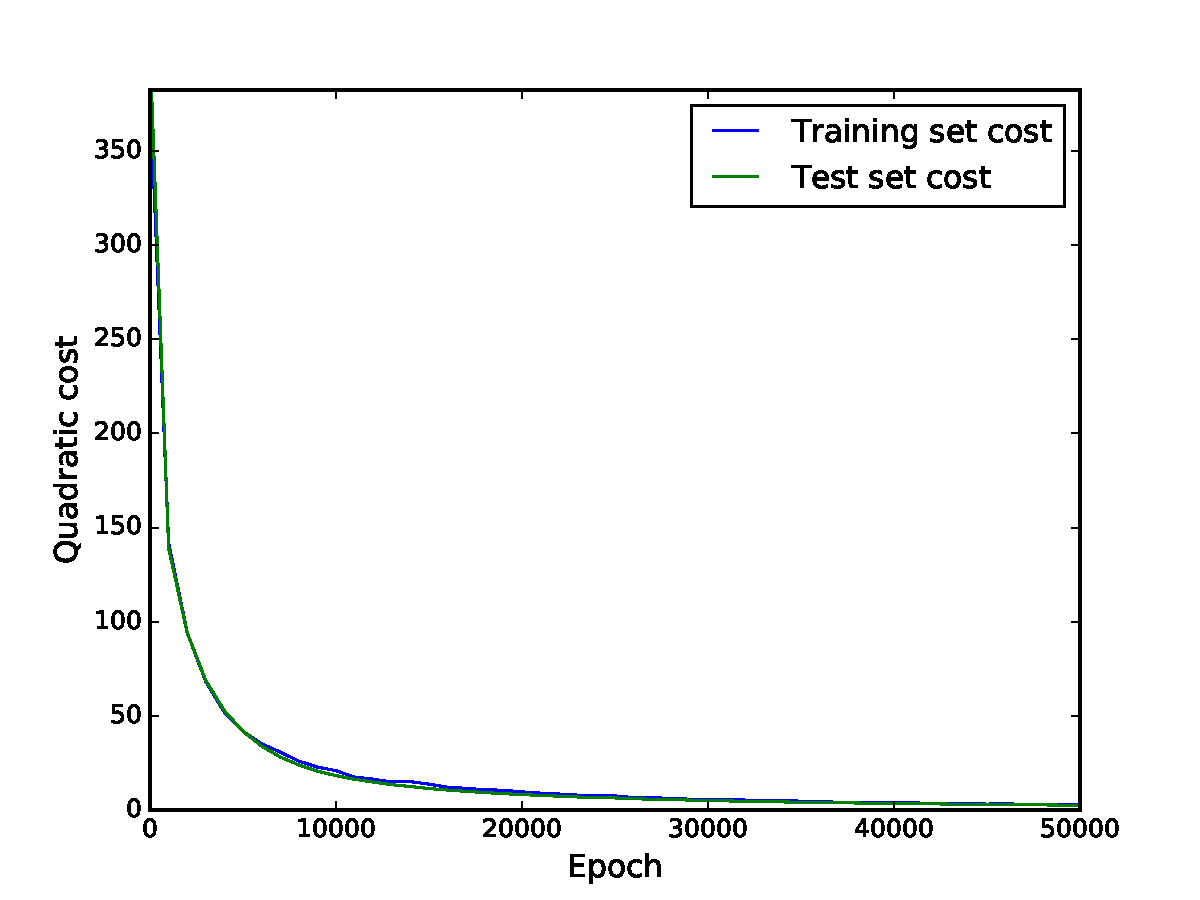
\includegraphics[width = 0.9\linewidth]{Figures/Tests/trainingManyNeighbourNN1.pdf}
\end{subfigure}
\begin{subfigure}
  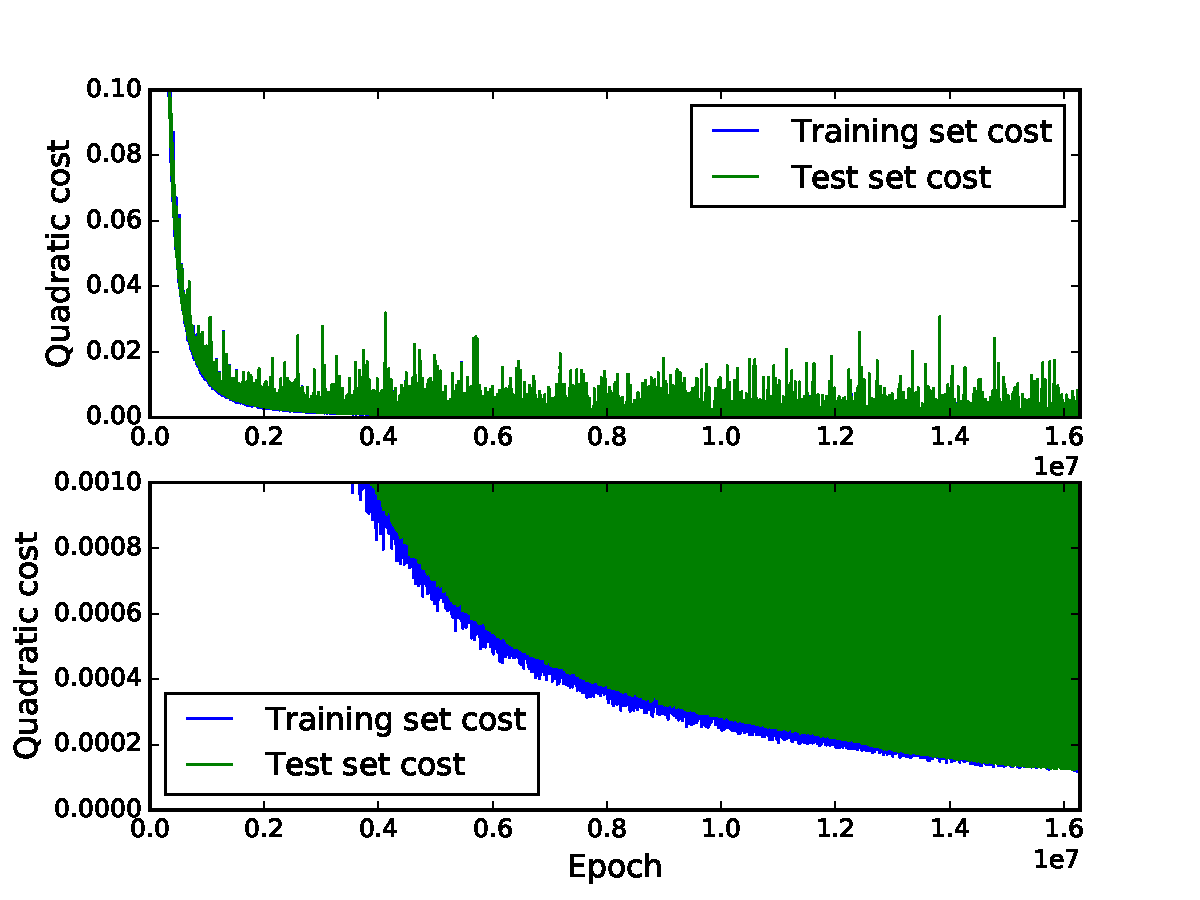
\includegraphics[width = 0.9\linewidth]{Figures/Tests/trainingManyNeighbourNN2.pdf}
  \end{subfigure}
  \label{fig:trainingManyNeighbourNN1}
  \caption{Error of the gradient of a NN trained to reproduce the shifted Lennard-Jones potential.
	   The NN is trained in Python and evaluated and differentiated in C++ using the backpropagation algorithm.
	   The result is compared to the analytical derivative of the LJ potential. Only a part of the training
	   interval is shown, the graph is essentially flat after this point} 
\end{figure}
\end{comment}
\begin{figure}[H]
\centering
\subcaptionbox{Zoomed out\label{zoomedOut}}{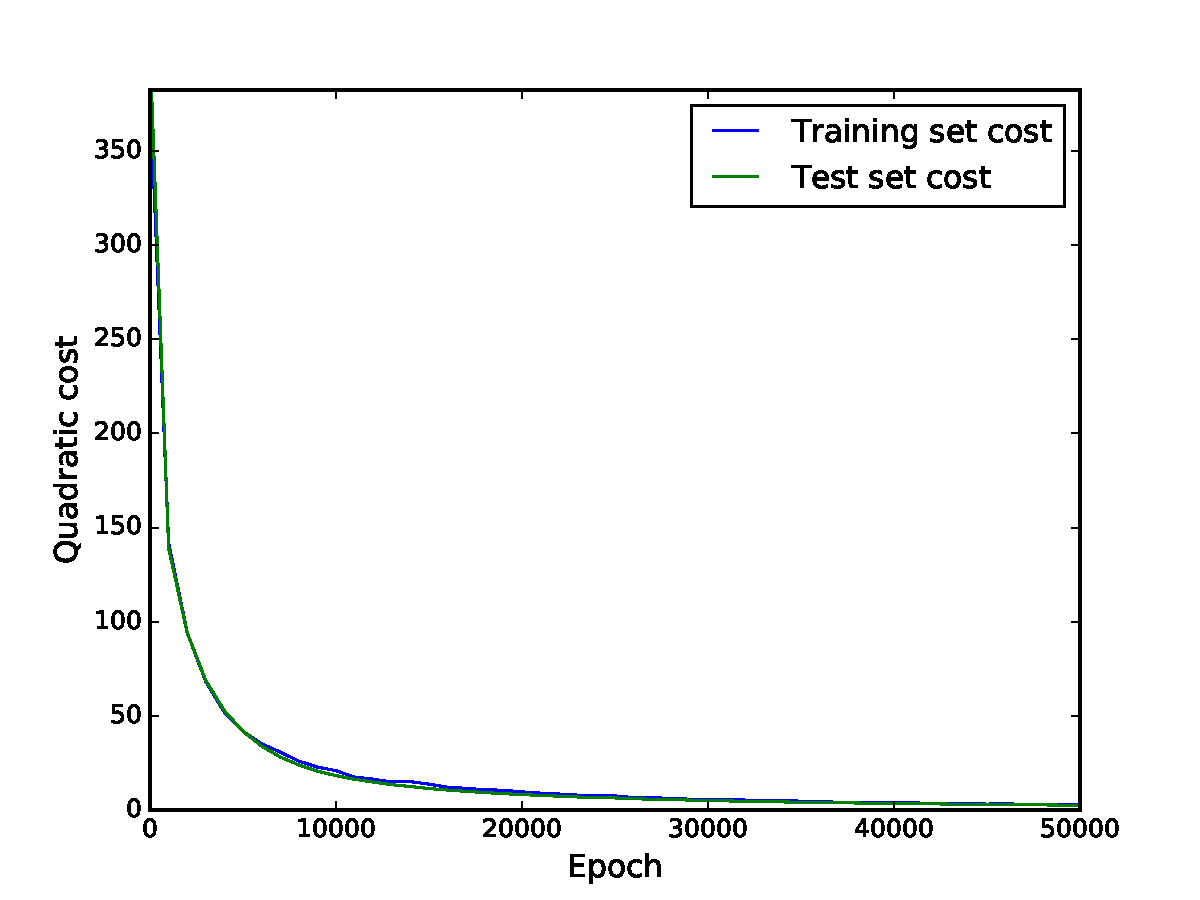
\includegraphics[width=0.8\textwidth]{Figures/Tests/trainingManyNeighbourNN1.pdf}
  }
\subcaptionbox{Zoomed in\label{zoomedIn}}{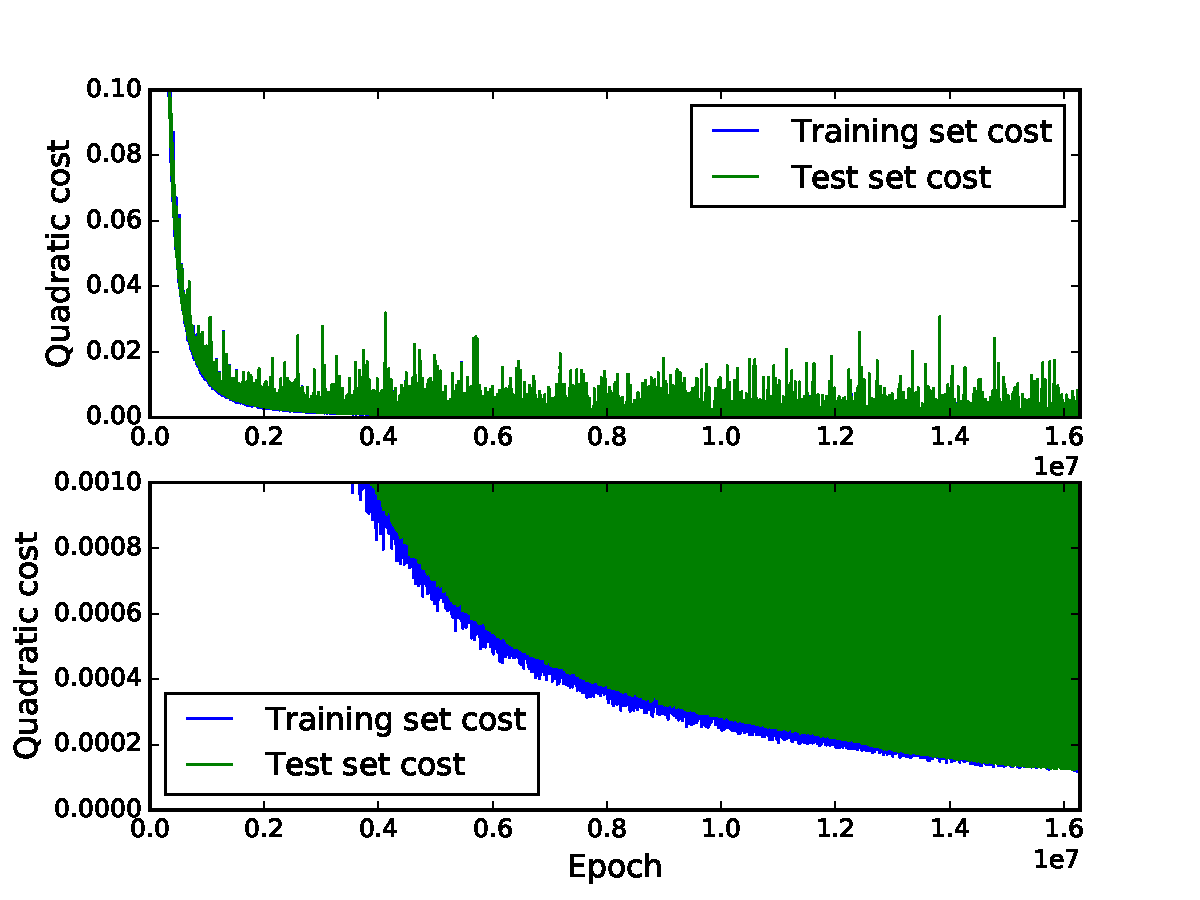
\includegraphics[width=0.8\textwidth]{Figures/Tests/trainingManyNeighbourNN2.pdf}}
\caption{Quadratic cost \eqref{quadraticCostFunction} of training set and test set for NN trained to yield
	 the sum of the shifted LJ-potential of 20 neighbouring atoms. 
	 The NN has 20 inputs, one hidden layer 
	 with 200 neurons and one output node. All nodes in the hidden layer have sigmoid activation functions 
	 \eqref{sigmoidActivationFunction}. \autoref{zoomedOut} shows the cost for the first 50 000 epochs, while
	 \autoref{zoomedIn} displays the cost for all epochs, but on a smaller scale.}	 
\label{fig:trainingManyNeighbourNN}
\end{figure}
The cost rapidly decreases during the first 10 000 epochs, then it starts to flatten out. This behaviour seems
to be general when doing regression with ANNs. 
There is no sign of overfitting: we do not observe an increase in the test cost relative to the training cost. 
This is (PROBABLY) due to the fact that our training set and test set are random numbers, i.e. there will be no 
specifics patterns or configurations present in the test set that is not covered by the training set. 
When we start doing training on data produced by MD trajectories or QM calculations, the situation will different.

The NN above outputs the total energy on an atom that is surrounded by $N$ neighbouring atoms, but it does not provide the forces. 
These must be obtained by calculating the analytical derivative of the NN with backpropagation as described above for each time step.
An alternative approach that may speed up the MD simulation is to have the NN also output the total force on the central atom. 
This can be done giving the cartesian coordinates and distance of N atoms as input to the NN so that each input
vector looks like
\begin{equation}
 (x_1, y_1, z_1, r_1, x_2, y_2, z_2, r_2, \dots, x_N, y_N, z_N, r_N)
\end{equation}
which yields an output vector
\begin{equation}
 (F_x^{TOT}, F_y^{TOT}, F_z^{TOT}, E^{TOT})
\end{equation}
We have to make sure that the input coordinates are in the range 
$x, y, z \in [-r_{cut}, r_{cut}]$ to cover the whole configuration space. The distances however, are still in the range
$r \in [a, r_{cut}]$ where $a$ is the minimum distance that two atoms can have in a given MD simulation (see function
\textit{energyAndForceCoordinates} in \textit{generateData}). As the NN now have 4 inputs per neighbour and 4 outputs, 
we need to have more nodes to get a sufficiently low error. We run a training session with 5 neighbours (20 inputs) 
(session 13.12-12.59.51). The cost has the same shape as before, but the error is much larger to begin with and also converges
slower (SKAL JEG GIDDE Å HA ENDA ET ERROR PLOT HER?).

One way to test if this works is to move only one of the input atoms while freezing the others and see if we reproduce
the LJ-potential form. We load the above training session and test with the command 
python approximateFunction2.py --load TrainingData/13.12-12.59.51/Checkpoints/ckpt-999 --test with this code: 
\begin{lstlisting}
if testFlag:
  
  # pick an input vector
  coordinates = xTrain[0]
  coordinates = coordinates.reshape([1,self.inputs])
  neighbours = self.inputs/4
  xNN = np.zeros(neighbours)
  yNN = np.zeros(neighbours)
  zNN = np.zeros(neighbours)
  rNN = np.zeros(neighbours)
  # extract coordinates and distances
  for i in range(neighbours):
      xNN[i] = coordinates[0,i*4]
      yNN[i] = coordinates[0,i*4 + 1]
      zNN[i] = coordinates[0,i*4 + 2]
      rNN[i] = coordinates[0,i*4 + 3]
		  
  # vary coordinates of only one atom and see 
  # if the resulting potential is similar to LJ
  N = 500
  r = np.linspace(0.8, 2.5, N)
  energyNN = []
  energyLJ = []
  forceNN = []
  forceLJ = []
  xyz = np.zeros(3)
  for i in range(N):
      r2 = r[i]**2
      xyz[0] = np.random.uniform(0, r2)
      xyz[1] = np.random.uniform(0, r2-xyz[0])
      xyz[2] = r2 - xyz[0] - xyz[1]
      #np.random.shuffle(xyz)
      x = np.sqrt(xyz[0])# * np.random.choice([-1,1])
      y = np.sqrt(xyz[1])# * np.random.choice([-1,1])
      z = np.sqrt(xyz[2])# * np.random.choice([-1,1])                      
      coordinates[0][0] = x; coordinates[0][1] = y; coordinates[0][2] = z
      coordinates[0][3] = r[i]
      energyAndForce = sess.run(prediction, feed_dict={self.x: coordinates})
      energyNN.append(energyAndForce[0][3]) 
      rNN[0] = r[i]
      energyLJ.append(np.sum(self.function(rNN)))
      forceNN.append(energyAndForce[0][0])
      xNN[0] = x
      forceLJ.append(np.sum(self.functionDerivative(rNN)*xNN/rNN))
  
  # convert to arrays
  energyNN = np.array(energyNN); energyLJ = np.array(energyLJ)
  forceNN = np.array(forceNN); forceLJ = np.array(forceLJ)
  
  # plot error 
  plt.plot(r, energyNN - energyLJ)
  plt.show()
  plt.plot(r, forceNN - forceLJ)
  plt.show()
  print 'Cost: ', (np.sum((energyNN - energyLJ)**2 + (forceNN - forceLJ)**2))/N
  
  # see if the energy is zero when all neighbours is at cutoff distance
  inputz = np.array([1.87, 1.32, 1.006, 2.5]*neighbours).reshape([1,self.inputs])
  r = np.array([2.5]*neighbours)
  energyLJ = sum(self.function(r))               
  ef = sess.run(prediction, feed_dict={self.x: inputz})
  
  print 'Approximate energy: ', ef[0,3]
  print 'LJ energy: ', energyLJ
  
  numberOfEpochs = 0
\end{lstlisting}
which produces the following output: 
\begin{lstlisting}
Model restored
Cost:  0.132622806039
NN energy at cutoff:  0.125104
LJ energy at cutoff:  0.0
Time elapsed: 1.2e-05
\end{lstlisting}
We see that the NN energy at cutoff is not zero, because of the cost (IS THIS CORRECT? THE COST AT CUTOFF IS PRACTICALLY ZERO).
The error of the NN energy and forces over the training data interval is shown in 
\begin{figure}[H]
\begin{minipage}[t]{0.48\linewidth}
  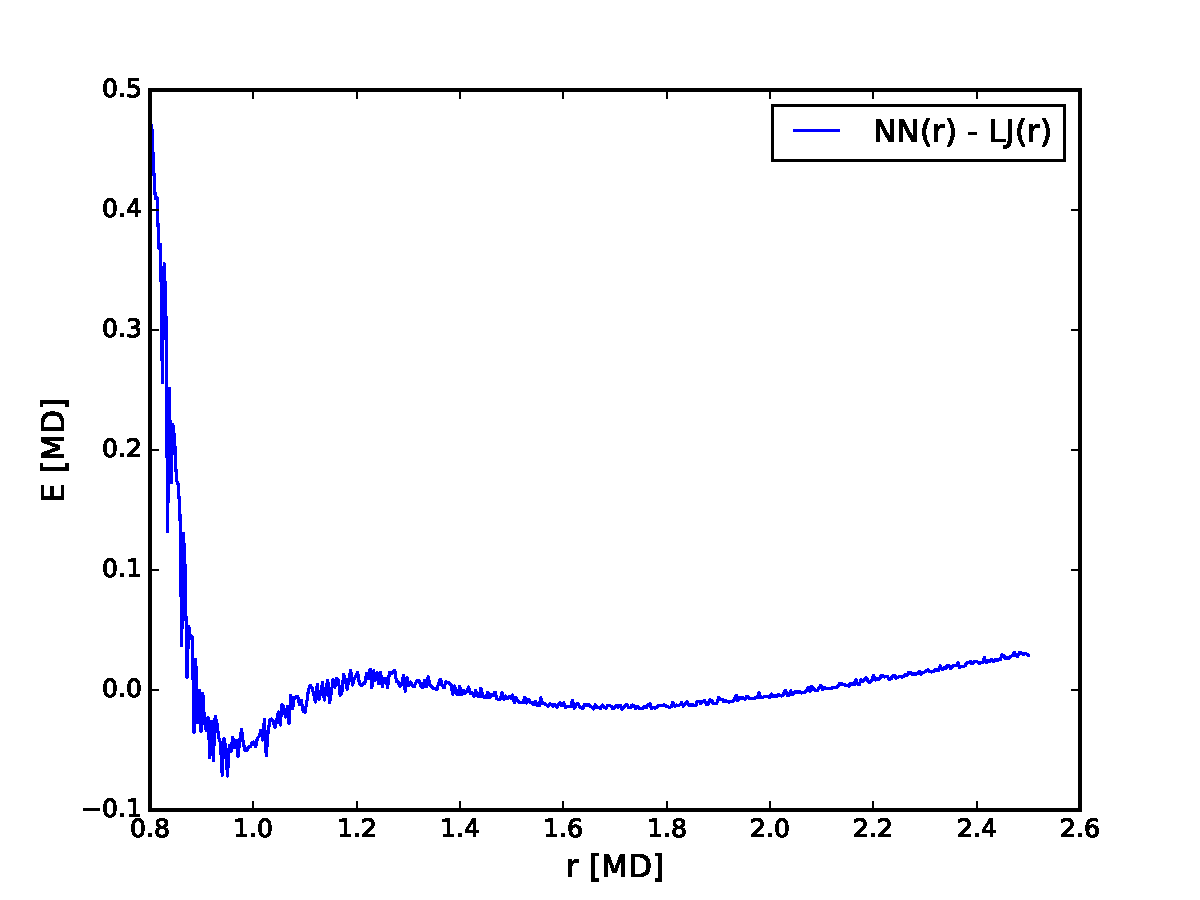
\includegraphics[width=\textwidth]{Figures/Tests/manyNeighbourEnergyError.pdf}
\end{minipage}
\quad
\begin{minipage}[t]{0.48\linewidth}
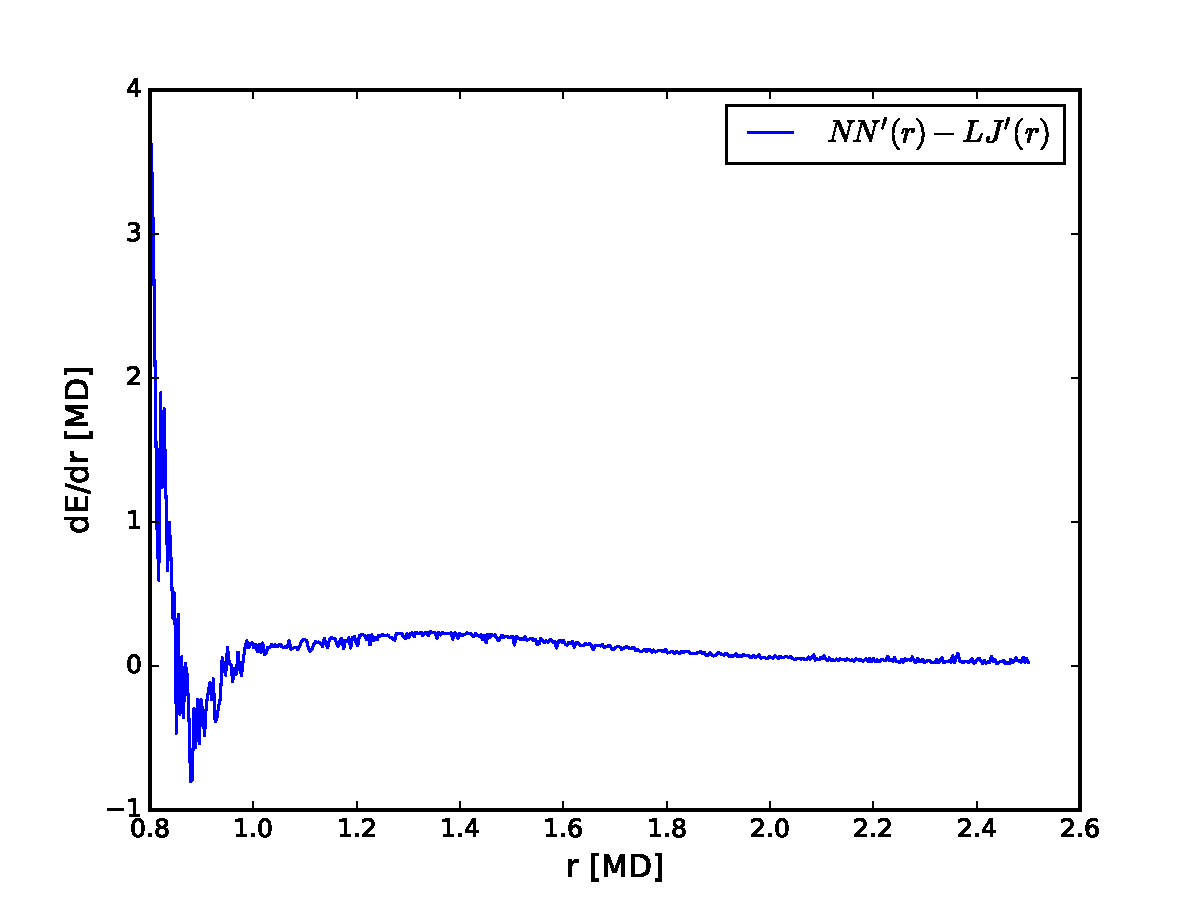
\includegraphics[width=\textwidth]{Figures/Tests/manyNeighbourForceError.pdf}
\end{minipage}
  \caption{Error of a network trained to yield the total energy and force on a central atom from 5 neighbouring atoms. 
           The energy contribution from each neighbour is a shifted LJ potential. Trained for 1e6 epochs, 100 nodes
           in 2 layers. The energy error is shown on the left, force error on the right.}
\label{fig:errorManyNeighbourNN}
\end{figure}
The error oscillates in exactly the same way as for the 1-input NN above, suggesting that the training is done correctly. 
However, it is very important that the energies and forces in an MD simulation is consistent, and this is not 
ensured here, where the two are obtained in a somewhat independent way. Any incosistency between the energies and forces
will magnify for each time step, resulting in inaccurate statistical properties like temperature and pressure. 
Therefore it is a better idea to have the NN only output the total energy, and find the forces by analytically
differentiating the NN for each time step. $\SI{4}{\angstrom}$

\part{Results and discussion}

\chapter{NN potential for Si} \label{sec:SiPotentialResults}
Construct an NN potential for Si that works in a certain temperature range (only solid, or liquid too?)
Compute thermodynamic properties and things like radial distrubution function and compare both 
with experiments and with results with Stillinger-Weber. 

\chapter{NN potential for SiO2}
Construct an NN potential for SiO2 that works in a certain temperature range (only solid, or liquid too?). 
Can use various potentials as the black box, e.g. Vashishta or ReaxFF. 
ReaxFF would be great, because then we would maybe get a speed-up. 


\begin{appendices}

\chapter{Symmetry functions derivatives} \label{app:appendixA1}
We list here the derivatives of the symmetry functions used for training neural networks. These have to be known
to compute forces for MD simulations. In some cases we only show the deriviative with respect to 
$R = \sqrt{x^2 + y^2 + z^2}$. 
Each component $\alpha$ can be calculated by
\begin{equation}
 \frac{\partial R}{\partial \alpha} = \frac{\alpha}{R}
\end{equation}
The following notation applies in the following,
\begin{equation}
 R_{ij} = \Bigr(x_{ij}^2 + y_{ij}^2 + z_{ij}^2\Bigr)^{1/2} =
 \Bigr((x_j - x_i)^2 + (y_j - y_i)^2 + (z_j - z_i)^2\Bigr)^{1/2}
\end{equation}
Cutoff function \eqref{cutoffFunction}:
\begin{equation}
 \frac{\partial f_c(R)}{\partial R} = -\frac{1}{2}\frac{\pi}{R_c} \sin\left(\frac{\pi R}{R_c}\right) = M(R)
 \label{cutOffFunctionDerivative}
\end{equation}
This expression is valid for all combinations of indicies. The derivatives w.r.t. to individual coordinates are
\begin{equation}
 \frac{\partial f_c(R_{ij})}{\partial x_{ij}} = M(R_{ij})
 \frac{x_{ij}}{R_{ij}}
 \label{cutOffFunctionDerivative1}
\end{equation}
and 
\begin{equation}
 \frac{\partial f_c(R_{ik})}{\partial x_{ik}} = M(R_{ik})
 \frac{x_{ik}}{R_{ik}}
 \label{cutOffFunctionDerivative1}
\end{equation}
while
\begin{equation}
 \frac{\partial f_c(R_{ij})}{\partial x_{ik}} = \frac{\partial f_c(R_{ik})}{\partial x_{ij}} = 0
\end{equation}
because atom $i$ is always in origo, which means we can do the substitutions $x_{ij} \rightarrow x_{j}$ and 
$x_{ik} \rightarrow x_{k}$. SHOULD I DO THIS CONSEQUENTLY BELOW????. Also, 
\begin{equation}
 \frac{\partial f_c(R_{jk})}{\partial x_{ij}} = -M(R_{jk})
 \frac{x_{jk}}{R_{jk}}
 \label{cutOffFunctionDerivative1}
\end{equation}
and 
\begin{equation}
 \frac{\partial f_c(R_{jk})}{\partial x_{ij}} = M(R_{jk})
 \frac{x_{jk}}{R_{jk}}
 \label{cutOffFunctionDerivative1}
\end{equation}
The derivative of each term in $G_i^1$ \eqref{G1} is simply \eqref{cutOffFunctionDerivative}. \\
$G_i^2$ \eqref{G2}:
\begin{equation}
 \frac{\partial G_i^2}{R_{ij}} = 
 \exp(-\eta(R_{ij}-R_s)^2) \left[2\eta(R_s - R_{ij}) + \frac{\partial f_c}{\partial R_{ij}}\right]
\end{equation}
$G_i^3$ has not been used in this theses. \\
$G_i^4$ \eqref{G4}:
\begin{equation}
 G_i^4 = F_1(\theta)F_2(R_{ij},R_{ik},R_{jk})F_3(R_{ij},R_{ij},R_{jk})
\end{equation}
where
\begin{align}
 F_1(\theta) &= 2^{1-\zeta}(1 + \lambda \cos\theta_{ijk})^\zeta \\
 F_2(R_{ij},R_{ik},R_{jk}) &= \exp[-\eta (R_{ij}^2 + R_{ik}^2 + R_{jk}^2)] \\
 F_3(R_{ij},R_{ij},R_{jk}) &= f_c(R_{ij}) f_c(R_{ik}) f_c (R_{jk})
\end{align}
where
\begin{equation}
 \cos\theta = \frac{x_{ij}x_{ik} + y_{ij}y_{ik} + z_{ij}z_{ik}}{R_{ij}R_{ik}}
\end{equation}
Using the product rule:
\begin{align}
 \frac{\partial G_i^4}{\partial x_{ij}} = &\frac{\partial F_1}{x_{ij}} F_2 F_3 + 
 F_1 \left(\frac{\partial F_2}{\partial x_{ij}}F_3 + F_2\frac{\partial F_3}{\partial x_{ij}}\right) \\
 &\frac{\partial F_1}{x_{ij}} F_2 F_3 + 
 F_1 \frac{\partial F_2}{\partial x_{ij}}F_3 + F_1F_2\frac{\partial F_3}{\partial x_{ij}}
 \label{G4Derivative}
\end{align}
We have
\begin{equation}
 \frac{\partial F_1}{\partial x_{ij}} = \frac{\partial F_1}{\partial\cos\theta}
 \frac{\partial\cos\theta}{\partial x_{ij}}
\end{equation}
where
\begin{equation}
 \frac{\partial F_1}{\partial\cos\theta} = \lambda\zeta(1 + \cos\theta)^{\zeta-1} = K
\end{equation}
and 
\begin{equation}
 \frac{\partial\cos\theta}{\partial x_{ij}} = \frac{x_{ik}}{r_{ij}r_{ik}} - 
 \frac{x_{ij}\cos\theta}{r_{ij}^2}
\end{equation}
To get the corresponding expression for $x_{ik}$, simply substitute $x_{ij} \leftrightarrow x_{ik}$ and 
$r_{ij} \leftrightarrow r_{ik}$. Further, 
\begin{align}
 \frac{\partial F_2}{\partial x_{ij}} &= \frac{\partial F_2}{\partial r_{ij}}\frac{\partial r_{ij}}{\partial x_{ij}}  = 
 (-2\eta r_{ij}\frac{x_{ij}}{r_{ij}} - 2\eta r_{jk}\frac{x_{jk}}{r_{jk}})\exp[-\eta (R_{ij}^2 + R_{ik}^2 + R_{jk}^2)] \\
 &= -2\eta F_2 x_{ij} - 2\eta F_2 x_{jk}
\end{align}
The corresponding expression for $x_{ik}$ is
\begin{equation}
 \frac{\partial F_2}{\partial x_{ik}} = 
 -2\eta F_2 x_{ik} + 2\eta F_2 x_{jk}
\end{equation}
Lastly, 
\begin{align}
 \frac{\partial F_3}{\partial x_{ij}} &=  \frac{\partial f_c(r_{ij})}{\partial x_{ij}}
 f_c(r_{ik}) f_c(r_{jk}) + f_c(r_{ij})f_c(r_{ik})\frac{\partial f_c(r_{jk})}{\partial x_{ij}} \\
 &= f_c(r_{ik})\Biggr(M(r_{ij})\frac{x_{ij}}{r_{ij}}f_c(r_{jk}) - 
 f_c(r_{ij}) M(r_{jk})\frac{x_{jk}}{r_{jk}} \Biggr)
\end{align}
The corresponding expression for $x_{ik}$ is
\begin{align}
 \frac{\partial F_3}{\partial x_{ik}} &= f_c(r_{ij})\Biggr(\frac{\partial f_c(r_{ik})}{\partial x_{ik}}f_c(r_{jk}) + 
 f_c(r_{ik}) \frac{\partial f_c(r_{jk})}{\partial x_{ik}} \Biggr) \\
 &= f_c(r_{ij})\Biggr(M(r_{ik})\frac{x_{ik}}{r_{ik}}f_c(r_{jk}) + 
 f_c(r_{ik}) M(r_{jk})\frac{x_{jk}}{r_{jk}} \Biggr) \\
\end{align}
Then, taking \eqref{G4Derivative} into account:
\begin{align}
 \frac{\partial G_i^4}{\partial x_{ij}} = &\biggr(\frac{x_{ik}}{r_{ij}r_{ik}} - \frac{x_{ij}\cos\theta}{r_{ij}^2}
 \biggr)KF_2F_3 \, - \\ &2\eta F_1F_2F_3 x_{jk} - 2\eta F_1F_2F_3 x_{ij} \, + \\
 &F_1F_2 f_c(r_{ik})\Biggr(M(r_{ij})\frac{x_{ij}}{r_{ij}}f_c(r_{jk}) +
 f_c(r_{ij}) M(r_{jk})\frac{x_{jk}}{r_{jk}} \Biggr)
\end{align}
and for $x_{ik}$:
\begin{align}
 \frac{\partial G_i^4}{\partial x_{ik}} = &\biggr(\frac{x_{ij}}{r_{ij}r_{ik}} - \frac{x_{ik}\cos\theta}{r_{ik}^2}
 \biggr)KF_2F_3 \, + \\ &2\eta F_1F_2F_3 x_{jk} - 2\eta F_1F_2F_3 x_{ik} \, + \\
 &F_1F_2 f_c(r_{ij})\Biggr(M(r_{ik})\frac{x_{ik}}{r_{ik}}f_c(r_{jk}) - 
 f_c(r_{ik}) M(r_{jk})\frac{x_{jk}}{r_{jk}} \Biggr)
\end{align}
or in terms of $x_{ij}$ and $x_{ik}$ and $x_{jk}$:
\begin{align}
 \frac{\partial G_i^4}{\partial x_{ij}} = &x_{ij} \biggr(-\frac{\cos\theta}{r_{ij}^2}K
 F_2F_3 - 2\eta F_1F_2F_3 \, + \\ 
 &F_1F_2M(r_{ij})f_c(r_{ik})f_c(r_{jk})\frac{1}{r_{ij}}\biggr) \, + \\
 &x_{ik}\frac{KF_2F_3}{r_{ij}r_{ik}} - x_{jk}\Bigr(F_1F_2M(r_{jk})f_c(r_{ik})f_c(r_{ij}) + 2\eta F_1F_2F_3\Bigr)\frac{1}{r_{jk}}
\end{align}
and 
\begin{align}
 \frac{\partial G_i^4}{\partial x_{ik}} = &\frac{x_{ik}}{r_{ik}} \biggr(-\frac{\cos\theta}{r_{ik}^2}K
 F_2F_3 - 2\eta F_1F_2F_3 \, + \, \\
 &F_1F_2M(r_{ik})f_c(r_{ij})f_c(r_{jk})\frac{1}{r_{ik}}\biggr) + \, \\
 &x_{ij}\frac{KF_2F_3}{r_{ij}r_{ik}} + x_{jk}\Bigr(F_1F_2M(r_{jk})f_c(r_{ij})f_c(r_{ik}) - 2\eta F_1F_2F_3\Bigr)\frac{1}{r_{jk}}
\end{align}
The derivative of $G_i^5$ \eqref{G5} is found in a similar way,
\begin{equation}
 G_i^5 = F_1(\theta)F_2(R_{ij},R_{ik})F_3(R_{ij},R_{ij})
\end{equation}
where 
\begin{align}
 F_1(\theta) &= 2^{1-\zeta}(1 + \lambda \cos\theta_{ijk})^\zeta \\
 F_2(R_{ij},R_{ik}) &= \exp[-\eta (R_{ij}^2 + R_{ik}^2)] \\
 F_3(R_{ij},R_{ij}) &= f_c(R_{ij}) f_c(R_{ik})
\end{align}
The derivative of $F_1$ is the same, while for $F_2$ we obtain
\begin{equation}
 \frac{\partial F_2}{\partial x_{ij}} = -2\eta F_2 x_{ij}
\end{equation}
and
\begin{equation}
 \frac{\partial F_2}{\partial x_{ik}} = -2\eta F_2 x_{ik}
\end{equation}
For $F_3$, 
\begin{equation}
 \frac{\partial F_3}{\partial x_{ij}} = \frac{\partial f_c(r_{ij})}{\partial x_{ij}}\frac{x_{ij}}{r_{ij}}
 f_c(r_{ik}) = M(r_{ij})f_c(r_{ik})\frac{x_{ij}}{r_{ij}}
\end{equation}
and
\begin{equation}
  \frac{\partial F_3}{\partial x_{ik}} = f_c(r_{ij})
 \frac{\partial f_c(r_{ik})}{\partial x_{ij}}\frac{x_{ik}}{r_{ik}} = 
 f_c(r_{ij})M(r_{ik})\frac{x_{ik}}{r_{ik}}
\end{equation}
so that
\begin{align}
 \frac{\partial G_i^5}{\partial x_{ij}} = &\biggr(\frac{x_{ik}}{r_{ij}r_{ik}} - \frac{x_{ij}\cos\theta}{r_{ij}^2}
 \biggr)KF_2F_3 -
 2\eta F_1 F_2F_3 x_{ij} \, + \\
 &F_1F_2 M(r_{ij})f_c(r_{ik})\frac{x_{ij}}{r_{ij}}
\end{align}
and 
\begin{align}
 \frac{\partial G_i^5}{\partial x_{ik}} = &\biggr(\frac{x_{ij}}{r_{ij}r_{ik}} - \frac{x_{ij}\cos\theta}{r_{ik}^2}
 \biggr)KF_2F_3 -
 2\eta F_1 F_2F_3 x_{ik} \, + \\
 &F_1F_2 M(r_{ik})f_c(r_{ij})\frac{x_{ik}}{r_{ik}}
\end{align}
In terms of $x_{ij}$ and $x_{ik}$:
\begin{align}
 \frac{\partial G_i^5}{\partial x_{ij}} = \, &x_{ij} \biggr(-\frac{\cos\theta}{r_{ij}^2}K
 F_2F_3 - 2\eta F_1F_2F_3 + F_1F_2M(r_{ij})f_c(r_{ik})\frac{1}{r_{ij}} \biggr) \, + \\
 &x_{ik}\frac{KF_2F_3}{r_{ij}r_{ik}}
\end{align}
and 
\begin{align}
 \frac{\partial G_i^5}{\partial x_{ik}} = \, &x_{ik} \biggr(-\frac{\cos\theta}{r_{ik}^2}K
 F_2F_3 - 2\eta F_1F_2F_3 + F_1F_2M(r_{ik})f_c(r_{ij})\frac{1}{r_{ik}} \biggr) \, + \\
 &x_{ij}\frac{KF_2F_3}{r_{ij}r_{ik}}
\end{align}


\end{appendices}





\newpage

\begin{thebibliography}{56}

\bibitem{Behler11general}
 J. Behler.
 ''Neural network potential-energy surfaces in chemistry: a tool for large-scale simulations''.
 In: \textit{Phys. Chem. Chem. Phys.} 13. (2011), 17930-17955. 
 DOI: \href{http://dx.doi.org/10.1039/c1cp21668f}{10.1039/c1cp21668f}. 
 
\bibitem{Behler11symmetry}
 J. Behler.
 ''Atom-centered symmetry functions for constructing high-dimensional neural network potentials''.
 In: \textit{The Journal of Chemical Physics} 134. (2011), 074106. 
 DOI: \href{http://dx.doi.org/10.1063/1.3553717}{10.1063/1.3553717}.
 
\bibitem{Dragly14}
 S. A. Dragly.
 ''Bridging quantum mechanics and molecular dynamics with artificial neural networks''.
 MA thesis. University of Oslo (2014). \\
 URL: \href{https://www.duo.uio.no/handle/10852/41843}{https://www.duo.uio.no/handle/10852/41843}.

\bibitem{Hornik89}
 K. Hornik, M. Stinchcombe, and H. White.
 ''Multilayer Feedforward Networks are Universal Approximators''.
 In: \textit{Neural Networks} 2. (1989), 359. 
 DOI: \href{https://doi.org/10.1016/0893-6080(89)90020-8}{10.1016/0893-6080(89)90020-8}
 
\bibitem{Rojas96}
 R. Rojas. 
 \textit{Neural Networks: A Systematic Introduction}.
 Springer, 1996.
 
\bibitem{Karlik11}
 B. Karlik and A. V. Olgac.
 ''Performance Analysis of Various Activation Functions in Generalized MLP Architectures of Neural Networks''.
 In: \textit{IJAE} 1. (2011), 111-122.
 
\bibitem{LeCun15}
 Y. LeCun, Y. Bengio, and G. Hinton.
 ''Deep learning''.
 In: \textit{Nature} 521. (2015), 436-444. 
 DOI: \href{http://dx.doi.org/10.1038/nature14539}{10.1038/nature14539}
 
\bibitem{Glorot11}
 X. Glorot, A. Bordes, and Y. Bengio.
 ''Deep Sparse Rectifier Neural Networks''.
 In: \textit{JMLR} 15. (2011), 315-323.
 
\bibitem{Rumelhart86}
 D. E. Rumelhart, G. E. Hinton, and R. J. Williams.
 ''Learning representations by back-propagating errors''.
 In: \textit{Nature} 323. (1986), 533-536.
 DOI: \href{http://dx.doi.org/10.1038/323533a0}{10.1038/323533a0}
 
\bibitem{Behler15}
 J. Behler.
 ''Constructing High-Dimensional Neural Network Potentials: A Tutorial Review''.
 In: \textit{International Journal of Quantum Chemistry} 115. (2015), 1032-1050.
 DOI: \href{http://dx.doi.org/10.1002/qua.24890}{10.1002/qua.24890}
 
\bibitem{Tuckerman92}
 Tuckerman, Berne, and Martyna .
 ''Reversible multiscale molecular dynamics''.
 In: \textit{J. Chem. Phys.} 97. (1992), 1990.
 
\bibitem{Plimpton95}
 S. Plimpton. 
 ''Fast Parallel Algorithms for Short-Range Molecular Dynamics''.
 In: \textit{Journal of Computational Physics} 117. (1995) 1-19. 
 DOI: \href{https://doi.org/10.1006/jcph.1995.1039}{10.1006/jcph.1995.1039}. 
 
\bibitem{Abadi15}
 M. Abadi, A. Agarwal, P. Barham, E. Brevdo,
 Z. Chen, C. Citro, G. S. Corrado, A. Davis,
 J. Dean, M. Devin, S. Ghemawat, I. Goodfellow,
 A. Harp, G. Irving, M. Isard, R. Jozefowicz, Y. Jia,
 L. Kaiser, M. Kudlur, J. Levenberg, D. Mané, M. Schuster,
 R. Monga, S. Moore, D. Murray, C. Olah, J. Shlens,
 B. Steiner, I. Sutskever, K. Talwar, P. Tucker,
 V. Vanhoucke, V. Vasudevan, F. Viégas,
 O. Vinyals, P. Warden, M. Wattenberg, M. Wicke,
 Y. Yu and X. Zheng.
 ''TensorFlow: Large-scale machine learning on heterogeneous systems''.
 \textit{Google Research} (2015). 
 arXiv: \href{https://arxiv.org/abs/1603.04467}{1603.04467}
 
\bibitem{Abadi16}
 M. Abadi, P. Barham, J. Chen, Z. Chen, A. Davis, J. Dean,
 M. Devin, S. Ghemawat, G. Irving, M. Isard, M. Kudlur,
 J. Levenberg, R. Monga, S. Moore, D. G. Murray, B. Steiner, P. Tucker,
 V. Vasudevan, P. Warden, M. Wicke, Y. Yu, and X. Zheng.
 ''TensorFlow: A System for Large-Scale Machine Learning''.
 \textit{Google Brain} (2016).
 arXiv: \href{https://arxiv.org/abs/1605.08695}{1605.08695}
 
\bibitem{Qian99}
 N. Qian.
 ''On the momentum term in gradient descent learning algorithms''
 In: \textit{Neural Networks} 12(1). (1999) 145-151. 
 DOI: \href{https://doi.org/10.1016/S0893-6080(98)00116-6}{10.1016/S0893-6080(98)00116-6}
 
\bibitem{Duchi11}
 J. Duchi, E. Hazan, and Y. Singer.
 ''Adaptive Subgradient Methods for Online Learning and Stochastic Optimization''.
 In \textit{The Journal of Machine Learning Research} 12. (2011) 2121-2159. 
 URL: \href{http://jmlr.org/papers/v12/duchi11a.html}{http://jmlr.org/papers/v12/duchi11a.html}
 
\bibitem{Zeiler12}
 M. D. Zeiler. 
 ''Adadelta: an adaptive learning rate method''. (2012).
 arXiv: \href{https://arxiv.org/abs/1212.5701}{1212.5701}
 
\bibitem{Kingma14}
 D. P. Kingma and J. Ba.
 ''Adam: A Method for Stochastic Optimization''. (2014).
 arXiv: \href{https://arxiv.org/abs/1412.6980}{1412.6980}
 
\bibitem{Ischtwan94}
 J. Ischtwan and M. A. Collins.
 ''Molecular potential energy surfaces by interpolation''.
 In: \textit{The Journal of Chemical Physics} 100. (1994), 8080.
 DOI: \href{http://dx.doi.org/10.1063/1.466801}{10.1063/1.466801}
 
\bibitem{Raff05}
 L. M. Raff, M. Malshe, M. Hagan, D. I. Doughan, M. G. Rockley, and R. Komanduri.
 ''Ab inito potential-energy surfaces for complex, multichannel systems using modified
 novelty sampling and feedforward neural networks''. 
 In: \textit{The Journal of Chemical Physics} 122. (2005), 084104. 
 DOI: \href{http://dx.doi.org/10.1063/1.1850458}{10.1063/1.1850458}
 
\bibitem{Raff12}
 L. M. Raff, R. Komanduri, M. Hagan, and S. T. S. Bukkapatnam 
 \textit{Neural networks in chemical reaction dynamics}.
 Oxford University Press, 2012.
 
\bibitem{Pukrittayakamee09}
 A. Pukrittayakamee, M. Malshe, M. Hagan, L. M. Raff, and R. Narulkar, 
 S. Bukkapatnum and R. Komanduri. 
 ''Simultaneous fitting of a potential-energy surface and its corresponding force fields
 using feedforward neural networks''. 
 In: \textit{The Journal of Chemical Physics} 130. (2009) 134101.
 DOI: \href{http://dx.doi.org/10.1063/1.3095491}{10.1063/1.3095491}
 
\bibitem{McCulloch43}
 W. S. McCulloch and W. Pitts.
 ''A logical calculus of the ideas immanent in nervous activity''.
 In: \textit{Bulletin of Mathematical Biophysics} 5. (1943), 115. 
 DOI: \href{http://dx.doi.org/10.1007/BF02478259}{10.1007/BF02478259}
 
\bibitem{Kriesel07}
 D. Kriesel. 
 ''A Breif Introduction to Neural Networks''
 Available at \href{http://www.dkriesel.com}{http://www.dkriesel.com}
 
\bibitem{LeCun99}
 Y. LeCun, P. Haffner, L. Bottou, and Y. Bengio. 
 ''Object recognition with Gradient-Based Learning''.
 In: \textit{Shape, Contour and Grouping in Computer Vision. Lecture Notes in Computer Science}.
 1681. (1999) 319-345. 
 DOI: \href{http://dx.doi.org/10.1007/3-540-46805-6_19}{10.1007/3-540-46805-6\_19}
 
\bibitem{Rosenblatt58}
 F. Rosenblatt. 
 ''The Perceptron: A probabilistic model for information storage and organization in the brain.''
 In: \textit{Psychological Review} 65. (1958), 386-408. 
 
\bibitem{Ruder16}
 S. Ruder.
 ''An overview of gradient descent optimization algorithms.''
 (2016). 
 arXiv: \href{https://arxiv.org/abs/1609.04747}{1609.04747}
 
\bibitem{Dawes08}
 R. Dawes, D. L. Thompson, A. F. Wagner, and Michael Minkoff. 
 ''Interpolating moving least-squares methods for fitting potential energy surfaces:
 A strategy for efficient automatic data point placement in high dimensions''. 
 In: \textit{The Journal of Chemical Physics} 128. (2008), 084107.
 DOI: \href{http://dx.doi.org/10.1063/1.2831790}{10.1063/1.2831790}
 
\bibitem{Jones24}
 J. E. Jones. 
 ''On the Determination of Molecular Fields - II. From the Equation of State of a Gas.''
 In: \textit{Proceedings of the Royal Society of London. Series A} 106. (1924), 463. 
 DOI: \href{http://dx.doi.org/10.1098/rspa.1924.0082}{10.1098/rspa.1924.0082}
 
\bibitem{Stillinger85}
 F. H. Stillinger and T. A. Weber. 
 ''Computer simulation of local order in condensed phases of silicon.'' 
 In: \textit{Physical Review B} 31. (1985), 5262. 
 DOI: \href{http://dx.doi.org/0.1103/PhysRevB.31.5262}{10.1103/PhysRevB.31.5262}
 
\bibitem{Molinero08}
 V. Molinero, E. B. Moore. 
 ''Water modeled as an intermediate element between carbon and silico.'' 
 In: \textit{J. Phys. Chem. B} 113 (13). (2008), 4008-4016. 
 DOI: \href{http://dx.doi.org/10.1021/jp805227c}{10.1021/jp805227c}
 
\bibitem{Vashishta90}
 P. Vashishta, R. K. Kalia, J. P. Rino, and I. Ebbsj\"{o}.
 ''Interaction potential for $\mathrm{SiO}_2$: A molecular-dynamics study of structural correlations.''
 In: \textit{Physical Review B} 41. (1990), 12197. 
 DOI: \href{http://dx.doi.org/10.1103/PhysRevB.41.12197}{10.1103/PhysRevB.41.12197}
 
\bibitem{Vashishta07}
 P. Vashishta, R. K. Kalia, A. Nakano, J. P. Rino. 
 ''Interaction potential for silicon carbide: A molecular dynamics study of elastic constants
 and vibrational density of states for crystalline and amorphous silicon carbide''. 
 In: \textit{Journal of Applied Physics} 101. (2007), 103515. 
 
\bibitem{Frenkel01}
 D. Frenkel and B. Smit. 
 ''Understanding molecular simulation: from algorithms to applications.''
 Academic Press, 2001.

\bibitem{Agrawal06}
 P. M. Agrawal, L. M. Raff, M. T. Hagan, and R. Komanduri. 
 ''Molecular dynamics investigations of the dissociation of $\mathrm{SiO}_2$ on an \textit{ab inito}
 potential energy surface obtained using neural network methods.'' 
 In: \textit{The Journal of Chemical Phyics} 124. (2006), 134306. 
 DOI: \href{http://dx.doi.org/10.1063/1.2185638}{10.1063/1.2185638}
 
\bibitem{Bholoa07}
 A. Bholoa, S. D. Kenny, and R. Smith.
 ''A new approach to potential fitting using neural networks''.
 In: \textit{Nuclear Instruments and Methods in Physics Research Section B: 
 Beam Interactions with Materials and Atoms} 255. (2007) 1.
 DOI: \href{https://doi.org/10.1016/j.nimb.2006.11.040}{10.1016/j.nimb.2006.11.040}
 
\bibitem{Behler07}
 J. Behler and Michele Parinello. 
 ''Generalized Neural-Network Representation of High-Dimensional Potential-Energy Surfaces''.
 In: \textit{Physical Review Letters} 98. (2007), 146401. 
 DOI: \href{http://dx.doi.org/10.1103/PhysRevLett.98.146401}{10.1103/PhysRevLett.98.146401}
 
 
 
\end{thebibliography}

\end{document}